\documentclass[a4paper,titlepage,twoside]{book}
%\usepackage[utf-8]{inputenc}

\usepackage{amsmath}         
\usepackage{amsfonts}        
\usepackage{amssymb,latexsym}
\usepackage{amsthm}


\usepackage{tikz}
\usetikzlibrary{matrix,arrows}
\usetikzlibrary{decorations.markings}
%\usetikzlibrary{trees}
%\usepackage{feynmp}


\usepackage{hyperref}
\hypersetup{colorlinks=true, urlcolor=blue}
\usepackage[all,knot,poly]{xy}
\usepackage{breqn} % for dmath

\usepackage{wrapfig}

\usepackage{graphicx} % for \scalebox

\usepackage{stmaryrd} % \llbracket a + b \rrbracket

\usepackage{youngtab} % for yng young tableau



\oddsidemargin-0.5175cm
\evensidemargin-0.51750cm
\topmargin0.015cm   
\textwidth16.45cm  
\textheight21.85cm

%\setlength{\oddsidemargin}{1cm}
%\setlength{\evensidemargin}{1cm}
%\setlength{\topmargin}{0cm}


\newtheorem{theorem}{Theorem}
\newtheorem{axiom}{Axiom}
\newtheorem{lemma}{Lemma}
\newtheorem{proposition}{Proposition}
\newtheorem{conjecture}{Conjecture}
\newtheorem{corollary}{Corollary}


\newtheorem{definition}{Definition}


\begin{document}

% cf. http://tex.stackexchange.com/questions/39278/tikz-arrowheads-in-the-center have to define arrowheads in the middle
\tikzset{->-/.style={decoration={
      markings,
      mark=at position #1 with {\arrow{>}}},postaction={decorate}}}


\vspace*{0,5 cm}
\thispagestyle{empty}

\begin{center}
\LARGE{\textbf{Quantum super-A-polynomials}}\\
\vspace{0,5 cm}
\end{center}

\begin{center}
\large{\textbf{Ernest C. Yeung}}
\end{center}
\begin{center}
\large{March 2014}
\end{center}
\vspace*{0,25 cm}
\begin{center}
\includegraphics[height=60mm]{LMUSiegel.png}
\end{center}
\vspace*{0,25 cm}
\begin{center}
           A thesis submitted for the degree\\\vspace{0,25 cm}

     Master of Science\\\vspace{0,25 cm}

within the international program\\    \vspace{0,25 cm}
                            
             Theoretical and Mathematical Physics\\ \vspace{0,25 cm}
at the \\    \vspace{0,25 cm}

Ludwig-Maximilians-Universit\"{a}t M\"{u}nchen               

\end{center}
\vspace*{1cm}


\begin{center}
First advisor: Dr. Piotr Su\l kowski \\
Second advisor: Prof. Dr. Peter Mayr
\end{center}






\newpage
\thispagestyle{empty}
$ \, $
\newpage
\textbf{\Large{Abstract}}\normalsize
\\
\\
\\
\hspace*{0.5cm}


We review the developments leading to the recently found new class of algebraic curves associated to knots, known as super-A-polynomials \cite{bib:FGS2012}, \cite{FujiSulkowski2013}.  We discuss the properties of these super-A-polynomials, and derive their explicit form in several examples that have been recently found.  Two conjectures were recently made \cite{bib:FGS2012}, \cite{FujiSulkowski2013}: the first is a refined generalized volume conjecture that relates the asymptotic behavior of the colored superpolynomials to the zero locus of the super-A-polynomial; the second is a quantum volume conjecture (also known as the AJ conjecture) that states a $q$-difference equation that annihilates the colored superpolynomials.  The difference equation of minimal order gives the quantum super-A-polynomial.  In this thesis, we derive classical and quantum super-A-polynomials in new examples, which include quantum super-A-polynomials for the torus knots $T^{(2,2p+1)}$ for the cases of $p=1, \dots , 5$.  Quantum super-A-polynomials for the twist knots $\mathbf{4}_1$, $\mathbf{5}_2$, and $\mathbf{6}_1$ are computed, confirming recent work in \cite{NRZ2013}.   The quantum super-A-polynomials in the classical limit were found to reduce to the super-A-polynomials and support these categorified versions of the generalized volume conjecture and the quantum volume conjecture.

%Quantum super-A-polynomials for the torus knots $T^{(2,2p+1)}$ for small values of $p$ and the twist knots $\mathbf{4}_1, \mathbf{5}_2$, and $\mathbf{6}_1$ are computed.  

%The $S^r$ colored superpolynomials are Poincar\'{e} polynomials of the colored HOMFLY-PT knot homology.  

\newpage
\thispagestyle{empty}
$ \, $
\newpage
\textbf{\Large{Acknowledgements}}
\\
\\
\\
\hspace*{0,5cm}
First, I would like to thank Dr. Piotr Su\l kowski for deciding to supervise this thesis, his supervision, and his tremendous patience with me as a thesis student.  I would also like to thank Prof. Dr. Peter Mayr for his decision to be a second thesis supervisor for this work.  

Working under the supervision of Dr. Su\l kowski proved invaluable in conducting the research for this thesis and in the process of writing the thesis.  

In Warsaw University, Thursday Colloquium presentations for ``The Algebra and Geometry of Modern Physics,'' including interactions with Dr. Su\l kowski, Dr. Satoshi Nawata, and Dr. Hiroyuki Fuji were very helpful in learning about quantum super-A-polynomials, the generalized and quantum volume conjectures, and refined topological strings.

I would like to thank Dr. Robert Helling and the LMU TMP program for financial support in terms of travel to and from conferences during my time as a Masters student for the TMP program.

I would like to thank tremendously the following for substantial financial contributions that helped me during my Masters studies and thesis work: Mr. and Mrs. Chun W. Yeung, Prof. Robert A. Rosenstone, Michael Drown, Arvid Kingl, Mr. and Mrs. Valerie Cheng, and the Foundation for Polish Sciences, Warsaw University.  


\newpage
\thispagestyle{empty}


\newpage
\tableofcontents


\newpage
\thispagestyle{empty}

\newpage

\chapter{Introduction}

In the seminal work by Witten \cite{Witten1989}, Witten demonstrated that 3-dimensional Chern-Simons gauge theory on $\mathbf{S}^3$ computes exactly the Jones polynomial invariant of knots.  Another seminal work was by Khovanov \cite{Khovanov2000}, where Khovanov associates a bi-graded (co)homology to a knot, giving rise to a refinement of the Jones polynomial invariant, such that the Euler characteristic of the bi-graded knot homology yields the Jones polynomial.  Furthermore, Khovanov homology predicts the second-grading, the $t$-grading, of the homology group and yields a stronger knot invariant in distinguishing between different knots.  Subsequently, this program of \emph{categorification} was applied to the knot invariant, the \emph{HOMFLY-PT polynomial}, by Khovanov and Rozansky \cite{KhovanovRozansky2004}, \cite{KhovanovRozansky2005}. 

Even though knots are embedded in 3-manifolds, it is not clear on how knots are related to the topology of 3-manifolds.  The \emph{volume conjecture} promises to provide a relation between the ``quantum'' invariants of knots, knot invariants with an associated gauge group, and ``classical'' 3-dimensional topology.  Gukov provided a generalized volume conjecture such that the colored Jones polynomial has an asymptotic behavior that relates it to the \emph{A-polynomial}, another knot invariant, which is the representation variety of $SL{ (2,\mathbb{C})}$ for the knot group, the fundamental group of the knot complement \cite{Gukov2005}.  It should be remarked that prior to this generalized volume conjecture, the Jones polynomial and the A-polynomial were each worked upon separately in the field of mathematics.  

Furthermore, quantization in physics leads to a recursion relation on the colored Jones polynomial, indexed by the choice of fundamental representation for the gauge group, or color.  The coefficients in the recursion relation turn out to be quantized coefficients of the A-polynomial.  The quantized A-polynomial annihilates a ``family'' of colored Jones polynomial \cite{Gukov2005}.  This version of the volume conjecture is called the \emph{quantum volume conjecture.}

The categorified knot invariants mentioned so far have been studied in the context of topological string and a refined Chern-Simons theory \cite{GukovSchwarzVafa2005}, \cite{AganagicShakirov2012}, \cite{bib:AS2012}.  Categorification of the colored HOMFLY-PT polynomial led to the \emph{colored superpolynomials} for knots, as Poincar\'{e} polynomials of the colored HOMFLY-PT knot homology \cite{bib:KR2008}, \cite{DunfieldGukovRasmussen2005}.  The colored superpolynomials are considered to be a unified knot invariant, whose specializations in certain limits yields the colored HOMFLY-PT polynomial, the refined colored Jones polynomial, and the colored Jones polynomial.  Explicit computations for the colored superpolynomials were made for the family of torus knots $T^{(2,2p+1)}$ and a few examples of the twist knots, from two viewpoints: one viewpoint from the refined Chern-Simons theory and from another viewpoint where the constraints due to an analysis of the differentials from the knot homology was considered \cite{FujiGukovSulkowski2012}, \cite{GukovStosic2012}.  

Also, the generalized volume conjecture was refined (categorified) \cite{FujiGukovSulkowski2012}.  The quantum volume conjecture was also refined (categorified) \cite{FujiGukovSulkowski2012}.  

By considering a generalized volume conjecture and a quantum volume conjecture (also known as the AJ conjecture) for the colored superpolynomial, one could arrive at a super-A-polynomial and its quantum version, the quantum super-A-polynomial, as proposed by Fuji, Gukov, and Su\l kowski \cite{bib:FGS2012}, \cite{FujiSulkowski2013}.  

The structure of this work is as follows.  The first two chapters consist of well-known material or brief introductions to seminal works, such as Edward Witten's 1989 paper relating Chern-Simons theory to the Jones polynomial, that are in no way complete nor comprehensive reviews of the respective subjects.  What is attempted in the first two chapters is to highlight theories and ingredients for the subsequent chapters.  In chapter \ref{chap:Field Theory}, a brief introduction to Chern-Simons theory and topological quantum field theory (TQFT) is given.  Witten's theory on the relationship between Chern-Simons gauge theory and the Jones polynomial is summarized. In chapter \ref{chap:KnotTheory}, an introduction and review of mathematical elements of knot theory is given and an introduction to the knot invariants that will play a role in this work is given.  In chapter \ref{chap:qPochhammersymbol}, a succinct introduction to the $q$-Pochhammer symbol is given along with a summary of the identities for the $q$-Pochhammer symbol that are needed.  

Chapter \ref{chap:Categorification} is a review of Khovanov homology and a review of how the colored superpolynomial for torus and twist knots is formulated as a categorification of the colored HOMFLY-PT polynomial.  Chapter \ref{chap:Quantization} reviews the setup for quantization for a TQFT on a symplectic manifold and its consequences for the A-polynomial, leading up to an introduction of the volume conjectures.  Chapter \ref{chap:RefinedCStheory} consists of a review of the setup in terms of open topological strings for the refined Chern-Simons theory and then follows the formulation of the colored superpolynomial for torus knots from the viewpoint of the refined Chern-Simons theory.  

Chapter \ref{chap:quantumsuperApolynomials} presents the two conjectures made by Fuji, Gukov, and Su\l kowski involving the colored superpolynomials and presents a few examples of how the quantum super-A-polynomials give confirmation to the two conjectures and encapsulates previous knot and homological invariants.  Appendix \ref{app:qsAp} catalogues the calculation of the quantum super-A-polynomial for the torus knots and twist knots for a number of cases.  Appendix \ref{app:qZeilqMultiSum} follows how the Mathematica packages \texttt{qZeil.m} and \texttt{qMultiSum.m} were used in this work to calculate the recursion relations on colored superpolynomials to obtain quantum super-A-polynomials.  

Chapters \ref{chap:Categorification}, \ref{chap:Quantization}, \ref{chap:RefinedCStheory}, and \ref{chap:quantumsuperApolynomials} either review or present relatively new developments and Appendix \ref{app:qsAp} consists of new material as a result of this work.  



\chapter{Field Theory} \label{chap:Field Theory}

This chapter attempts to explain the origins of the Chern-Simons form, to introduce Chern-Simons gauge theory and the Wilson loop operator, axiomatic topological quantum field theory, and briefly note Witten's seminal work on the Chern-Simons theory and the Jones polynomial \cite{Witten1989}.  The chapter closes with a short review of the space of conformal blocks as the Hilbert space $\mathcal{H}_{\Sigma}$ as it will play a role later in the computation of colored superpolynomials.  

Let $M$ be a closed oriented 3-manifold.  Fix a compact simple Lie group $G$.  The corresponding Lie algebra is denoted by $\mathfrak{g}$.  Now for a simply connected Lie group $G$, it can be shown that every principal $G$-bundle $P$ over a manifold $M$ with $\text{dim}{M} \leq 3$ is trivializable \cite{Himpel2009}.  Thus,

\begin{equation}
  \pi_1(G) = 1 \Longrightarrow P = M\times G
\end{equation}
i.e. there is a global trivialization.  Note that for the Lie groups that will be considered here, namely, $G=SU(N)$, or specifically $G=SU(2)$, and $G=SL(2,\mathbb{C})$, these Lie groups are simply connected.  

Let the space of connections on $P$ be denoted by $\mathcal{A}_M$.  Now $\mathcal{A}_M \cong \Omega^1(M, \mathfrak{g})$, where $\Omega^1(M, \mathfrak{g})$ is the space of Lie algebra valued 1-forms on $P$.  It is a theorem that for each of the connections $\omega \in \mathcal{A}_M$, there exists a Lie algebra valued gauge connection $A$, a 1-form, on $M$, and vice-versa \cite{Nakahara2003}.  Explicitly, we can write $A = \sum_a A^a\cdot T_a$, where $T_a$ denote the generators of $\mathfrak{g}$, with $a$ being an index for all the generators of $\mathfrak{g}$.  The generators $T_a$ are assumed to be orthonormal, $\text{Tr}{ (T_aT_b)} = \delta_{ab}$.  

\section{Chern-Simons Theory }

%The field strength is $F = dA + A \wedge A$.  

\subsection{Where does the Chern-Simons form come from? }

S.S. Chern and A. Weil in the 1940s had found that given a principal $G$ bundle $P$ on $M$, there exists a unique homomorphism, called the Chern-Weil homomorphism, denoted by $T$, from the algebra of $G$-adjoint invariant polynomials on $\mathfrak{g}$ to the cohomology $H^*{( M, \mathbb{R})}$.  Recalling the second Chern class $c_2(F)$ for the curvature 2-form $F$ on $M$, as a result of this $T$, $c_2(F)$ is the following:
\[
c_2(F) = \frac{-1}{ 8\pi^2} \left( \text{Tr}{ F } \wedge \text{Tr}{ F} - \text{Tr}{ ( F \wedge F  ) } \right) 
\]

If we take the structure group $G$ to be $SU(N)$, the Lie algebra $\mathfrak{g}$ consists of traceless skew-hermitian matrices, so that $\text{Tr}{F} = 0$.  Thus
\[
c_2(F) = \frac{1}{ 8\pi^2} \text{Tr}{ ( F \wedge F) }
\]
Note that for $G = SL(N,\mathbb{C})$, the Lie algebra $\mathfrak{g}$ consists of traceless matrices as well.  

For $G=SU(2)$, this 4-form $c_2(F)$ is the winding number of a $SU(2)$ instanton!  

Also, by Chern and Weil, $c_2(F)$ is a closed 4-form, and so is locally exact by Poincar\'{e}'s lemma.  Let $c_2(F) = dQ_3(A,F)$.  It can then be shown that for $Q_3{ (A,F)}$, 



\begin{equation}
Q_3{ (A,F)} = \frac{-1}{ 8 \pi^2 } \text{Tr}{ \left( A \wedge dA + \frac{2}{3} A \wedge A \wedge A \right) }
\end{equation}
which is the Chern-Simons form.  

One should note by taking the integral of the Chern-Simons form over a cycle $C$ on $M$, the integral is a topological invariant called the Chern-Simons invariant, denoted by $\text{CS}{(M)}$:
\[
\text{CS}{(M)} = \int_C Q_3{ (A,F)}
\]
It was this ``boundary term which did not yield to a simple combinatorial analysis'' that orignally led Chern and Simons to the Chern-Simons form \cite{ChernSimons1974}.  



\subsection{Chern-Simons gauge theory }

The Chern-Simons path integral on a three-manifold $M$ is the following:
\begin{equation}
Z_{\text{CS}}{ (M) } = \int \mathcal{D}A \exp{ \left[ \frac{i k }{ 4\pi } S_{\text{CS}}{ (A)}  \right] }
\end{equation}
where the Chern-Simons action $S_{\text{CS}}$ is the following:
\begin{equation}
S_{\text{CS}} = \int_M \text{Tr}{ \left( A \wedge dA + \frac{2}{3} A \wedge A \wedge A \right) }  \label{eq:CSaction00}
\end{equation}
with $k$ an integer, called the \emph{level}, and with $A$ being the gauge connection of the gauge group $G$.  Again, consider $G=SU(2)$ and its complexification, the complex gauge group $G_{\mathbb{C}} = SL{(2,\mathbb{C})}$.
%In this work, we will mainly consider $G=SU(N)$, and most of the time $G=SU(2)$, and consider the complexification of $G$, the complex gauge group $G_{\mathbb{C}}$, namely $G_{\mathbb{C}} = SL{(2,\mathbb{C})}$.  

Note that $\pi_3(G) = \mathbb{Z}$ for any compact simple Lie group $G$.  The Chern-Simons action $S_{\text{CS}}$ is not invariant under gauge transformations of nonzero ``winding number'', i.e. gauge transformations associated with nonzero elements of $\pi_3(G)$.  Under a gauge transformation of winding number $m$, the transformation law of the Chern-Simons action is 

\begin{equation}
  S_{\text{CS}} \to S_{\text{CS}} + \text{const} \cdot m 
\end{equation}

As in Dirac's famous work on magnetic monopoles, consistency of quantum field theory requires not the single-valuedness of $S_{\text{cs}}$, but only of $\exp{ ( i S_{\text{CS}}) }$.  Thus, the ``constant'' above should be an integral multiple of $2\pi$.  This gives the quantization condition on the parameter $k$ in the Chern-Simons action, requiring $k$ to be an integer.  

Now the path integral is independent of the metric on $M$ as $S_{\text{CS}}$ is manifestly metric independent, and so the partition function $Z_{\text{CS}}{ (M)}$ is a topological invariant.  

Classical solutions to a Chern-Simons theory have the curvature $F = dA + A \wedge A$ equal to zero, i.e. $F=0$, and so the connection $A$ is called a \emph{flat connection}.  

Flat connections on a manifold $M$ are determined by its holonomies, i.e. by the homomorphism $\rho$:
\begin{equation}
\rho : \pi_1(M) \to G_{\mathbb{C}}
\end{equation}

The moduli space of classical solutions $\mathcal{M}$ is given by the set of representations of this fundamental group $\pi_1{(M)}$ into the group $G_{\mathbb{C}}$ modulo a gauge transformation, which act on $\rho$ by conjugation.
\begin{equation}
  \mathcal{M}{ (G_{\mathbb{C}};M)} = \text{Rep}{ (\pi_1{ (M)} \to G_{\mathbb{C}}) }/ \text{conjugation}  \label{eq:CSLsubM00}
\end{equation}

It's expected that for the moduli space of classical solutions on the boundary of $M$, i.e. $\partial M = \Sigma$, $\mathcal{M}{ (G;\Sigma)}$, we have a natural restriction \cite{Atiyah1990}:
\begin{equation}
\mathcal{M}{ (G;\Sigma)} = \lbrace \text{ connections $A$ on principal $G$-bundle over $\Sigma$ } | F=0 \rbrace / \text{gauge equivalence} \label{eq:CSmodulispace00}
\end{equation}

The holonomies of gauge connection $A$ provide a complete set of observables known as the Wilson line operator. The Wilson line is a topologically invariant observable.  For a given closed oriented curve $\gamma \subset M$, and representation $R$ of $G_{\mathbb{C}}$, the Wilson line operator is a gauge invariant observable:
\begin{equation}
  W_R{ (\gamma) } = \text{Tr}_R{ \text{Hol}_{\gamma}{ (A)} } = \text{Tr}_R{ \left( P \exp{ \oint_{\gamma} A } \right) } \label{Eq:Wilsonline00}
\end{equation}
The Wilson loop $W_R{(\gamma)}$ is naturally associated with a knot $K$ in $M$, as the knot $K$ is a closed, oriented curve embedded in $M$.  



\section{Topological Quantum Field Theories (TQFT)}

What is a topological quantum field theory (TQFT)?  What ways are there to achieve one?

Consider a set of fields $\lbrace \Phi_i \rbrace$ on a Riemannian $n$-dimensional manifold $M$ (with metric $g_{\mu \nu}$) and a real action functional of the fields $S[\Phi_i]$.  Consider a set of operators $\mathcal{O}_{\alpha}(\Phi_i)$ (labeled by indices $\alpha$) that are arbitrary functionals of the fields $\lbrace \Phi_i \rbrace$.  

The vacuum expectation value (VEV) of the product of operators is defined as the following path integral:
\[
\langle \mathcal{O}_{\alpha_1} \mathcal{O}_{\alpha_2} \dots \mathcal{O}_{\alpha_p} \rangle = \int \mathcal{D}[\Phi_i] \mathcal{O}_{\alpha_1}(\Phi_i) \mathcal{O}_{\alpha_2}(\Phi_i) \dots \mathcal{O}_{\alpha_p}( \Phi_i) \exp{ \left( -S[\Phi_i ] \right) }
\]

A quantum field theory (QFT) is considered to be topological \cite{IvancevicIvancevic2008} if 
\begin{equation}
\frac{ \delta}{ \delta g^{\mu \nu }} \langle \mathcal{O}_{\alpha_1} \mathcal{O}_{\alpha_2} \dots \mathcal{O}_{\alpha_p} \rangle = 0 \quad \quad \, \label{Eq:defTQFT00}
\end{equation}
i.e. if the VEVs of some set of operators remain invariant under variations of the metric $g_{\mu \nu}$ on $M$.  In this case, operators $\mathcal{O}_{\alpha}(\Phi_i)$ are called \emph{observables.} One can also say that the TQFT does not depend on any background geometry (the metric $g_{\mu \nu}$). 

There are two ways to formally realize a topological quantum field theory (TQFT).  One way is for both $S$, as well as operators $\mathcal{O}_{\alpha}$ to be metric independent.  These TQFTs are called the \emph{Schwartz}-type TQFTs.  The Chern-Simons theory on 3-manifolds with gauge group $G$ is of the Schwartz type as it is manifestly metric invariant and the Wilson loop is also metric independent.  The second type of TQFTs are called \emph{cohomological of Witten type}.  In this second way, there exists a symmetry, whose infinitesimal form is denoted by $\delta$, such that
\[
\delta \mathcal{O}_{\alpha}{ (\phi_i)} =0, \quad \, T_{\mu \nu}{ (\phi_i)} = \delta G_{\mu \nu}{ (\phi_i)}
\]
where $T_{\mu\nu}{(\phi_i)}$ is the energy-momentum tensor of the theory and $G_{\mu\nu}{(\phi_i)}$ is some tensor \cite{IvancevicIvancevic2008}. 


\section{Axiomatic Topological Quantum Field Theory}\label{sec:ATQFT}

There is an axiomatic approach to topological quantum field theory (TQFT) that emphasizes the mathematical structures involved with TQFT.  Keep in mind that in the standard definition of a TQFT by Atiyah and Segal \cite{Atiyah1990} the Hilbert spaces involved for Atiyah's axiomatic TQFT is finite dimensional, but the Chern-Simons theory with complex gauge group operates on an infinite-dimensional Hilbert space.  

Atiyah says the following.  A TQFT in dimension $d$ is a functor $Z$.  For $Z$,
\begin{enumerate}
\item $\forall \, $ compact, oriented smooth $d$-dimensional manifold $\Sigma$, $Z$ assigns a finite-dimensional complex vector space $\mathcal{H}_{\Sigma}$ 
\item $\forall \, $ compact, oriented $(d+1)$-dimensional manifold $M$ with $\partial M = \Sigma$, $Z$ assigns a vector $Z(M) \in \mathcal{H}_{\Sigma}$
\end{enumerate}

$Z$ satisfies the following axioms:
\begin{enumerate}
  \item[A1] (Involutory) Let $-\Sigma$ denotes surface $\Sigma$ with opposite orientation.  Let $\mathcal{H}_{-\Sigma} = \mathcal{H}^*_{\Sigma}$ be the dual space of $\mathcal{H}_{\Sigma}$.  Then $\mathcal{H}_{-\Sigma} = \mathcal{H}^*_{\Sigma}$
\item[A2] (Multiplicativity) $\mathcal{H}_{ \Sigma_1 \coprod \Sigma_2 } = \mathcal{H}_{ \Sigma_1} \otimes \mathcal{H}_{ \Sigma_2 }$, for a disjoint union $\Sigma_1 \coprod \Sigma_2$
\item[A3] (Associativity) For the composition of cobordisms $\partial M_1 = (-\Sigma_1) \coprod \Sigma_2$ and $\partial M_2 = (-\Sigma_2) \coprod \Sigma_3$, then 
\begin{equation}
Z{ (M_1 \bigcup M_2) } = Z{ (M_2) } \circ Z{ (M_1)}
\end{equation}
where $Z{ (M_2) } \circ Z{ (M_1)}$ is the composition of linear maps $Z(M_1): \mathcal{H}_{\Sigma_1} \to \mathcal{H}_{\Sigma_2}$ and $Z(M_1): \mathcal{H}_{\Sigma_2} \to \mathcal{H}_{\Sigma_3}$
\item[A4] $Z(\emptyset) = \mathbb{C}$
\item[A5] Let $I$ denote the closed unit interval.  Then $Z(\Sigma \times I)$ is the identity map as a linear transformation of $\mathcal{H}_{\Sigma}$
\end{enumerate}



\begin{figure}[h]
\begin{center}
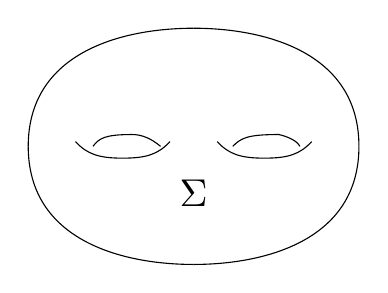
\begin{tikzpicture}[scale=0.6, every node/.style={scale=1.4}]
\draw (-3.5,0) .. controls (-3.5,2) and (-1.5,2.5) .. (0,2.5);  % these 2 lines draw the top half of the donut, made up of 2 arcs
\draw[xscale=-1] (-3.5,0) .. controls (-3.5,2) and (-1.5,2.5) .. (0,2.5);
\draw[rotate=180] (-3.5,0) .. controls (-3.5,2) and (-1.5,2.5) .. (0,2.5); % these 2 lines draw the bottom of the donut, the outside line of the donut, made up of 2 arcs
\draw[yscale=-1] (-3.5,0) .. controls (-3.5,2) and (-1.5,2.5) .. (0,2.5); 


\draw(-2.5,.1) .. controls (-2.25,-0.17) and (-2.0,-0.25) .. (-1.5, -.25) ..  controls (-1., -0.25)  and (-0.75,-0.17) .. (-0.5, .1);
\draw(-2.13,0) .. controls (-2.0,0.17) and (-1.88,0.25) .. (-1.3,.25) .. controls (-1.1,0.25) and (-0.9,0.17) .. (-0.7,0);
\draw( 0.5,.1) .. controls (0.75,-0.17) and (1.0,-0.25) .. (1.5, -.25) ..  controls (2.0, -0.25)  and (2.25,-0.17) .. (2.5, .1);
\draw(0.83,0) .. controls (1.0,0.17) and (1.12,0.25) .. (1.8,.25) .. controls (1.81,0.25) and (2.17,0.17) .. (2.25,0);
\node (S) at ( 0, -1.0) {$\Sigma$};
\end{tikzpicture}  $ \leadsto \mathcal{H}_{\Sigma}$  \quad \quad \quad \, 
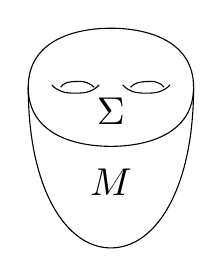
\begin{tikzpicture}[scale=0.3, every node/.style={scale=1.4}]
\draw (-3.5,0) .. controls (-3.5,2) and (-1.5,2.5) .. (0,2.5);  % these 2 lines draw the top half of the donut, made up of 2 arcs
\draw[xscale=-1] (-3.5,0) .. controls (-3.5,2) and (-1.5,2.5) .. (0,2.5);
\draw[rotate=180] (-3.5,0) .. controls (-3.5,2) and (-1.5,2.5) .. (0,2.5); % these 2 lines draw the bottom of the donut, the outside line of the donut, made up of 2 arcs
\draw[yscale=-1] (-3.5,0) .. controls (-3.5,2) and (-1.5,2.5) .. (0,2.5); 

\draw(-2.5,.1) .. controls (-2.25,-0.17) and (-2.0,-0.25) .. (-1.5, -.25) ..  controls (-1., -0.25)  and (-0.75,-0.17) .. (-0.5, .1);
\draw(-2.13,0) .. controls (-2.0,0.17) and (-1.88,0.25) .. (-1.3,.25) .. controls (-1.1,0.25) and (-0.9,0.17) .. (-0.7,0);
\draw( 0.5,.1) .. controls (0.75,-0.17) and (1.0,-0.25) .. (1.5, -.25) ..  controls (2.0, -0.25)  and (2.25,-0.17) .. (2.5, .1);
\draw(0.83,0) .. controls (1.0,0.17) and (1.12,0.25) .. (1.8,.25) .. controls (1.81,0.25) and (2.17,0.17) .. (2.25,0);
\node (S) at ( 0, -1.0) {$\Sigma$};
\node (M) at ( 0, -4.0) {$M$};
\draw (-3.5,0) .. controls (-3.5,-4.3) and (-1.9,-6.8) .. (0,-6.8)
  .. controls (1.9,-6.8)   and (3.5,-4.3)  .. ( 3.5,0);
\end{tikzpicture} $ \leadsto Z(M) \in \mathcal{H}_{ \Sigma}$
\end{center}
\caption{TQFT}
\end{figure}


\section{Chern-Simons theory and the Jones polynomial }\label{Sec:CStheoryJonespoly}

As mentioned, the Wilson loop observable in representation $R$ is a topological invariant that corresponds to a knot $K$ in $M$.  Let the 3-manifold $M$ have a boundary $\Sigma = \partial M$.

For a knot $K$, the path integral, with the Wilson line observable, $W_R{(K)}$, inserted, from \eqref{Eq:Wilsonline00}, yields the following partition function:
\begin{equation}
  Z_{\text{CS}}{ (M; K)} = \int DA \exp{ \left( \frac{ik}{4\pi } S_{\text{CS}}{ (A)} \right)} W_R{(K)}  \label{Eq:ZforWilsonlineCS}
\end{equation}
Witten had shown that Chern-Simons theory in representation $R$ for Lie algebra $\mathfrak{g}$ of gauge group $G$ was exactly solvable \cite{Witten1989}.  Specifically, as \eqref{Eq:ZforWilsonlineCS} is manifestly a topological invariant, $Z_{\text{CS}}{(M;K)}$ can be computed and is exactly equal to a knot invariant, namely, the Jones polynomial,  $J^{\mathfrak{g},R}{ (K;q)}$.  The Jones polynomial is a polynomial in $q$ \cite{Witten1989}. $q$ is the following, in terms of the level $k$ and gauge group $G=SU(2)$:
\[
q = e^{  \frac{ 2\pi i }{ k + 2 }}
\]


To solve the theory exactly, the Hilbert space $\mathcal{H}_{\Sigma}$ and the operators on it, namely the braiding operator, can be constructed from the conformal blocks of a conformal field theory and from the representations of the corresponding modular group.  For Chern-Simons theory, and for this work in particular, the relevant conformal field theory is the $G/G$ WZW model, where $G=SU(N)$.  Note that representations of the modular group needed are simply the $S$ and $T$ matrices, unitary representations of the action of modular group $SL(2,\mathbb{Z})$, such that (as a reminder):
\begin{equation}
S^4=1 \quad \quad \, (ST)^3 = S^2
\end{equation}
on $\mathcal{H}_{\Sigma}$.

With the appropriate $S$, $T$, and braiding matrices, one can solve the theory on any 3-manifold $M$.  This way, the knot invariants in Chern-Simons theory can be explicitly computed.

The space of conformal blocks will play a role in the construction of the Hilbert space $\mathcal{H}_{\Sigma}$.  Consider $\mathbb{C}P^1$ and $n=4$ distinct points living in it, $p_1, \dots , p_4$.  Denote $z_j$ the coordinate $z{(p_j)}$ of the point $p_j$.  For each point, associate a highest weight representation $H_{\lambda_1}, \dots , H_{\lambda_4}$ for highest weight $\lambda_1, \dots \lambda_4$, respectively.  One reexpresses the four point correlation function, say  $\langle \phi_1(z_1, \overline{z}_1) \phi_2{ (z_2,\overline{z}_2) }\phi_3{ (z_3,\overline{z}_3) }\phi_4{ (z_4,\overline{z}_4) } \rangle$, after considering the invariance (under M\"{o}bius transformations) of ratios involving $z_1, \dots ,z_4$ and operator algebra, into a sum of contributions from different representations.  The functions in this sum are the conformal blocks \cite{DiFrancesco1999}.

As a prescient example, consider the four point function $\phi_Q{ (R,R,\overline{R}, \overline{R})}$ such that each of the points carry a representation $R_a = R$ or $\overline{R}$ for $a= 1, \dots 4$, and $Q \in R \otimes R$, with $Q$ being an intermediate conformal family.  The conformal block can be represented by a tree diagram with four legs:

\begin{figure}[h]
\begin{center}
  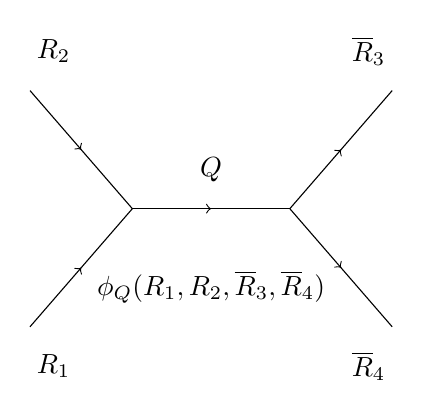
\begin{tikzpicture}
\begin{scope}[decoration={
    markings,
    mark=at position 0.5 with {\arrow{>}}}
    ] 
    \draw[postaction={decorate}] (-2.3,1.5) -- ( -1,0 );
    \draw[postaction={decorate}] (-1,0) -- (1,0);
    \draw[postaction={decorate}] (1,0) -- (2.3,1.5);
    \draw[postaction={decorate}] (-2.3,-1.5) -- (-1,0)  ;
    \draw[postaction={decorate}] (1,0) -- (2.3,-1.5);
\end{scope}
\node at (0,0.5) {$Q$};
\node at (-2,2.0) {$R_2$};
\node at (-2,-2.0) {$R_1$};
\node at (2,2.0) {$\overline{R}_3$};
\node at (2,-2.0) {$\overline{R}_4$};
\node at (0, -1.0) {$\phi_Q{ (R_1, R_2, \overline{R}_3, \overline{R}_4)}$};
\end{tikzpicture}
\end{center}
\caption{Conformal block $\phi_Q{ (R_1, R_2, \overline{R}_3, \overline{R}_4) }$ for the four-point function}
\end{figure}

Finally, the exact relationship between the Jones polynomial and Chern-Simons theory is this: for $G=SU(2)$ in the fundamental representation $R$, for the knot $K$ embedded in a 3-sphere $\mathbf{S}^3$, the following relation was obtained \cite{Witten1989}:
\begin{equation}
J^{\mathfrak{g}, R}{ (K;q) } = \frac{ Z_G^{ \text{CS}}{ (\mathbf{S}^3, K_R;q) } }{ Z^{\text{CS}}_G{ (S^3, \circlearrowleft_R;q) } }  \label{Eq:CStheoryJonespolynomial00}
\end{equation}
where $k$ is the level, $q = \exp{ \left( \frac{2\pi i}{ k + 2} \right) }$, and $\circlearrowleft$ denotes the unknot.  


\chapter{Knot Theory} \label{chap:KnotTheory}

In this chapter, basic notions in the mathematical theory of knots will be presented.  It should be noted that one of the aims is to try to show how the Kauffman bracket and Reidemeister moves play a role in the Jones polynomial knot invariant.  The following knot invariants - Jones polynomial, HOMFLY-PT polynomial, their respective colored versions, and the A-polynomial - are introduced as they will be indispensable in this work.  

\begin{quote}
In other words, personally what I care about are not the knots but the connections between the knots and quantum physics. -\emph{Edward Witten}
\end{quote}

\section{Basic notions}

By a knot, for some smooth embedding $k$ of circle $S^1$ in $\mathbb{R}^3$ (or sphere $S^3$), the image of the embedding is the knot $K$, i.e. 
\[
k : S^1 \hookrightarrow S^3, \quad \, K \equiv \text{im}{k}
\]
A \emph{link}, $L$, is a finite disjoint union of knots, i.e. $L = \coprod_{i=1}^n K_i$ with each knot $K_i$ being a \emph{component} of the link.  

Note that what's interesting about knots is not necessarily the topology of knots, as every knot is homeomorphic to $S^1$, but how the knot $K$ is embedded in the ambient space, either $\mathbb{R}^3$ or $S^3$.  

An \emph{unknot} is a knot $K$ if it bounds an embedded piecewise linear disc in $S^3$.  



%\begin{wrapfigure}{r}{30mm}
\begin{figure}[h]
\begin{center}
\begin{picture}(2,2)
  \put(1,1){\circle{90}}
\end{picture} \quad \quad \quad \quad \quad 
$
\xygraph{
  !{0;/r3.5pc/:}
  !{\vcap-}
  !{\vcap=>}
}
$
%\scalebox{4}{ $\circlearrowleft$ }
\end{center}
\caption{ The Unknot - nonoriented (left) and oriented (right) }
\end{figure}
%\end{wrapfigure}

Recall that a homotopy of a topological space $X \subset \mathbb{R}^3$ is a continuous map $h: X \times [0,1] \to \mathbb{R}^3$. The restriction of $h$ to $t \in [0,1]$ is $h_t:X\times \lbrace t \rbrace \to \mathbb{R}^3$.  But homotopy allows a curve to pass through itself so that all knots are homotopic to the unknot. Try defining an \emph{isotopy} $h$ to be a homotopy such that each $h_t$ is one-to-one.  

Unfortunately, the isotopy doesn't help either. All knots are isotopic to the trivial knot. To see why, imagine pulling on the thread really hard so that the knot becomes very small and tight. Because mathematical threads have no thickness, the mathematical knot and its crossings shrink down into a point and disappears.  

To fix this problem, ensure that the space containing the knot moves continuously along with the knot.  One way to think about this is to imagine the knot embedded in a viscous syrup; stirring the syrup also causes the knot to move.  

Thus, define the notion of two knots, $K_1,K_2$ being \emph{ambient isotopic} to each other: for three-manifold $M = \mathbb{R}^3$ or $S^3$, $K_1, K_2$ are ambient isotopic if there is an isotopy $h: M \times [0,1] \to M$ such that $h(K_1, 0) = h_0(K_1) = K_1$ and $h(K_1,1) = h_1(K_1) = K_2$

And thus two knots are equivalent (or, if you must, belong to the same equivalence class) if they are ambient isotopic.  

One way to get a handle on mathematically understanding a knot is to consider its projection onto a two-dimensional plane.   Consider a plane $h \subset \mathbb{R}^3$ and the projection of the knot onto it. This projection results in a quadrivalent graph (i.e. nodes have degree $4$) embedded in the plane. Each node or vertex is going to be where there is a double point, i.e. when the projection maps two points of the knot onto one point in the plane of the diagram.  The diagram convention is to make breaks in the line corresponding to the strand of the knot that is passing underneath, so that information about the relative height is added at each double point.  The double points in the projection are called a \emph{crossing}.  The \emph{crossing number} of a knot is the minimal number of crossings needed for a knot diagram. 

A link is \emph{oriented} if a direction is assigned to each component of a link.  Such an assignment of a direction to a component will be indicated by one or more arrows drawn on the arcs of the link diagram in the plane.  

Following the direction on an oriented knot diagram, a knot is called \emph{alternating} if at each successive crossing that's traversed, one alternates between going ``over'' and ``under'' until returning to the starting point.

With this ``over'' and ``under'' crossing business for an oriented knot, each crossing in a diagram of an oriented link can be allocated a sign; the crossing is said to be positive or negative, or to have sign $+1$ or $-1$. The convention uses orientations of both strands appearing at the crossing and also the orientation of the ambient space. A positive crossing shows one strand (either one) passing the other in the manner of a ``right-hand screw.''  Note that, for a \emph{knot}, the sign of a crossing does not depend on the knot orientation chosen, for reversing orientations of both strands at a crossing leaves the sign unchanged.  

\begin{figure}[h]
\[
\begin{gathered}
\mathbf{+1 } \quad \, \xygraph{ 
  !{0;/r2.0pc/:}
  !{\xoverv[-1]=>}
  } \quad \quad \quad \, 
\xygraph{
  !{0;/r2.0pc/:}
  !{\xunderv[-1]=>}
  }
\quad \, \mathbf{-1}
\end{gathered}
\]
\caption{positive (negative) crossing convention } \label{Fig:CrossingConvention}
\end{figure}

Indeed (and to set notation), let $\chi$ be the set of crossings of a knot $K$ or link $L$, more generally.  Let $n = |\chi |$.  Number the crossings in some arbitrary way.  Let $n_+$ be the number of right-handed crossings in $\chi$.  Let $n_-$ be the number of left-handed crossings in $\chi$.  





\subsection{Torus Knots } 

A torus knot is a knot that lies on the surface of a torus in $\mathbb{R}^3$.  Each torus knot is specified by coprime integers $m$ and $n$ and isdenoted by $T^{(m,n)}$.  The $(m,n)$-torus knot winds $n$ times around a circle in the interior of the torus, and $m$ times around its axis of rotational symmetry.  There are two distinguished curves on the torus: the \emph{meridian} is $T^{(0,1)}$ and the \emph{longitude} is $T^{(1,0)}$.  Thus, $T^{(m,n)}$ winds $m$ times around the meridian and $n$ times around the longitude. 

The crossing number of a $(m,n)$ torus knot with $m,n >0$ is given by the following:
\[
c = \text{min}{ ((m-1)n, (n-1)m ) }
\]

For the case of $m=2$ (following along the knot, one wraps around the axis of rotation of the whole torus twice), consider for $n=3$ that we obtain 3 crossings.  This torus knot is the \emph{trefoil}.  The trefoil is denoted by $\mathbf{3}_1$, with the subscript $1$ being by tradition, and can also be denoted by $T^{(2,3)}$, as it is part of the family of torus knots.

Note that all torus knots are chiral - a chiral knot is not equivalent to its mirror image.  

\subsection{Twist knot}

A twist knot is a knot obtained by repeatedly twisting a closed loop and then linking the ends together.  A twist knot with $n$ half-twists has crossing number $n+2$.  

\subsection{Reidemeister moves }

Now in 1927, mathematician Kurt Reidemeister proved that all ambient isotopic changes of a knot or link diagram can be obtained by performing, repeatedly if necessary, three basic motions, Reidemeister moves, applied just to small portions of the diagrams in and around crossings, along with simple deformations in the plane, called \emph{plane isotopies}, which do not change any of the crossings of the diagram.  

The Reidemeister moves are of three types, each replacing a simple configuration of arcs and crossings inside of a disc excavated out of the knot diagram by another configuration.  A Type I move inserts or deletes a ``kink'' in the diagram; Type III moves preserves the number of crossings.  Any homeomorphism of the plane must, of course, preserve all crossing information.  


\begin{figure}[h]
\[ 
\begin{gathered}
  \xygraph{
      !{0;/r1.0pc/:}
      [u]
      !{\vover}
      !{\vcap-}
      [ul]!{\xcaph@(0)}
      [r]!{\xcaph@(0)}
     } \, \leftrightarrow \,
     \xygraph{
      !{0;/r1.0pc/:} [uu]
      !{\xcaph[3]@(0)}
   }  \quad \, \text{ \textbf{ Type I }}
\quad \quad \quad \, 
  \xygraph{
      !{0;/r1.0pc/:}
      [u(0.8)]
      !{\xcaph@(0)}
      !{\vover}
      !{\vunder-}
      [l]!{\xcaph@(0)}
      [r]!{\xcaph@(0)}
      [uul]!{\xcaph@(0)}
    } \, \leftrightarrow \,
    \xygraph{
      !{0;/r1.0pc/:}
      [u(0.8)]!{\huncross[2]}
    } 
\quad \, \text{ \textbf{ Type II } } \\
\quad \quad \, \\
  \xygraph{
      !{0;/r1.0pc/:}
      [u(0.7)]
      !{\xoverh[3]}
      [ull][ul(0.5)]!{\sbendv@(0)}
      [rrrr]!{\sbendh@(0)}
      [llllll][d(1.25)]!{\xcaph[-6]@(0)}
    } \, \leftrightarrow \,
    \xygraph{
      !{0;/r1.0pc/:}
      [uu]
      !{\xoverh[3]}
      [lldddd][ld(0.5)]!{\sbendh@(0)}
      [rrrr]!{\sbendv@(0)}
      [llllll][u(1.25)]!{\xcaph[-6]@(0)}
} \quad \, \text{ \textbf{ Type III } }
\end{gathered}  
\]
\caption{ The Three types of Reidemeister moves.  Note that Type III keeps the number of crossings the same. }
\end{figure}

It's obvious that a finite sequence of Reidemeister moves will not change a knot or link presented by a planar projection diagram.  What's more remarkable and useful is the converse.  

\begin{theorem}
  Two link diagrams in the plane represent equivalent links iff one can be converted into the other by a finite sequence of Reidemeister moves and plane isotopies.  
\end{theorem}

\section{Knot Invariants }

\subsection{The Jones Polynomial }\label{subsec:TheJonesPolynomial}

\begin{quote}
 The Jones polynomial, in many ways, is very unusual. It's very modern and near the frontier of contemporary mathematics, and if you want to understand it fully, there's a vast theory; but at the same time, it could be defined in such an elementary fashion that one could teach about it in high school without compromising very much.  -\emph{Edward Witten }
\end{quote}

Consider the following crossing for a knot (link) diagram: 
\[
\xygraph{ 
  !{0;/r1.0pc/:}
  [u(0.5)]
  !{\xoverv}
  }
\]

The  diagrams $\xygraph{
  !{0;/r1.0pc/:}
  [u(0.5)]
  !{\xunoverh} }$ and $\xygraph{
    !{0;/r1.0pc/:}
    [u(0.5)]
    !{\huncross}
    }$ are called the $0$-smoothing and $1$-smoothing of  $\xygraph{ 
  !{0;/r1.0pc/:}
  [u(0.5)]
  !{\xoverv}
  }$, respectively.  




\begin{definition}
  The Kauffman bracket is a function from link diagrams in the oriented plane to Laurent polynomials a formal parameter $q$ with integer coefficients.  So it maps diagram $D$ to $\langle D \rangle \in \mathbb{Z}[q^{1/2}, q^{-1/2}]$ and is characterized by the following properties:
\begin{enumerate}
\item[(i)] $\langle \circlearrowleft \rangle = 1$
\item[(ii)] $\langle D \coprod \circlearrowleft \rangle = ( - q^{1/2} - q^{-1/2}) \langle D \rangle$
\item[(iii)] $\langle \xygraph{ 
  !{0;/r1.0pc/:}
  [u(0.5)]
  !{\xoverv}
  }
  \rangle = q^{-1/4} \langle \xygraph{
    !{0;/r1.0pc/:}
    [u(0.5)]
    !{\huncross}
    }
\rangle + q^{1/4} \langle \xygraph{
  !{0;/r1.0pc/:}
  [u(0.5)]
  !{\xunoverh} }
\rangle$
\end{enumerate} \label{Def:KauffmanBracket}
\end{definition}
Observe that here $D\coprod \circlearrowleft$, for the definition (\ref{Def:KauffmanBracket}) for the Kauffman bracket, signifies that the diagram consists of the diagram $D$ together with an extra unknot that contains no crossings at all, not with itself nor with $D$.  

%It could be proved directly from the definition for the Kauffman bracket, (\ref{Def:KauffmanBracket}), that the following lemmas on how the Kauffman bracket changes (or doesn't change) under Reidemeister moves \cite{Lickorish1997} hold true:  
%\begin{lemma}
%  If a diagram is changed by Type I Reidemeister move, its bracket polynomial changes in the following way:
%\[
% \langle \xygraph{ 
%!{0;/r0.5pc/:}
%      [u]
%      !{\vover}
%      !{\vcap-}
%      [ul]!{\xcaph@(0)}
%      [r]!{\xcaph@(0)}
%  }
%  \rangle = -q^{3/2} \langle 
%\xygraph{
%  !{0;/r0.5pc/:} [uu]
%  !{\xcaph[3]@(0)}
%}
%\rangle , \quad \quad \, 
%\langle
%\xygraph{ 
%  !{0;/r0.5pc/:}
%      [u]
%      !{\vunder}
%      !{\vcap-}
%      [ul]!{\xcaph@(0)}
%      [r]!{\xcaph@(0)}
%  }
%  \rangle 
%= -q^{-3/2} \langle 
%\xygraph{
%  !{0;/r0.5pc/:} [uu]
%  !{\xcaph[3]@(0)}
%}
%\rangle
%\]
%\end{lemma}

%\begin{lemma}
%  If a diagram $D$ is changed by a Type II or Type III Reidemeister move, then $\langle D \rangle$ does not change.
%\end{lemma}

The theory of Jones polynomial rests upon the fact that if the diagram is changed by a Reidemeister move, the polynomial stays the same.  

Formally the Jones polynomial $J(L)$ of oriented link $L$ is a Laurent polynomial in $q^{1/2}$:
\begin{definition}
  The Jones polynomial $J(L)$ of an oriented link $L$ is the Laurent polynomial in $q^{1/2}$, with integer coefficients, defined by 
\begin{equation}
  J(L) =  \left( (-1)^{n_-} (q)^{ (n_+ -2n_-)/2  }  \langle D \rangle \right)_{  } \in \mathbb{Z}[q^{-1/2}, q^{1/2} ]   \label{def:Jonespoly}
\end{equation}
where $D$ is any oriented diagram for $L$
\end{definition}

To compute $J(L)$, $J(L)$ can be computed by using the following skein relation:


\begin{equation}
q J( \xygraph{
  !{0;/r1.3pc/:}
  [u(0.5)]!{\xoverv[-1]=>}
})  -q^{-1 }J(  \xygraph{
  !{0;/r1.3pc/:}
  [u(0.5)]!{\xunderv[-1]=>}
  } ) = (q^{1/2}- q^{-1/2} ) J( \xygraph{
  !{0;/r1.3pc/:}
  [u(0.5)]!{\xunoverv[-1]=>}
} )
\end{equation}

For instance, the Jones polynomial of a (right-handed) torus knot is given by the following:
\[
q^{ (m-1)(n-1)/2 } \frac{ 1 - q^{m+1} - q^{n+1} + q^{m+n} }{ 1-  q^2 }
\]

For $m=2$, this becomes the following:
\[
J(T^{(2,n)} ) = q^{ (n-1)/2 } \frac{ 1 - q^3 - q^{n+1} + q^{2 + n } }{ 1 - q^2 }
\]
For the trefoil, $n=3$, this becomes the following:

\begin{equation}
J(\mathbf{3}_1;q) =  -q^{4} + q^{3} + q
\end{equation}


The Jones polynomial for a figure 8 knot, a twist knot with 4 crossings, denoted by $\mathbf{4}_1$, is the following:
\begin{equation}
J(q;\mathbf{4}_1) = q^{2} - q - \frac{1}{q} + \frac{1}{q^{2}} + 1 
\end{equation}

Notice that there is a symmetry between $q$ and $q^{-1}$, i.e. $J(q^{-1}) = J(q)$: this reflects the fact that the figure-eight knot is achiral, i.e. this oriented knot is equivalent to its mirror image.  

The Jones polynomial was used to prove a number of impressive results.  It resolved Tait's conjecture in that all prime, alternating knots were proven to have an even crossing number.  Also, for a prime, alternating knot with a connected, reduced, alternating diagram of $n$ crossings, the prime knot cannot have a diagram of no less than $n$ crossings; it has a minimum crossing number \cite{Lickorish1997}.  

The Jones polynomial, however, cannot detect chirality for all knots.  If $J(q;K) \neq J(q^{-1};K)$, then the knot $K$ is chiral, but the converse is not true.  

\subsection{Colored Jones polynomial}

Suppose for an oriented knot $K$, we take also the Lie algebra $\mathfrak{g} = \text{sl}{(2)}$ and its  $n$-dimensional irreducible representation $R$, and construct the ``quantum'' $sl{(N)}$ invariant, denoted by $J_n(K;q)$.  %Note that we will sometimes write $J_N(K)$ for the polynomial $P_N$ associated to a knot $K$, suppressing the variable $q$. $J_2{(K;q)   %Think of $q$ right now as a formal variable, or indeterminate.  
$J_2{(K;q)}$ is just the Jones polynomial.  In Chern-Simons theory with gauge group $G=SU(2)$, one could think of $J_n{ (K;q)}$ as the expectation value of the Wilson loop operator on $K$, in the $n$-dimensional representation of $SU(2)$, as mentioned in \eqref{Eq:CStheoryJonespolynomial00} \cite{GukovSaberi2012}.

$J_n(K;q)$ can also be computed directly from a knot diagram using the following skein relation:
\begin{equation}
q^{n/2} J_n( \xygraph{
  !{0;/r1.3pc/:}
  [u(0.5)]!{\xoverv[-1]=>}
})  -q^{-n/2 }J_n(  \xygraph{
  !{0;/r1.3pc/:}
  [u(0.5)]!{\xunderv[-1]=>}
  } ) = (q^{1/2}- q^{-1/2} ) J_n( \xygraph{
  !{0;/r1.3pc/:}
  [u(0.5)]!{\xunoverv[-1]=>}
} )  \label{Eq:coloredJonespolynomialskeinrelation}
\end{equation}


To apply the skein relation \eqref{Eq:coloredJonespolynomialskeinrelation}, one needs to fix the normalization by specifying $J_n{(\circlearrowleft)}$, the colored Jones polynomial of the unknot.  Consider the following choice:

\begin{equation}
  J_n{( \circlearrowleft )} = \frac{ q^{n/2} - q^{-n/2}}{ q^{1/2} - q^{-1/2} } = \underbrace{ q^{ -(n-1)/2 } + q^{ - (n-3)/2 } + \dots + q^{ (n-1)/2 } }_{ n \text{ terms } }  \label{Eq:coloredJonespolynomialunknot00}
\end{equation}
Note that with the choice of normalization for the unknot in \eqref{Eq:coloredJonespolynomialunknot00}, in the so-called classical limit of $q\to 1$, we have the following:
\begin{equation}
  J_n{ (\circlearrowleft)} \xrightarrow{ q\to 1} n
\end{equation}
Again, for the fundamental representation $R$ of $sl{(N)}$, $n$ is the dimension of the representation.  This leads to a generalization of the notion of dimension, called the \emph{quantum dimension} $\text{dim}_q{ (R)}$ of the representation $R$, arising from the quantum group invariant constructed with representation $R$, evaluated on the unknot.  

Note that for $n=2$, the quantum dimension is the following:
\begin{equation}
\text{dim}_q{ R} = q^{1/2} + q^{-1/2} \label{eq:unknotqdim}
\end{equation}

Another choice of normalization is the following:
\begin{equation}
  J_n{ (\circlearrowleft)} = 1 \label{Eq:refinedunknot00}
\end{equation}
One should also note that for theories with the normalization as given in \eqref{Eq:coloredJonespolynomialunknot00}, the theory is called ``unrefined'' and for theories with the normalization given in \eqref{Eq:refinedunknot00}, the theory is ``refined.''  


%Also, the colored Jones polynomial obeys the following relations, known as \emph{cabling formulas}, which follow directly from the rules for the Chern-Simons TQFT \cite{GukovSaberi2012}:

%\begin{equation}
%  \begin{aligned}
%    J_{ \oplus_i R_i }{ (K;q) } & = \sum_i J_{R_i}{ (K ;q)} \\ 
%    J_R{ (K^n;q)} & = J_{R^{ \otimes n } }{ (K;q) }
%\end{aligned}
%\end{equation}
%where $K^n$ is the $n$-cabling of the knot $K$, obtained by taking the path $K$ and tracing it with a ``cable'' of $n$ strands.  The first rule says that if $R$ is reducible, then $J_R$ splits as a sum over irreducible components.  The second rule says that the $R$-colored Jones polynomial for the $n$-cabling of a knot is equal to the colored Jones polynomial of the original knot, but in representation $R^{\otimes n}$.  



\subsection{HOMFLY-PT polynomial}

A generalization of the Jones polynomial is the knot polynomial in two (formal or indeterminate) variables, $a$ and $q$, called the HOMFLY-PT polynomial, $P_{a,q}(L)$, for a link $L$.  The proof of its unique existence has been done, and while the proof is harder than the one for the Jones polynomial, the proof simply relies on induction on the number of crossings, so that the skein relation holds at each step.  To show that the HOMFLY-PT is a knot (link) invariant, once again, for a diagram $D$ for link $L$, the HOMFLY-PT polynomial $P_{a,q}(D)$ is shown to be unchanged by Reidemeister moves on $D$ \cite{Lickorish1997}.   

\begin{theorem}
  There exists a unique function 
\[
  P_{a,q}: \lbrace \text{Oriented links in $S^3$} \rbrace \to \mathbb{Z}[a^{\pm 1 }, q^{ \pm 1/2 } ]
\]
such that $P_{a,q}$ takes the value of $1$ on the unknot and $P_{a,q}$ obeys the following skein relation:

\begin{equation}
a P_{a,q}( \xygraph{
  !{0;/r1.3pc/:}
  [u(0.5)]!{\xoverv[-1]=>}
})  -a^{-1 }P_{a,q}(  \xygraph{
  !{0;/r1.3pc/:}
  [u(0.5)]!{\xunderv[-1]=>}
  } ) = (q^{1/2}- q^{-1/2} ) P_{a,q}( \xygraph{
  !{0;/r1.3pc/:}
  [u(0.5)]!{\xunoverv[-1]=>}
} )
\end{equation}
where $P_{a,q}(L)$ is called the HOMFLY-PT polynomial of the oriented link $L$.  
\end{theorem}

As a knot invariant, the HOMFLY-PT cannot distinguish between simple pairs of knots and links called \emph{mutants}.  The operation of \emph{mutation} involves drawing a disc on a knot diagram such that there are two incoming and two outgoing strands passing through the disc's boundary, and then rotating the portion of the knot inside the disc and reconnecting the strands in a different manner.  The following theorem was proven \cite{Lickorish1997}:

\begin{theorem}
  The HOMFLY-PT polynomial, $P(L)$, is unchanged by mutation of $L$.  
\end{theorem}
The HOMFLY-PT polynomial cannot distinguish between mutants.  Indeed, consider knots $8_8$ and $10_{129}$.  It can be calculated that they both have the same HOMFLY-PT polynomial.  But yet their minimal crossing numbers, $8$ and $10$, distinguishes the knots to be different.  

\subsection{Colored HOMFLY-PT polynomial}

Just as there was a colored Jones polynomial, there is a colored version of the HOMFLY-PT polynomial, the colored HOMFLY-PT polynomial, $P_{\lambda}{(L;a,q)}$ that in general has associated to it the Young diagram $\lambda$, i.e. 2-dimensional partitions, for the representation of $sl{(N)}$.  However, in this work, the only Young diagrams that will be considered are Young diagrams consisting only of a single row (or a single column).  By the Schur-Weyl duality, Young diagrams consisting of a single row (or a single column) correspond to totally symmetric (or totally anti-symmetric) representations.  They are $n$-dimensional fundamental representations of the Lie algebra $\mathfrak{g}$.  

$P_0{(L)}$ yields the Alexander polynomials of $L$.  $P_2{(L)}$ yields the Jones polynomials of $L$.  $P_1{(L)}$ is the trivial invariant.  
%For $n>0$, the polynomial $P_n{(L)}$ can be interpreted via representation theory of quantum $sl{ (N)}$ \cite{Khovanov2006}.

\section{A-polynomial}  \label{Sec:Apolynomial}

The two-variable $A$-polynomial, a knot invariant, defined using representations of the fundamental group of the knot complement into $SL{(2,\mathbb{C})}$ was introduced by Cooper, Cullen, Gillert, Long and Shalen \cite{CooperCullerGillertLongShalen1994}.  A review with a slightly different approach was made later \cite{CooperLong1996}.  

Consider a knot $K$ embedded into 3-sphere $\mathbf{S}^3$.  Let $N(K)$ be the open tubular neighborhood of the knot $K$.  $N$ is homeomorphic to a solid torus, i.e. $N \cong \mathbf{D}^2 \times \mathbf{S}^1$.  The knot complement is defined as the following:
\begin{equation}
  M = \mathbf{S}^3 \backslash N(K)
\end{equation}
and the knot complement $M$ is a compact 3-manifold whose boundary $\partial M$ is a torus, $\Sigma = T^2$.  

The knot group is the fundamental group of the knot complement: $\pi_1(M)$.  Consider representations of the knot group into the complex gauge group $SL{(2,\mathbb{C})}$, i.e. consider homomorphisms $\rho$ s.t.
\[
\rho: \pi_1(M) \to SL{(2,\mathbb{C})}
\]
Now there is a natural restriction from $M$ to its boundary $\partial M = T^2$ and so one could consider representations on the boundary of $M$ instead:
\[
\rho:\pi_1(\partial M) \to SL{(2,\mathbb{C})}
\]







%Thurston showed that $\rho_0$ can be deformed to give a one complex parameter family of nonabelian representations of $\pi_1{(M)}$ into $SL{ (2,\mathbb{C})}$, modulo a conjugacy, for the hyperbolic knots \cite{Thurston1977}.  However, even non-hyperbolic knots may have such families of representations, as the torus knots do \cite{CooperLong1996}.  



\begin{figure}[h]
\begin{center}
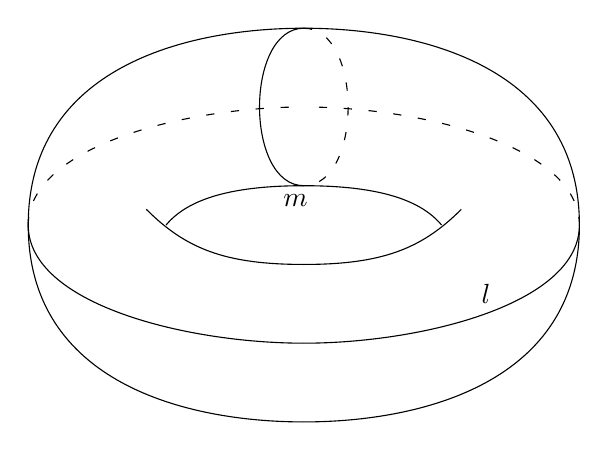
\begin{tikzpicture}
\draw (-3.5,0) .. controls (-3.5,2) and (-1.5,2.5) .. (0,2.5);
\draw[xscale=-1] (-3.5,0) .. controls (-3.5,2) and (-1.5,2.5) .. (0,2.5);
\draw[rotate=180] (-3.5,0) .. controls (-3.5,2) and (-1.5,2.5) .. (0,2.5);
\draw[yscale=-1] (-3.5,0) .. controls (-3.5,2) and (-1.5,2.5) .. (0,2.5);

\draw[loosely dashed] (-3.5,0) .. controls (-3.5,1) and (-1.5,1.5) .. (0,1.5);
\draw[xscale=-1, loosely dashed] (-3.5,0) .. controls (-3.5,1) and (-1.5,1.5) .. (0,1.5);
\draw[rotate=180] (-3.5,0) .. controls (-3.5,1) and (-1.5,1.5) .. (0,1.5) node[pos=.5,above] {$l$} ;
\draw[yscale=-1] (-3.5,0) .. controls (-3.5,1) and (-1.5,1.5) .. (0,1.5);

\draw (0,2.5) .. controls (-0.75, 2.5) and (-0.75, 0.5) .. ( 0, 0.5) node[pos=0.95,below] {$m$} ;
\draw[xscale=-1,loosely dashed] (0,2.5) .. controls (-0.75, 2.5) and (-0.75, 0.5) .. ( 0, 0.5);

\draw (-2,.2) .. controls (-1.5,-0.3) and (-1,-0.5) .. (0,-.5) .. controls (1,-0.5) and (1.5,-0.3) .. (2,0.2);

\draw (-1.75,0) .. controls (-1.5,0.3) and (-1,0.5) .. (0,.5) .. controls (1,0.5) and (1.5,0.3) .. (1.75,0);

\end{tikzpicture}
\caption{The torus $T^2 = \partial N{ (K) }$ for $K = $ unknot, with cycles $m$ and $l$} \label{Fig:toruscycles}
\end{center}
\end{figure}

With $\partial M = T^2$, then $\pi_1{ (\partial M) } = \pi_1{ (T^2)} = \mathbb{Z} \times \mathbb{Z}$.  Let $m$ and $l$ be a basis for $\pi_1{ (T^1)}$, i.e. two generators of the fundamental group that are two basic cycles.  $m$ and $l$ denote the meridian and longitude, respectively, as depicted in Figure \ref{Fig:toruscycles}.  $m$ is the cycle that is contractible when in $N(K)$ and $l$ is the non-contractible cycle.  $l$ follows the knot as the knot is traversed.  

These cycles, $m$ and $l$, are represented in $SL(2,\mathbb{C})$ by $2\times 2$ complex matrices $\rho(m)$ and $\rho(l)$ with determinant $1$.  Since the fundamental group of the torus is just $\mathbb{Z}\times \mathbb{Z}$, the generators or cycles for $T^2$ are abelian, and so the matrices $\rho(m)$, $\rho(l)$ commute.  Since they commute, they can be simultaneously brought to Jordan normal form, an upper triangular form, by some change of basis, i.e. by conjugacy by an element of $SL(2,\mathbb{C})$
\begin{equation}
  \rho(m) = \left( \begin{matrix} x & * \\ 0  & x^{-1} \end{matrix} \right), \quad \, \rho(l) = \left( \begin{matrix} y & * \\ 
    0 & y^{-1} \end{matrix} \right)
\end{equation}

Thus, there is a map such that to each representation of the knot group, the map assigns two complex numbers
\begin{equation}
  \begin{aligned}
    \text{Hom}{ (\pi_1(M), SL(2,\mathbb{C}) )} / \text{ conj. } & \to \mathbb{C}^* \times \mathbb{C}^* \\ 
    \rho & \mapsto (x,y) 
\end{aligned} \label{eq:rep2algcurve}
\end{equation}
where $x$, $y$ are eigenvalues of $\rho(m)$ and $\rho(l)$, respectively. The image of this map is the \emph{representation variety} $\mathcal{C} \subset \mathbb{C}^* \times \mathbb{C}^*$, (note that $\mathbb{C}^* \equiv \mathbb{C} - \lbrace 0 \rbrace$).  

Thurston had showed that for a space $M$ with a single torus boundary, the dimension of $\text{Hom}{ (\pi_1(M), SL{(2,\mathbb{C})} )}$ in \eqref{eq:rep2algcurve} is equal to 4 \cite{Thurston1977}.  On the other hand, the Lie group $SL(2,\mathbb{C})$ has complex dimension 3 and the $SL(2,\mathbb{C})$ matrices are involved in conjugation in \eqref{eq:rep2algcurve}.  Thus, after identifying conjugate representations, we obtain a representation curve, or representation variety, of complex dimension of one.  Furthermore, a basis $(l,m)$ for the boundary of $M$ determines an embedding of $\mathcal{C}$ into $\mathbb{C}^* \times \mathbb{C}^*$, as we've seen, and using the standard techniques from algebraic geometry one can show that the representation variety $\mathcal{C}$ is the zero locus of a single polynomial $A(x,y)$ in two variables.  

Thus, there exists a polynomial, unique up to constant multiples, that defines this representation variety $\mathcal{C}$, an algebraic curve.  This polynomial is the \emph{A-polynomial}.  

%, whose defining polynomial is the $A$-polynomial of $K$.  

Again, note that this definition of the $A$-polynomial does not fix the overall numerical coefficient, which is usually chosen in such a way that $A(x,y)$ has integer coefficients.  

Note that every knot group abelianizes to $\mathbb{Z}$ as the torus $T^2$ is path connected.  So whenever $M$ is a knot complement in $\mathbf{S}^3$, one can have the abelianization of the knot group $\pi_1(M)$, such that its first homology group is abelian: 
\begin{equation}
  \pi_1{ (M)}^{\text{ab}} = H_1{ (M)} \cong \mathbb{Z}
\end{equation}
Thus, every representation of $\mathbb{Z}$ into $SL{(2,\mathbb{C})}$ induces a representation of the knot group.  These \emph{abelian representations} of the knot form a component of the representation variety isomorphic to $SL{(2,\mathbb{C})}$ \cite{CooperLong1996}.  It then turns out that the A-polynomial thus always contains a factor of $y-1$.  $y-1$ is the abelian factor because the longitude $l$, which $y$ is associated to, which was non-contractible in the torus $T^2$, is contractible in $M$, so that $\rho{(l)}$ must be the identity.  

To illustrate the abelian factor of $(y-1)$, consider these examples of the A-polynomial for the torus knot $T^{(2,2p+1)}$ for $p=1$,
\begin{equation}
A{ (T^{2,3}; x,y)} = {\left(x^{3} + y\right)} {\left(y - 1\right)}
\end{equation}
for $p=2$,
\begin{equation}
 A{ (T^{2,5}; x,y)} = {\left(x^{5} + y\right)}^{2} {\left(y - 1\right)}
\end{equation}
and for $p=3$,
\begin{equation}
 A{ (T^{2,7}; x,y)} =  {\left(x^{7} + y\right)}^{3} {\left(y - 1\right)}
\end{equation}
where the A-polynomial factorizes and includes a factor of $(y-1)$ in each case.

Another property that can be checked immediately from the examples above and that holds true in general is that the A-polynomial is reciprocal, i.e. up to an overall factor of powers of $x$ and $y$ in front, 
\begin{equation}
  A(x,y) \sim A(x^{-1},y^{-1}) \label{eq:Apolyreci}
\end{equation}
From this reciprocal property, in the algebraic curve $\mathcal{C}$ defined by the zero locus of the A-polynomial, the points in $\mathcal{C}$ actually lie in $\mathbb{C}^* \times \mathbb{C}^* /\mathbb{Z}_2$.  

One other property is that the A-polynomial can distinguish mirror knots.  The A-polynomial is not invariant under a change of orientation of the ambient space, which is $\mathbf{S}^3$ in this case.  Thus the A-polynomial does a better job than the Jones polynomial as a knot invariant.  How the A-polynomial can distinguish mirror knots can be made explicit with the following:
\begin{equation}
A(x,y) \neq A(x,y^{-1})
\end{equation}
and from \eqref{eq:Apolyreci}, the reciprocal property of the A-polynomial, this could also be stated as $A(x,y) \neq A(x^{-1},y)$.  

Finally, a few remarks could be made for the rational of studying the representations of the knot group into $SL{(2,\mathbb{C})}$.  From Thurston, a knot complement $M$ has a hyperbolic structure if and only if it is not a satellite or a torus knot \cite{Thurston1977}.  With this hyperbolic structure, one would then consider representations of $\pi_1{(M)}$ into the isometries of the hyperbolic space.  Fortunately, this representation lifts to a representation into $SL{(2,\mathbb{C})}$ \cite{CooperLong1996}.

A hyperbolic structure determines an action of $\pi_1{( M)}$ by isometries on the hyperbolic 3-space $\mathbb{H}^3$, determined up to a conjugacy.  As a reminder, $\mathbb{H}^3$ can be defined as the upper half-space with the following standard hyperbolic metric:




To summarize, there is a planar algebraic curve $\mathcal{C}$ that is defined by the zero locus of the $A$-polynomial, i.e. $A(x,y) =0$:
\begin{equation}
\mathcal{C} = \lbrace (x,y) \in \mathbb{C}^* \times \mathbb{C}^*/\mathbb{Z}_2 | A(x,y) = 0 \rbrace \label{eq:algcurveApoly}
\end{equation}
and the A-polynomial is a two variable polynomial invariant of knots defined using representations of the fundamental group of the knot complement into $SL{(2,\mathbb{C})}$








\chapter{$q$-Pochhammer symbols} \label{chap:qPochhammersymbol}

In this brief chapter, the $q$-Pochhammer symbol will be introduced, as it will be used in computations later in this work.  The notion of a $q$-hypergeometric sequence will be introduced and this concept will be needed in Appendix \ref{app:qZeilqMultiSum}.

A hypergeometric sequence $\lbrace c_k \rbrace$, indexed by an integer $k$,  is defined such that the ratio of successive terms in the sequence is a rational function of $k$:
\[
\frac{c_{k+1}}{ c_k } = \frac{P(k)}{ Q(k)}
\]
with $P(k)$ and $Q(k)$ being polynomials in $k$. 

For instance, consider the factorial $f(k) \equiv k!$.  Indeed, this is a hypergeometric sequence since
\[
\frac{ f(k+1)}{ f(k)} = \frac{ (k+1)! }{ k!} = k+1
\]
Recall that $k!$ is the total number of permutations $\sigma$ of $k$ objects.  For a permutation $\sigma$, and an original ordering of $k$ objects, $(1,2, \dots , k)$, then for $i \in 1, 2, \dots , k$, $\sigma(i)$ tells us the new position, after permutation, of the object $i$.  Then for a permutation $\sigma$, an inversion is such that for a pair of the original positions of the objects, $i$ and $j$, with $1\leq i < j \leq k$, then $\sigma(i) > \sigma(j)$.  

Let $\text{inv}{(\sigma)}$ be the total number of inversions of a permutation $\sigma$.  Note that clearly, for a permutation $\sigma$ of $k$ inversions, to put the permutation back into the original ordering, $k$ transpositions (exchanging a pair of objects, while leaving the other objects unchanged) are needed.

Introduce a formal parameter $q$.  For a permutation $\sigma$ with $\text{inv}{(\sigma)}$ total number of inversions, one could imagine doing successive transpositions, up to $\text{inv}{(\sigma)}$ transpositions, to put $\sigma$ back into the original ordering.  Represent this procedure by the factor $(1 + q + q^2 + \dots + q^{ \text{inv}{(\sigma )} -1})$.  

With these ingredients, define the $q$-factorial:
\begin{equation}
[k]_q! \equiv 1 (1 +q)( 1 + q +q^2) \dots (1 + q + \dots + q^{k-1} )  \label{eq:qfactorial}
\end{equation}
The $q$-factorial $[k]_q!$ can also be rewritten in the following form:
\begin{equation}
[k]_q! =   \frac{ ( 1-q)(1-q^2) \dots (1-q^k ) }{ (1-q)^k}
\end{equation}
For the $q$-factorial $[k]_q!$, it is remarkable that the coefficient of $q^i$ in $[k]_q!$ gives the number of permutations of $k$ with $i$ inversions.  Also note that from the definition \eqref{eq:qfactorial}, when $q=1$, the usual factorial is recovered.  

A $q$-hypergeometric sequence $\lbrace f_k \rbrace$, indexed by integer $k$, is defined such that the ratio of successive terms is a rational function of $q^k$:
\[
\frac{f_{k+1}}{ f_k} = \frac{ P{ (q^k)} }{ Q{(q^k)}}
\]
for all the integers $k$ where this ratio is well-defined, and with $P(q^k)$ and $Q(q^k)$ being polynomials in $q^k$.  

For example, the $q$-factorial is $q$-hypergeometric as 
\[
\frac{ [k+1]_q! }{ [k]_q!} = \frac{1-q^{k+1}}{  (1-q)^{k+1}}
\]

Define the $q$-Pochhammer symbol as follows:
\begin{definition}
  The $q$-Pochhammer symbol, $(x,q)_k$, is defined as such:
  \begin{equation}
    (x,q)_k \equiv \prod_{i=0}^{k-1} (1-xq^i) = (1-x)(1-xq) \dots ( 1-xq^{k-1}) = \prod_{i=1}^{k} (1-xq^{i-1})   \label{Def:qPochhammer}
  \end{equation}
\end{definition}
Thus, the $q$-factorial $[k]_q!$ can also be rewritten in the following form:
\[
[k]_q! = \frac{ (q,q)_k}{ ( 1-  q)^k}
\]
The $q$-Pochhammer symbol is also $q$-hypergeometric:
\[
\frac{(x,q)_{k+1}}{ (x,q)_k} = 1 - xq^k
\]

Define the $q$-binomial coefficient as follows:
\begin{definition}
  The $q$-binomial ${ n \brack k }_q$ is defined as such:
\begin{equation}
  { n \brack k }_q = \frac{ (1- q^n) ( 1 - q^{n-1} ) \dots ( 1 - q^{ n- k + 1 }  ) }{ (1- q) ( 1 - q^2 ) \dots ( 1- q^k ) }  \label{Def:qbinomial}
\end{equation} 
\end{definition}

It will be useful to write out explicitly the following identities for the $q$-Pochhammer symbol, from its definition \ref{Def:qPochhammer}:
\begin{equation}
\begin{aligned}
  & (q^{n-1}, q^{-1})_k = \prod_{i=0}^{k-1} ( 1 - q^{n-1} q^{-i} ) = (1-q^{n-1} )(1 - q^{n-2}) \dots ( 1 - q^{n-k} ) \\ 
%  & (q,q)_k = \prod_{i=0}^{k-1} (1 - q \cdot q^i ) = (1-q)(1-q^2 ) \dots (1-q^k) \\
  & \left( \frac{-at}{q}, q \right)_k = \prod_{i=1}^k ( 1 + aq^{i-2}t )
\end{aligned}  \label{Eq:qPochhammerbasic00}
\end{equation}

Clearly, from the above explicit expressions, immediately one obtains the following identity for the $q$-binomial (given in the definition \ref{Def:qbinomial}):
\begin{equation}
  { n \brack k }_q = \frac{ (q^n, q^{-1})_k }{ (q,q)_k}  = \frac{ ( 1 - q^n ) }{ ( 1 - q^{n-k} ) } \cdot  \frac{  (q^{n-1}, q^{-1})_k }{ (q,q)_k } 
\end{equation}
Also, note that the $q$-binomial is also $q$-hypergeometric, being a ratio of $q$-Pochhammer symbols.  


The $q$-Pochhammer symbol $(x,q)_k$ has the following asymptotic behavior when $k$ is large:
\begin{equation}
  (x,q)_k \equiv \prod_{i=0}^{k-1}{ (1-xq^i )} \sim e^{ \frac{1}{ \hbar}{ ( \text{Li}_2{ (x)} - \text{Li}_2{ (xq^k)} ) } } \label{Eq:qPochhammerasymptotics}
\end{equation}
where $\text{Li}_2{(z)}$ is the dilogarithm.  The dilogarithm $\text{Li}_2(z)$ can be expressed as an infinite series for $|z| <1$, with $z$ being a complex number:
\begin{equation}
  \text{Li}_2{ (z) } = \sum_{k=1}^{\infty} \frac{z^k}{k^2 }
\end{equation}


\chapter{Categorification} \label{chap:Categorification}

In this chapter, Khovanov homology will be reviewed.  \cite{Bar-Natan2002} provides a succinct review of Khovanov homology, along with algorithms for computation.  Matrix factorization in Khovanov-Rozansky homology, a homology for $sl{(N)}$ knot homology, will be briefly explained.  The colored superpolynomial will be introduced.  The differentials in the knot homology associated with the colored superpolynomial will be explained, and this chapter includes a number of basic examples of these differentials.  Finally, the expressions for the colored superpolynomials for the family of torus knots and twist knots will be presented.  


\section{Khovanov homology}


In \cite{Khovanov2000}, Khovanov introduced a new invariant for oriented knots and links.  Khovanov's idea was to associate to the plane diagram of a knot or a link a chain complex of vector spaces.  The homology of the chain complexes turns out to be a knot invariant under Reidermeister moves; specifically the alternating sum of the ranks of the homology groups is an Euler characteristic that reproduces the Jones polynomial.  But with the new, extra grading from the knot homology groups, the resulting two-parameter Poincar\'{e} polynomial is an even stronger invariant than the Jones polynomial.  
% that arises as the homology of a chain complex.  The homological knot invariant has the Jones polynomial as its graded Euler characteristic.  

Now, there is no a priori reason why the knot polynomial invariants, in particular, the Jones polynomial, the colored Jones polynomial, or even the colored HOMFLY-PT polynomial, should ``lift'' to a knot homology.  This ``lift'' is called \emph{categorification}.  The term was coined by L. Crane and I. Frenkel \cite{CraneFrenkel1994} in the context of lifting an $n$-dimensional TQFT to a $(n+1)$-dimensional TQFT.  

Indeed, recall axiomatic 3-dimensional TQFT.  One could think of a 3-dimensional TQFT  as a functor $Z$ makes the following assignments:
\[
\begin{aligned}
\text{ closed 3-manifold $M$ }  & \leadsto \text{ number $Z(M)$}  \\
\text{ knot $K \subset M$ }  & \leadsto \text{ polynomial invariant $P(K)$}  \\
\text{ closed 2-manifold $\Sigma$ } & \leadsto \text{ vector space $Z{(\Sigma)} \equiv \mathcal{H}_{\Sigma}$ } 
\end{aligned}
\]

Then the categorification of a 3-dimensional TQFT should be a 4-dimensional TQFT, such that
\[
\begin{aligned}
  Z(M)  \\
  \mathcal{H}_{\Sigma}
\end{aligned} \xrightarrow{ \text{ categorification } } \begin{aligned}
\text{ vector space $\mathcal{H}_K$ } \\
\text{ category $\textbf{Cat}_{\Sigma}$ } \end{aligned}
\]
\cite{CraneFrenkel1994}.  But what about the categorification of the knot polynomial invariant, $P(K)$?  

%\begin{tikzpicture}[scale=0.6, every node/.style={scale=0.6}]
%  \draw (0,0) .. controls (1,2) and (2,-1) .. (1,-2);
%  \draw (2,0) .. controls (3,0) and (3,-1) .. (0,0);
%  \draw (1,-2) ..  controls (-1,-2) and (-1,-1) .. (2,0);
%\end{tikzpicture}

Khovanov's idea was to replace the polynomials for a knot polynomial invariant with graded vector spaces, and turn the Jones polynomial into a homological object.  

\subsection{Spaces }

It would be instructive to follow the pedagogical review in \cite{Bar-Natan2002} to get a grasp of Khovanov homology and the following subsections provide even further elementary explanations. 

\begin{definition}
Let $V = \oplus_{m} V_m$ be a graded vector space. The graded dimension of $V$ is the power series $\text{ dim}_q{V}  \equiv \sum_m q^m \text{dim}{V_m}$  \end{definition}

While the following ``height'' operation will not be used here, introducing the notion height will help to understand the bi-grading (the two gradings) in Khovanov homology.  We will also anticipate a bi-graded homology theory with the notation $\mathcal{C}_{**}$ for the chain complex.

%\begin{definition}
%Let $\lbrace l \rbrace$ be the ``degree shift'' operation on graded vector space i.e. if $V  = \oplus_m V_m$ is a graded vector space, then
%\[
%V \lbrace k \rbrace_m \equiv V_{m-k}
%\]
%so that $\text{ dim}_q{ V\lbrace k \rbrace} =q^k  \text{ dim}_q{V}$
%\end{definition}

\begin{definition} Let $[s]$ be the ``height shift'' operation on chain complexes i.e. if $\mathcal{C} $ is a chain complex 
\begin{center}
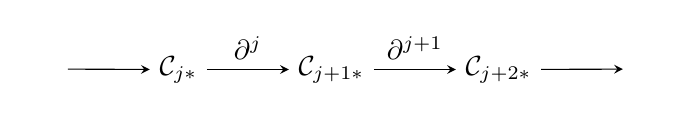
\begin{tikzpicture}
  \matrix (m) [matrix of math nodes, row sep=2em, column sep=3em, minimum width=1em]
  {
 \phantom{c}   & \mathcal{C}_{j*} & \mathcal{C}_{j+1*} & \mathcal{C}_{j+2*} & \phantom{c}   \\   };
  \path[-stealth]
  (m-1-1) edge node  {$$} (m-1-2)
  (m-1-2) edge node [above] {$\partial^j$} (m-1-3)
  (m-1-3) edge node [above] {$\partial^{j+1}$} (m-1-4)
  (m-1-4) edge node [above] {$$} (m-1-5);
\end{tikzpicture}
\end{center}
%$\dots \to  \mathcal{C}^r \xrightarrow{ d^r}  \mathcal{C}^{r+1} \dots $ 
of (possibly graded) vector space (a piece $\mathcal{C}_{j*}$ of that complex has ``height'' $j$) and so the application of the height shift $[s]$ to chain complex, $\mathcal{C}[s]$, then shifts the ``height'' of each of the vector spaces, so that $\mathcal{C}_{j*} \to \mathcal{C}_{j-s*}$, i.e.
%if $\mathcal{C} = \mathcal{C}[k]$, then $\mathcal{C}^r = \mathcal{C}^{r-s}$, i.e.
\begin{equation}
  \mathcal{C}[s]_{j*} \equiv \mathcal{C}_{j-s}
\end{equation}
with $\mathcal{C}_{**}{ [s]}$ denoting the complex $\mathcal{C}_{**}$, shifted $s$ places to the right.  
\end{definition}

Now recall, from the subsection of this work, \ref{subsec:TheJonesPolynomial}, that $\chi$ is the set of all crossings for a link diagram $L$.  For each $\chi$, there are two possible smoothings, $0$-smoothing or $1$-smoothing.  The total number of crossings will be denoted $|\chi|=n$ here.  Thus, a $n$-dimensional cube $\lbrace 0, 1 \rbrace^{\chi}$ is the space of all possible choice of smoothings, at each crossing, for a link diagram.  Each vertex $\alpha \in \lbrace 0 ,1 \rbrace^{\chi}$ of this $n$-dimensional cube is a choice of smoothing for each crossing of a link diagram.  



\subsection{Step 1}

Let $V$ be the graded vector space with two basis elements $v_{\pm}$ whose degrees are $\pm 1/2$, respectively.  Thus for $V$, $\text{dim}_q{V} = \sum_m q^m \text{dim}{ V_m} = q^{1/2} + q^{-1/2}$.  

For each vertex $\alpha \in \lbrace 0 , 1 \rbrace^{\chi}$ of the $n$-dimensional cube $\lbrace 0 , 1 \rbrace^{\chi}$, for link diagram $L$, associate the graded vector space $V_{\alpha}(L) \equiv V^{ \otimes l}{ \lbrace j \rbrace}$, where $l$ is the number of cycles in the smoothing of $L$, $j$ is the height (or, in other words, the number of ``$1$'' smoothings, or, if this helps, which vertex we're on, on the cube), and $|\alpha | =\sum_i \alpha_i$ of $\alpha$.   $\text{dim}_q{ V_{\alpha}{ (L)} }$ is the Laurent polynomial that appears at vertex $\alpha$ in the cube.  

Anticipating the construction of a bigraded chain complex, let the $j$th chain group $\mathcal{C}_{j*}$ be defined as follows: 
\begin{equation}
\mathcal{C}_{j*} \equiv \bigoplus_{ \alpha : j = | \alpha | } V_{\alpha}{ (L)}
\end{equation}

Consider the example of the trefoil.  There are $n = | \chi | = 3$ crossings.  Label each of the crossings with $1$, $2$, or $3$.  All crossings are right-handed: $n_+=3$ and $n_- =0$.  There is a 3-dimensional cube with 8 vertices: $000, 100, 010, 001 , 110, 101, 011, 111$, with each $0$, or $1$ being the choice of $0$-smoothing or $1$-smoothing, respectively, at each crossing, crossing $1, 2,$ or $3$.

For the trefoil, by considering a complete smoothing of the knot, the result can either by only one, two, or three cycles (unknots).  So for the graded space $V_{\alpha}{(L)}$, $l$ can be $1, 2$ or $3$.  Also, the total number of $1$-smoothings sum to the height of the graded vector space, $j$.  There can be $0,1,2$, or $3$ total $1$-smoothings and so $j=0, \dots , 3$.  

After conducting a direct sum of all the vector spaces of equal height $j$, $V_{\alpha}{(L)}$'s, the $j$th chain group $\mathcal{C}_{j*}$ is obtained.  

For each $\mathcal{C}_{j*}$, a Laurent polynomial can be calculated, according to $q^{j/2} \text{dim}_q{ \mathcal{C}_{j*} }$.  Again, note that $\text{dim}_q{V_{\alpha}{(L)}}$ is the Laurent polynomial that appears at vertex $\alpha$.  Anticipating the calculation of the Euler characteristic, include a factor of $(-1)^k$, alternating across the chain group.

So for the trefoil, one could collect the information above on the chain groups $\mathcal{C}_{j*}$:
\begin{equation}
\begin{gathered}
  \begin{matrix}
\text{ Laurent polynomial, } (-1)^k q^{j/2} \text{dim}_q{ \mathcal{H}_{jk}}  &      & \text{ vertices } &  & \text{ height } j  & \text{ cycles } l \\ 
   (q^{1/2} + q^{-1/2})^2   &  & 000 &  &  0    & 2 \\
   -3 q^{1/2}(q^{1/2} + q^{-1/2})   & 100   & 010 & 001   &  1 & 1 \\
   3 q (q^{1/2} + q^{-1/2})^2   & 110   & 101 & 011   & 2  & 2 \\
   -(q^{1/2})^3 (q^{1/2} + q^{-1/2})^3  & & 111 &  & 3 & 3
\end{matrix} \\
\quad \\
\begin{matrix}
\text{ height } j & \text{ chain group } & \\ 
 0 & \mathcal{C}_{00} = V_{000} = V^{ \otimes 2}{ \lbrace 0 \rbrace } & \\
1  & \mathcal{C}_{11} = V_{100} \oplus V_{010} \oplus V_{001} = V{ \lbrace 1 \rbrace } \oplus V{ \lbrace 1 \rbrace } \oplus V{ \lbrace 1 \rbrace } & \\
2  & \mathcal{C}_{22} = V_{110} \oplus V_{101} \oplus V_{011} = V^{ \otimes 2}{ \lbrace 2 \rbrace } \oplus V^{ \otimes 2}{ \lbrace 2 \rbrace } \oplus V^{ \otimes 2}{ \lbrace 2 \rbrace } & \\ 
3 & \mathcal{C}_{33} = V_{111} = V^{ \otimes 3}{ \lbrace 3 \rbrace } & 
\end{matrix}
\end{gathered} \label{Eq:trefoilKhovanovviaBarNatan00}
\end{equation}


\subsection{Differentials}

\begin{figure}[h]
\begin{center}
\begin{tikzpicture}
  \matrix (m) [matrix of math nodes, row sep=5em, column sep=5em, minimum width=1em]
  {
    & \text{ vertices } &  &  \text{ height $j$ } & \text{ differential }   \\
      & 000 &       & 0  &  \begin{gathered} \partial^0 = \partial_{*00} + \\
      + \partial_{0*0} + \partial_{00*} \end{gathered}  \\ 
   100  & 010 & 001 & 1 &  \begin{gathered} \partial^1 = -\partial_{1*0} - \\
     - \partial_{10*}   + \partial_{*10} - \\
     - \partial_{01*} + \partial_{*01} + \\
     + \partial_{0*1} \end{gathered}   \\
   110 & 101 & 011 & 2 & \begin{gathered}\partial^2 = \partial_{11*} - \\
   - \partial_{1*1} + \partial_{*11} \end{gathered}     \\ 
   & 111  &    & 3  &   \\   };
  \path[-stealth]
  (m-2-2) edge node [left] {$\partial_{*00}$} (m-3-1)
  edge node [auto] {$\partial_{0*0}$} (m-3-2)
  edge node [auto] {$\partial_{00*}$} (m-3-3)
  (m-3-2) edge node [above right] {$\partial_{*10}$} (m-4-1)
  (m-3-3) edge node [auto] {$\partial_{0*1}$} (m-4-3)
  (m-4-1) edge node [left] {$\partial_{11*}$} (m-5-2)
  (m-4-3) edge node [auto] {$\partial_{*11}$} (m-5-2);
\path[*->]
  (m-3-1) edge node [left] {$\partial_{1*0}$} (m-4-1)
 (m-3-2)  edge node [above left] {$\partial_{01*}$} (m-4-3)
  (m-4-2) edge node [auto] {$\partial_{1*1}$} (m-5-2);
\path[->,dashed]
(m-3-3) edge node [below left] {$\partial_{*01}$} (m-4-2);
\path[*->, dashed]
(m-3-1) edge node [below right] {$\partial_{10*}$} (m-4-2);
\end{tikzpicture}
\end{center}
\caption{Differentials for the trefoil of Khovanov homology} \label{fig:diffbarnatan}
\end{figure}

To turn the sequence of vector spaces $\mathcal{C}{ (L)}$ into a chain complex, we need differentials $\partial$'s and we need them to obey $\partial^2=0$.  

Once again, the chain groups $\mathcal{C}_{j*}$ are the direct sums of the vector spaces that appear for each of the vertices of the cube along a specific row, in \eqref{Eq:trefoilKhovanovviaBarNatan00}, for $j$.  The arrows $\partial_{\xi}$ are going to correspond to an edge $\xi$ of the cube, as a map between the vector spaces.  Think of $\xi$ as a tuple of $0,1$ and $*$, with the position of $*$ in $\xi$ signifying which crossing will change from a $0$-smoothing to a $1$-smoothing.  For example, $*10$ means that crossing 1 will become a $1$-smoothing from a $0$-smoothing following the arrow, and crossing 2 will remain a $1$-smoothing and crossing 3 will remaing a $0$-smoothing.  The height $|\xi|$ of an edge $\xi$ is defined to be the height of the tail of the arrow (i.e. for the vector space that $\partial_{\xi}$ maps from).  

Add up these differentials along a row (same height), yielding $\partial^j \equiv \sum_{ |\xi |=j} (-1)^{\xi}\partial_{\xi}$.  $(-1)^{\xi}$ is defined as $(-1)^{\xi} \equiv (-1)^{\sum_{i<j} \xi_i}$ where $\sum_{i<j} \xi_i$ means this: for $\xi$, say $\xi = 01*$, crossing 3 will change smoothing to the $1$-smoothing.  So $j=3$ is where $*$'s position is in $\xi$.  For all positions $i <j$, in this example, $i=1,2$, sum up the entries in $xi$ with such $i$; in this example, it results in $\xi_1 + \xi_2 = 0 + 1 = 1$.  Thus, a differential at each height $j$ is constructed between each of the chain groups $\mathcal{C}_{j*}$.

To get the differential $\partial$ to satisfy $\partial^2=0$, it can be shown that for each of the square faces, by following two edges from one point to the other point across the way, and then going the other way there, each of the square faces anticommute.  With dots on the tails of differentials with a $(-1)$ factor in Figure \ref{fig:diffbarnatan}, it is clear from the figure.

Notice that for any edge $\xi$, the smoothing at the tail of $\xi$ differs from the smoothing to the head of $\xi$ by just a little: either two of the cycles merge into one (e.g. for $\xi = 0*0$) or one of the cycles splits into two (e.g. $\xi = 1*1$ above); see \eqref{Eq:trefoilKhovanovviaBarNatan00} and Figure \ref{fig:diffbarnatan}.  Then to actually define the differential, a bijective map between the vector spaces $V_{\alpha}$'s, is needed. For the case of two cycles merging together into one, define a linear map $m:V \otimes V \to V$.  For the case of one cycle splitting into two, define a map $\Delta:V\to V \otimes V$.  $\partial_{\xi}$ is then defined as a tensor product of identities on the cycles that remain unchanged and $m$ or $\Delta$.  It follows that the cube in Figure \ref{fig:diffbarnatan} is commutative and a proper chain complex with differentials $\partial$ is constructed for the trefoil.  



%To find that the maps $\partial_{\xi}$ make the cube commutative, one puts the tensor factors in the vector space $V_{\alpha}$ and cycles in the smoothing $S_{\alpha}$ in bijective correspondence.  Now for any edge $\xi$, the smoothing at the tail of $\xi$ differs from the smoothing before (i.e. at the head of $\xi$) by just a little : either two of the cycles merge into one (see say $\xi = 0*0$ above) or one of the cycles splits into two (see say $\xi = 1*1$ above).  Setting $d_{\xi}$ to be the identity on the tensor factors corresponding to the cycles that do not participate, the two linear maps $m:V \otimes V \to V$ and $\Delta : V\to V\otimes V$ can be defined, and thus make $d_{\xi}$ commutative throughout the cube \cite{Bar-Natan2002}.  

Now one can do some homology.  Recall the definition of a homology group:
\begin{equation}
\mathcal{H}_{jk} \equiv \mathcal{H}_{jk}{(C_{*k})} = \frac{ \text{ker}{ ( \partial^j: \mathcal{C}_{jk} \to \mathcal{C}_{j+1,k} ) } }{ \text{im}{ ( \partial^{j-1} : \mathcal{C}_{j-1,k} \to \mathcal{C}_{jk} )} }
\end{equation}

Khovanov says that the Jones polynomial for knot $K$, $J(K;q)$ is given by the following \cite{Khovanov2000}:
\begin{equation}
  J{ (K;q)} = \sum_{jk} (-1)^k q^j \text{dim}{ \mathcal{H}_{jk}}
\end{equation}
%It is the Euler characteristic of the bi-graded homology group $\mathcal{H}_{jk}$.  

For the explicit example presented here for the trefoil, recall the mathematical definition of the unnormalized (unrefined) Jones polynomial 
\[
\overline{J}{ (L)} = (-1)^{n_-} q^{ \frac{ n_+ - 2n_- }{2} } \langle L \rangle
\]
cf. \eqref{def:Jonespoly}.  Thus, for the trefoil, one needs to multiply by a factor $q^{3/2}$, after calculating $\langle L \rangle$.  Effectively, we already have $\langle L \rangle$, by summing the Laurent polynomials along the first column of the top table, and thus, across all possible heights, in \eqref{Eq:trefoilKhovanovviaBarNatan00}.  For the normalized (refined) Jones polynomial, recall that the Jones polynomial for the unknot was calculated to be $P{ ( \circlearrowleft)} = q^{1/2} + q^{-1/2}$, cf. \eqref{eq:unknotqdim}. This factor must be divided from the computation so far.  One rightfully recovers the following:
\[
J{(\mathbf{3}_1;q)} = q + q^3 - q^4
\]


%In summary, the construction of homology $\mathcal{H}$ categorifies the Kauffman bracket description of the Jones polynomial.  Starting from the plane projection $D$ of a link $L$, homology groups $\mathcal{H}{(L)}$ are built inductively on the number of crossings of the projection via long exact sequences
%\[
%\to H{ \left( \xygraph{
%  !{0;/r1.0pc/:}
%  [u(0.5)]
%  !{\xunoverh} } \right) } \to H{ \left( \xygraph{ 
%  !{0;/r1.0pc/:}
%  [u(0.5)]
%  !{\xoverv}
%  } \right) } \to H{ \left( \xygraph{
%    !{0;/r1.0pc/:}
%    [u(0.5)]
%    !{\huncross}
%    }  \right) } \to 
%\]

To summarize, Let $\mathcal{H}_{jk}{(L)}$ denote the $j$th cohomology of the chain complex $\mathcal{C}{(L)}$ (in this work, Khovanov's theory will be called Khovanov homology, with differentials defined as $\partial^j: \mathcal{C}_{jk} \to \mathcal{C}_{j+1,k}$, even though technically it is a cohomology; this difference in terminology has been remarked upon in \cite{Khovanov2006}).  Let $\text{Kh}{ (L)}$ denote the graded Poincar\'{e} polynomial of the chain complex $\mathcal{C}{(L)}$ in the variable $t$, i.e.  
\begin{equation}
  \text{Kh}{(L)} = \sum_{jk} t^k q^j \text{dim}{ \mathcal{H}_{jk}{ (L)} }
\end{equation}

Then Khovanov says the following \cite{Khovanov2000}:
\begin{theorem}
  The graded dimensions of the homology groups $\mathcal{H}_{jk}{(L)}$ are link invariants.  Hence the Poincar\'{e} polynomial in parameters $q$ and $t$, $\text{Kh}{ (L)}$, is a link invariant.  When $\text{Kh}{(L)}$ specializes to $t=-1$, it yields the Jones polynomial.  
\end{theorem}
The proof for this theorem from Khovanov again involves studying the behavior of the homology groups under the three types of Reidemeister moves and showing that it remains invariant.  

So Khovanov associates a bigraded cohomology theory to a knot such that the Euler characteristic is the Jones polynomial.  What is remarkable is the new $t$-grading that is predicted in Khovanov's theory.  In the example of the trefoil, it predicts the following $\text{Kh}{(\mathbf{3}_1)}$:
\begin{equation}
  \text{Kh}{(\mathbf{3}_1)} = q^{4} t^{3} + q^{3} t^{2} + q
\end{equation}

Khovanov homology explains why the coefficients of the Jones polynomial are integers: the coefficients of the Jones polynomial are manifestly integers, since the coefficients are counting the dimensions of knot homology groups.  
\subsection{Colored Khovanov homology}

Subsequently, Khovanov homology was extended to quantum knot invariants, knots colored by $\text{sl}{(3)}$ and $\text{sl}{(N)}$ in the fundamental representation  \cite{KhovanovRozansky2004}, \cite{Khovanov2003}.

Once again, the basic idea is to associate graded vector spaces $\mathcal{C}_{*k}^n{(L)}$ to plane diagrams of link $L$ colored by fundamental representation of dimension $n$ of $\text{sl}{ (N)}$. %The graded vector spaces form a chain complex.   The bigraded cohomology groups $\mathcal{H}_{jk}^n{(L)}$ of this complex
%\begin{equation}
%  \mathcal{H}_n{ (L)} \equiv \oplus_{i,j \in \mathbb{Z}} \mathcal{H}_n^{i,j}{(L)}
%\end{equation}
%do not depend, up to an isomorphism, on the choice of projection of $L$.  

Define the bi-graded Poincar\'{e} polynomial for this colored link as the following:
\begin{equation}
  \text{Kh}_n{(L)} = \sum_{ i, j \in \mathbb{Z}} t^k q^j \text{dim}{ \mathcal{H}_{jk}^n{ (L) } }
\end{equation}
As a note on notation, $\text{Kh}_n{(K)}$ and $\mathcal{P}_n{(K;q,t)}$ will be used interchangeably for the graded Poincar\'{e} polynomial.

Its graded Euler characteristic is the following:
\begin{equation}
\chi_q{(L)} \equiv \sum_{i,j \in \mathbb{Z}} (-1)^i q^j \text{dim}{ \mathcal{H}_n^{i,j}{ (L)} }
\end{equation}

One of the main results of \cite{KhovanovRozansky2004}, \cite{Khovanov2003}, is that this Euler characteristic $\chi_q{(L)}$ is equal to the quantum knot invariant $P_n{(q)}$ with associated group $sl{(N)}$, colored by the fundamental representation of dimension $n$:
\begin{equation}
  \chi_q{(L)} = P_n{ (q)} = \left. \text{Kh}_n{(L)} \right|_{t=-1}
\end{equation}
%since the Euler characteristic of the cohomology $\mathcal{H}^n_{i,j}{ (L)}$ is the same as the Euler characteristic of the chain complex $\mathcal{C}_{i,j}^n{ (L)}$.  

%Hence,
%\begin{equation}
%P_n{(q)} = \sum_{i,j \in \mathbb{Z}} (-1)^i q^j \text{dim}{ \mathcal{C}_{ij}^n{ (L) }}
%\end{equation}

%Thus, clearly from the definitions and constructions of the Jones polynomial and the definitions made immediately above, the unnormalized colored Jones polynomial is the $q$-graded Euler characteristic for the $\text{sl}{(2)}$-colored knot homology:

In the case of the associated group $sl{(2)}$, the Euler characteristic for the colored knot homology gives the colored Jones polynomial:
\begin{equation}
J_n(K;q) = \text{Kh}_n^{sl{(2)}}{(q,t=-1)} = \sum_{i,j} (-1)^k q^j \text{dim}{ \mathcal{H}_{jk}^{sl{2}}(K) }  \label{eq:eulerJonessl2homo00}
\end{equation}

%For $\text{sl}{(N)}$ colored knot invariants, for each $ n \in \mathbb{Z}$, there exists a combinatorial algorithm to construct a $\mathbb{Z} \oplus \mathbb{Z}$ graded chain complex $\mathcal{C}^*_n{(L)}$ from the plane diagram $D$ of the link $L$ \cite{Khovanov2000}.  Namely, using suitable skein relations, one takes all possible resolutions $\Gamma$ of the link diagram $D$.  

%\begin{equation}
%\mathcal{C}^*_n{(L)} = \oplus_{\Gamma} \mathcal{C}^*_n{ (\gamma)}
%\end{equation}
%where each resolution $\Gamma$ is a planar trivalent graph.

As examples of colored Khovanov homology, consider once again the example of the trefoil.  Consider the case when the fundamental representation has $n=3$ for the $sl{(2)}$ knot homology.  Then the Poincar\'{e} polynomial for this knot is the following:
\begin{equation}
  \text{Kh}_3^{sl{(2)}}{ (\mathbf{3}_1)} = q^{11} t^{6} + q^{8} t^{4} + {\left(q^{10} + q^{9}\right)} t^{5} + {\left(q^{7} + q^{6}\right)} t^{3} + {\left(q^{6} + q^{5}\right)} t^{2} + q^{2}
\end{equation}
and its Euler characteristic returns the colored Jones polynomial in the fundamental representation of dimension $n=3$:
\begin{equation}
  J_3{(K;q)} = q^{11} - q^{10} - q^{9} + q^{8} - q^{7} + q^{5} + q^{2}
\end{equation}

\subsection{Khovanov-Rozansky homology}

Khovanov and Rozansky proposed an algorithm to construct $\text{sl}{(N)}$ knot homology for arbitrary fundamental representation of dimension $n$ by \emph{matrix factorization} \cite{KhovanovRozansky2004}.  In this case, the chain complex $\mathcal{C}^*_n{(L)}$ is constructed as a $\mathbb{Z} \oplus \mathbb{Z} \oplus \mathbb{Z}_2$ graded complex of $\mathbb{Q}$-vector spaces.  It turns out that the cohomology groups $\mathcal{H}_*{ (\mathcal{C}^*_n)}$ of this complex are nontrivial only for one value of $\mathbb{Z}_2$.  So $\mathcal{H}_*{ (\mathcal{C}^*_n)}$ is $\mathbb{Z}  \oplus \mathbb{Z}$ graded.  

Let $R = \mathbb{Q}{ [x_1 , \dots , x_k ]}$ be the algebra of power series in the variables $x_1, \dots , x_k$ with rational coefficients.  A matrix factorization $M$ of a potential $W(x_i)$ is a collection of two free modules $M^0$ and $M^1$ over a ring of polynomials in $x_i$, such as $R$.  The potential $W(x_i)$ is an element in that ring of polynomials, $W(x_i) \in R$.  Matrix factorization also includes two maps $d^0 : M^0 \to M^1$ and $d^1:M^1 \to M^0$ such that 
\begin{equation}
  d^0 d^1 = W \cdot 1, \quad \, d^1 d^0 = W\cdot 1
\end{equation}
The 2-periodic complex $\mathcal{C}^*_n{(L)}$ (2-periodic because the square of the differential is zero) is a tensor product of these matrix factorizations, $M^0$, $M^1$.  

$M^0$, $M^1$ being free modules, choose a basis.  $d^0$ and $d^1$ can be rewritten as $m\times m$ matrices, with polynomial entries, as $M^0$ and $M^1$ are free $R$-modules.  Call the matrices for $d^0$ and $d^1$, $D_0$ and $D_1$, respectively.  Combine $D_0$ and $D_1$ into a matrix $\mathcal{Q}$ in the following manner:
\begin{equation}
  \mathcal{Q} = \left( \begin{matrix} 0 & D_1 \\
    D_0 & 0 \end{matrix} \right)
\end{equation}
so that  
\begin{equation}
\mathcal{Q}^2 = W\cdot 1
\end{equation}

$\mathcal{Q}$ can then be regarded as an odd endomorphism (``twisted differential'') that acts on a free $\mathbb{Z}_2$ graded module $M = M^0 \oplus M^1$ over $R = \mathbb{Q}[x_i]$, the algebra of polynomials.  

Following Khovanov and Rozansky \cite{KhovanovRozansky2004}, the essential idea is to consider each crossing as a linear combination of the usual $0$- and $1$-smoothings, and also a ``wide edge'' planar graph: two oriented edges ``enter'' the so-called wide edge, which is a neighborhood of an unoriented edge, or component, of the graph, or diagram.  Then two oriented edges, or arrows, ``leave'' the wide edge.  
\begin{figure}[h]
  \begin{center}
    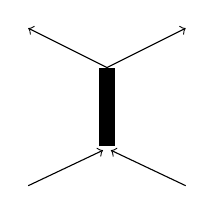
\begin{tikzpicture}[scale=0.5]
      \draw[->] (0,0) -- (1.9,0.9);
      \draw[->] (4,0) -- (2.1,0.9);
      \draw[->] (2,3) -- (0,4);
      \draw[->] (2,3) -- (4,4);
      \draw[line width=6pt] (2,1) -- (2,3);
    \end{tikzpicture}
\end{center}
  \caption{Planar graph with ``wide edge'' in matrix factorization for $sl{(N)}$ knot homology}
\end{figure}
This linear combination for each crossing is a \emph{resolution}.  To each resolution $\Gamma$, Khovanov and Rozansky associates a collection of matrix factorizations $M_1, \dots , M_m$, one for each of the crossings of $D$, with potentials $W_1, \dots , W_m$, such that they add up to zero: $W_1 + W_2 + \dots + W_m =0$.   The $W$'s cancel, so that $\mathcal{Q}$ becomes an ordinary differential, i.e. now $\mathcal{Q}^2=0$.  Also, the tensor product $M_1 \otimes M_2 \otimes \dots \otimes M_m$ becomes a two-periodic complex.   The result becomes the desired chain complex:
\begin{equation}
  \mathcal{C}^*_{n}{ (L)} = \otimes_i M_i
\end{equation}

 \section{Differentials for a colored superpolynomial}

To recap, for a knot $K$, the Jones polynomial $J(q)$ is the Euler characteristic of Khovanov homology $\text{Kh}{(q,t)}$.  $\text{Kh}{(q,t)}$ is its categorification:

\begin{align}
  & J(q) = \sum_{i,j} (-1)^i q^j \text{dim}{ \mathcal{H}_{i,j}{(K)} } \\
   & \text{Kh}{ (q,t)} = \sum_{i,j} t^i q^j \text{dim}{ \mathcal{H}_{i,j}{(K)} }
\end{align}

For a knot $K$, there also exists a homology theory categorifying the HOMFLY-PT polynomial $P{(a,q)}$. \cite{KhovanovRozansky2004}, \cite{KhovanovRozansky2005}   This theory is, as expected, to be triply graded, as the HOMFLY-PT polynomial is a 2-variable knot invariant.  Associate a Poincar\'{e} polynomial $\mathcal{P}{(a,q,t)}$ to the HOMFLY-PT homology.  The HOMFLY-PT polynomial is recovered as the Euler characteristic of this homology:
\begin{align}
  & P{(a,q)} = \sum_{ ijk} (-1)^k a^i q^j \text{dim}{ \mathcal{H}_{ijk}{(K) }} \\ 
  & \mathcal{P}{ (a,q,t)} = \sum_{ijk} a^i q^j t^k \text{dim}{ \mathcal{H}_{ijk}{(K)} }
\end{align}

\begin{figure}[h]
\begin{center}
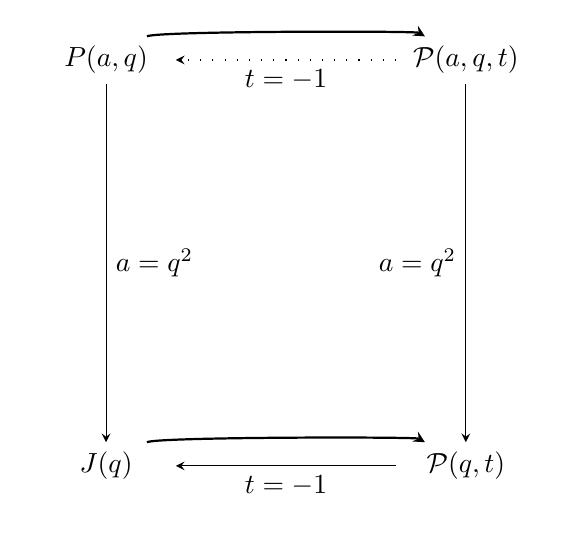
\begin{tikzpicture}
  \matrix (m) [matrix of math nodes, row sep=13em, column sep=8em, minimum width=5em]
  {
    P{ (a,q) }  &  \mathcal{P}{ (a,q,t) }  \\
    J{ (q) }  & \mathcal{P}{(q,t)}    \\ };
  \path[-stealth]
  (m-1-1) edge[thick,bend left, looseness = 0.1] (m-1-2)
  edge node [auto] {$a=q^2$} (m-2-1)
  (m-1-2) edge[loosely dotted] node [below] {$t=-1$} (m-1-1)
  edge node [left] { $a=q^2$} (m-2-2)
  (m-2-1) edge[thick,bend left, looseness = 0.1] (m-2-2)
  (m-2-2) edge node [below] {$t = -1 $} (m-2-1);
\end{tikzpicture} 
\end{center}
\caption{Categorification of the quantum knot invariants.   } \label{Fig:CatcoloredsuperPoly00}
\end{figure}

Thus, the relations between the polynomial and homological invariants are summarized diagramatically in Figure \ref{Fig:CatcoloredsuperPoly00}.  To the knot polynomial (respectively homological) invariants in Figure \ref{Fig:CatcoloredsuperPoly00}, there exists colored versions of the knot polynomials and homologies with either an associated group $sl{(2)}$ or $sl{(n)}$ in the fundamental representation $R$ of dimension $n$.    Let us decorate Figure \ref{Fig:CatcoloredsuperPoly00} with $R$ to emphasize this point. 


\begin{figure}[h]
\begin{center}
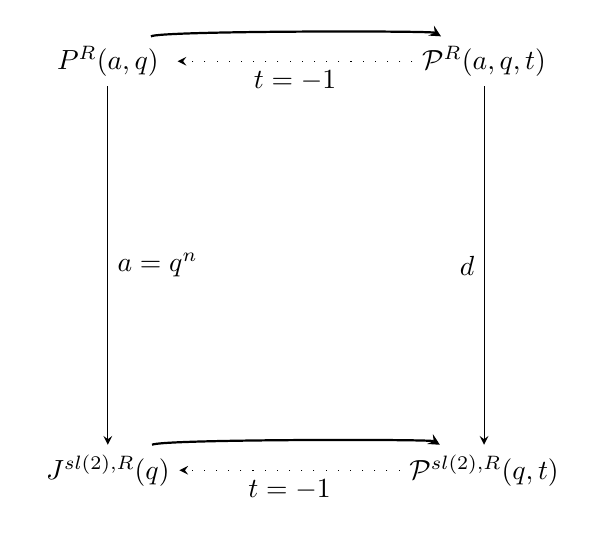
\begin{tikzpicture}
  \matrix (m) [matrix of math nodes, row sep=13em, column sep=8em, minimum width=5em]
  {
    P^R{ (a,q) }  &  \mathcal{P}^R{ (a,q,t) }  \\
    J^{ sl{(2)}, R }{ (q) }  & \mathcal{P}^{ sl{ (2)}, R }(q,t)    \\ };
  \path[-stealth]
  (m-1-1) edge[thick,bend left, looseness = 0.1] (m-1-2)
  edge node [auto] {$a=q^n$} (m-2-1)
  (m-1-2) edge[loosely dotted] node [below] {$t=-1$} (m-1-1)
  edge node [left] { $d$} (m-2-2)
  (m-2-1) edge[thick,bend left, looseness = 0.1] (m-2-2)
  (m-2-2) edge [loosely dotted] node [below] {$t = -1 $} (m-2-1);
\end{tikzpicture} 
\end{center}
\caption{Categorification of colored quantum knot invariants. Note that the polynomial (respectively homological) knot invariants which have the $a$-dependence (respectively $a$-grading) are \emph{not} labeled by $sl{(N)}$ } \label{Fig:CatcoloredsuperPoly01}
\end{figure}

%What ends up happening is that the $a$-grading or $t$ grading, or $a$ deformation or $t$ deformation, respectively, captures the information about the coloring by $\text{sl}{(2)}$ in its fundamental representation.


The process of decategorification corresponds to substituting in $t=-1$, in both uncolored and colored versions.  

The Poincar\'{e} polynomial that is the homological object categorifying the colored HOMFLY-PT knot polynomial is the \emph{colored superpolynomial} $\mathcal{P}^R{ (a,q,t)}$.  

For example, consider the trefoil knot, i.e. the torus knot $T^{(2,3)}$, and its colored Poincar\'{e} polynomial $\mathcal{P}_n{ (a,q,t)}$.  For $n=2$ (and note that the rank of the fundamental representation is $r=n-1=1$),  $\mathcal{P}_n{ (a,q,t)}$ is given by the following for the trefoil:

\begin{equation}
\mathcal{P}{ (a,q,t )} =   a^{2} t^{3} + a q t^{2} + \frac{a}{q} \label{Eq:coloredPtrefoilr01}
\end{equation}

Let $t=-1$.  Thus, in the Figure \ref{Fig:CatcoloredsuperPoly01}, we move to the left in a process called ``decategoritifaction.''  The HOMFLY-PT polynomial is recovered:

\[
\mathcal{P}{( a,q) }= -a^{2} + a q + \frac{a}{q}
\]

The Jones polynomial can be recovered by recalling that it is a  $\text{sl}{(2)}$ homological invariant, and so letting $a=q^2$, one recovers the following:

\[
J(q) = -q^{4} + q^{3} + q
\]


One could ask if one could follow the diagram in Figure \ref{Fig:CatcoloredsuperPoly01} the other way around, reversing all those steps immediately above.  Indeed, this is what categorification does.  

However, is there a way to recover the colored HOMFLY-PT homology, and obtain the colored superpolynomial $\mathcal{P}^R{(a,q,t)}$  directly from the Khovanov homology $\mathcal{P}^R{(q,t)}$?  For Figure \ref{Fig:CatcoloredsuperPoly01}, this would be going upwards from $\mathcal{P}^R{(q,t)}$ to $\mathcal{P}^R{(a,q,t)}$ on the right hand side.  This is a delicate issue.  First, the substitution of $a=q^2$ does not make sense in the context of the homology theories; $a$ is its own grading in the triply-graded homology theory.    

What ends up happening is that the correct lift involves a family of differentials $\lbrace d_N \rbrace$, \, $N \in \mathbb{Z}$.  After decategorification to the right hand side of Figure \ref{Fig:CatcoloredsuperPoly01}, no differentials are involved with the knot polynomial invariants; they do not play a role.  However, to relate different homologies, it turns out that differentials will have to play a role. 
% This has no analog at the (decategorified) polynomial level, i.e. the left side of Figure \ref{Fig:CatcoloredsuperPoly00} or Figure \ref{Fig:CatcoloredsuperPoly01}.  As seen before with Khovanov homology, $\mathcal{H}_*{ (K)}$ is to be equipped with this family of differentials $\lbrace d_N \rbrace$ for $N \in \mathbb{Z}$, which will give the different homologies.  

Dunfield, Gukov, and Rasmussen proposed the following axioms that the differentials $\lbrace d_N \rbrace$, $N \in \mathbb{Z}$, are to satisfy \cite{DunfieldGukovRasmussen2005}:

\begin{itemize}
  \item \textbf{Grading}: For $N \geq 0$, $d_N$ is triply graded of degree $( -1,N,-1)$, i.e.
\[
d_N: \mathcal{H}_{ i, j ,k }{ (K) } \to \mathcal{H}_{ i-1, j+N, k-1}{ (K) } 
\]

%$d_0$ is triply graded with $a,q,t$-grading degree $(-1,0,-1)$.  
For $N<0$, $d_N$ has degree $(-1,N, -3)$
\item \textbf{Anticommutativity}: $d_N d_M = -d_M d_N$, $\forall\, N, M \in \mathbb{Z}$.  In particular, $d^2_N =0$, $\forall \, N \in \mathbb{Z}$.  We have a homology.  
\item \textbf{Symmetry}: There is an involution $\phi: \mathcal{H}_{ i,j,* } \to \mathcal{H}_{i,-j,*}$ such that
\[
\phi d_N = d_{-N} \phi \quad \forall \, N \in \mathbb{Z}
\]
\end{itemize}
The homological lift of the colored Khovanov homology to the colored superpolynomials can now be done. 

For the differentials, note that in this work, the fundamental representation $R$ was exclusively employed, so that for gauge group $G=SU(N)$ and its complexification $G_{\mathbb{C}}=SL(N,\mathbb{C})$, the fundamental representation as a Young tableau of a single row of $n-1=r$ boxes, i.e. 
\[
R = \overbrace{ \yng(2) \dots \yng(2) }^{n-1}  \equiv S^{n-1}
\]
So the notation $n$ for the dimension of the fundamental representation and $r\equiv n-1$, for the rank of the symmetric representation, will be employed interchangeably, in this work, for the colored knot polynomials. 

%For the differentials, note that in this work, the fundamental representation $R$ was employed, so that for gauge group $G=SU(N)$ and its complexification $G_{\mathbb{C}}=SL(N,\mathbb{C})$ (or sometimes simply denoted $SL(n)$ in this work), the fundamental representation as a Young tableau of a single row of $n-1=r$ boxes, i.e. 



\subsection{Colored HOMFLY-PT homology}

The top half and right hand side of Figure \ref{Fig:CatcoloredsuperPoly01} will be explained.  A triply-graded homology theory for the colored reduced HOMFLY-PT polynomials will come with differentials.  Not only will it come with the family of differentials $\lbrace d_N^{S^r}\rbrace$ with $N \in \mathbb{Z}$, but it will also come with an additional collection of \emph{universal colored} differentials $d_{n\to m}$, for all $1 \leq m < n \leq r$ that relates homologies of differential symmetric representations.  

The following is the main conjecture and properties of such a triply-graded homology theory proposed by Gukov and Sto\v{s}i\'{c} \cite{GukovStosic2012}:

\begin{itemize}
\item \textbf{Categorification}: $\mathcal{H}^{S^r}_*$ categorifies $P^{S^r}$

\[
\chi{ (\mathcal{H}^{ S^r}_*{ (K) }) } = P^{ S^r}{ (K) }
\]
\item \textbf{ Anticommutativity}: The family of differentials $\lbrace d_N^{ S^r} \rbrace$, $\forall \, N \in \mathbb{Z}$  anticommute:

\[
d^{S^r}_N d^{S^r}_M = - d^{S^r}_M d^{S^r}_N
\]
$\forall \, M,N \in \mathbb{Z}$.  Note that for $M=N$, $d^2=0$.  
\item \textbf{Finite support}:
\[
\text{dim}{ (\mathcal{H}_*^{ S^r} ) } < + \infty
\]

\item \textbf{Specializations}: For $N >1$, the homology of $\mathcal{H}^{ S^r}{ (K)}$ with respect to $d^{S^r}_N$ is isomorphic to $\mathcal{H}^{ \text{sl}{(N)}, S^r}{ (K)}$: 

\[
\left( \mathcal{H}_*^{S^r}{ (K)}, d_N^{S^r}  \right) \cong \mathcal{H}^{ \text{sl}{ (N)}, S^r}{ (K)}
\]
\item \textbf{Canceling differentials}: Differentials $d_1^{S^r}$ and $d^{S^r}_{-r}$ are \emph{canceling}: the homology groups $\mathcal{H}^{ S^r}_*{ (K)}$ with respect to the differentials $d_1^{S^r}$ and $d^{S^r}_{-r}$ is one-dimensional.  The gradings of the remaining generators are simple invariants of the knot $K$.  
\item \textbf{Vertical Colored differentials}: There are differentials $d^{S^r}_{1-k}$, for $1 \leq k \leq r-1$, with $a$-degree $-1$.  The homology groups $\mathcal{H}_*^{ S^r}{ (K) }$ with respect to the differential $d^{S^r}_{ 1-k}$ is isomorphic, after simple regrading that preserves $a$- and $t$-gradings, to the $k$-colored homology $\mathcal{H}_*^{S^k}{ (K)}$, i.e.
\[
\left( \mathcal{H}_*^{S^r}{ (K) } , d^{S^r}_{ 1-k } \right) \cong \mathcal{H}_*^{ S^k}{ (K)} 
\]
\item \textbf{Universal Colored differentials}: For every positive integer $m$, with $m<r$, the differentials $d_{r\to m}$ have $a$-degree $0$, and the homology groups $\mathcal{H}_*^{S^r}{(K)}$ with respect to the colored differential $d_{r\to m}$ is isomorphic (after regrading) to the $m$-colored homology $\mathcal{H}_*^{S^m}{ (K)}$:
\[
\left( \mathcal{H}_*^{ S^r}{ (K)}, d_{r\to m} \right) \simeq \mathcal{H}_*^{S^m}{ (K)}
\]
\end{itemize}

\subsubsection{Size of the homology}

It was conjectured in \cite{GukovStosic2012}, from examining explicit computations, that for a knot $K$, the rank of the homology $\mathcal{H}^{S^r}$ grows exponentially with $r$.  Precisely, what this means is the following:



\begin{equation}
  \text{rank}{ \mathcal{H}^{S^r}{(K)} } = \left( \text{rank}{ \mathcal{H}^S{ (K) } } \right)^r
\end{equation}

Note that for all the knots considered in this work, the torus knots and twist knots, the knots are ``homologically thin.''  Knots that are homologically thin are knots with homologies that are free $R$-modules,  supported in only one, overall, ``$\delta$''-grading: for instance, taking $\delta = j-i$, where $i,j$ are the gradings for $a$ and $q$ in the homology, respectively.  One version of the definition of a homologically thin knot appeared in \cite{Bar-Natan2002}, namely in the conjectures.  It was proven that alternating knots, such as the torus and twist knots considered here in this work are homologically thin; see \cite{Lee2002}.  Nevertheless, torus and twist knots are conjectured to satisfy a refined exponential growth conjecture \cite{FujiGukovStosicSulkowski2013}:

\begin{equation}
  \mathcal{P}^{S^r}{(a,q=1,t) } = ( \mathcal{P}^{S}{ (a,q=1,t) }   )^r \label{Eq:refinedexponentialgrowth}
\end{equation}

In the following, further elaborations and applications of the various differentials previously mentioned will be provided.

\subsubsection{$d_N$ differentials}\label{subsubsec:differentialsfamily}

The family of differentials $\lbrace d_N \rbrace$ is indexed by $N$ that ranges from $-2n+3, \dots , 1$.  

In the $n$-colored HOMFLY-PT homology, $d_{2-n}$ differential provides the relation to knot Floer homology \cite{DunfieldGukovRasmussen2005}.  The action of this differential can be deduced from the expression for $\mathcal{P}_n{(a,q,t)}$.  

\subsubsection{Canceling differentials}

With respect to a canceling differential, the knot homology  is ``trivial'' and so it would be isomorphic to the homology of the unknot.  For the \emph{reduced} theory, this means that the resulting homology is one-dimensional.  For knot polynomials, one should obtain a monomial.

The degrees of the canceling differentials of the colored HOMFLY-PT homology $\mathcal{H}^{S^r}$, $d_1^{S^r}$ and $d^{S^r}_{-r}$ are the following:

\[
\begin{aligned}
  & \text{deg}{ (d_1^{S^r}) } = ( -1, 1, -1 ) \\ 
  & \text{deg}{ (d_{-r}^{S^r} ) } = (-1,-r,-3)
\end{aligned}
\]



\subsubsection{Vertical Colored differentials}

In the case for these $S^r$-colored triply-graded HOMFLY-PT homologies $\mathcal{H}^{S^r}{ (K)}$, there exists the \emph{colored} differentials, that are a family of differentials, but for different values of $r$ \cite{GukovStosic2012}.  For a given knot $K$, and for every $k=0 \dots r-1$, there exists differential $d_{1-k}$ on $\mathcal{H}^{ S^r}{ (K)}$ of $(a,q,t)$-degree $(-1,1-k,-1)$.  
\begin{equation}
  \text{deg}{ (d^{S^r}_{1-k}) } = (-1,1-k, -1), \quad \, 1 \leq k \leq r-1
\end{equation}
These differentials are called \emph{vertical colored differentials}.  

For $r=2$, there is one vertical colored differential, $d_0^{S^2}$ of $a,q,t$-grading $(-1,0,-1)$.  

\subsubsection{Examples}




To illustrate differentials, it is convenient to represent $\mathcal{H}{(K)}$ by a \emph{dot diagram}. One dot is drawn for each term in the superpolynomial.  The total number of dots is equal to the dimension of $\mathcal{H}{(K)}$.  The horizontal axis runs over the exponential powers of $q$, and the vertical axis runs over the exponential powers of $a$.  The trefoil has two nontrivial differentials: $d_1$ and $d_{-1}$.  

\begin{figure}[h]
\begin{center}
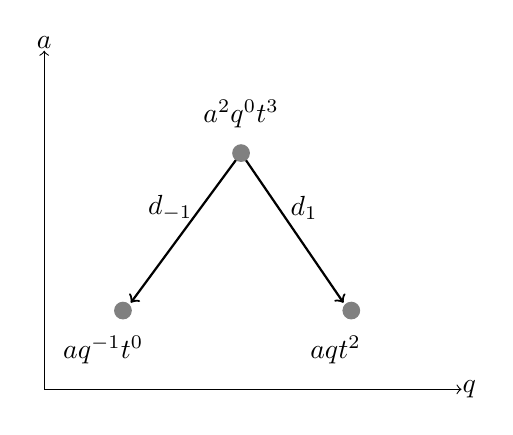
\begin{tikzpicture}
  \draw[->] (0,0) -- (5.3,0);   % horizontal axis for q
  \draw[->] (0,0) -- (0,4.3);   % vertical axis for a
  \draw[->,thick] (2.5,3) -- (1.1,1.1);   % diagonal line down and to the left for d_{-1} 
  \draw[->,thick] (2.5,3) -- (3.8,1.1);   % diagonal line down and to the right for d_{1} 
  \filldraw [gray] (2.5,3) circle (3pt);  % dots, top dot
  \filldraw [gray] (1,1) circle (3pt);  % left bottom dot
  \filldraw [gray] (3.9,1) circle (3pt); % right bottom dot
  \draw (5.4,0) node {$q$};  % labels
  \draw (0,4.4) node {$a$};
  \draw (1.6,2.3) node {$d_{-1}$};
  \draw (3.3,2.3) node {$d_{1}$}; 
  \draw (2.5,3.5) node {$a^2 q^0 t^3$ }; 
  \draw (0.75,0.5) node {$aq^{-1}t^0$ };
  \draw (3.7, 0.5) node {$a q t^2$};
\end{tikzpicture}   \quad \quad \quad 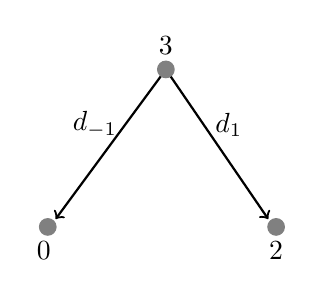
\begin{tikzpicture}
  \draw[->,thick] (2.5,3) -- (1.1,1.1);   % diagonal line down and to the left for d_{-1} 
  \draw[->,thick] (2.5,3) -- (3.8,1.1);   % diagonal line down and to the right for d_{1} 
  \filldraw [gray] (2.5,3) circle (3pt);  % dots, top dot
  \filldraw [gray] (1,1) circle (3pt);  % left bottom dot
  \filldraw [gray] (3.9,1) circle (3pt); % right bottom dot
  \draw (1.6,2.3) node {$d_{-1}$};
  \draw (3.3,2.3) node {$d_{1}$}; 
  \draw (2.5,3.3) node {$3$ }; 
  \draw (0.95,0.7) node {$0$ };
  \draw (3.9, 0.7) node {$2$};
\end{tikzpicture}   
\end{center}
\caption{Differentials for the trefoil knot.  The diagram on the right is the same as the left, but in a condensed and abbreviated form.}\label{Fig:dotdiagramtrefoilr01}
\end{figure}

According to the discussion on the family of differentials $\lbrace d_N \rbrace$ above, \ref{subsubsec:differentialsfamily}, in this uncolored theory for $n=2$, there are only three differentials for $\lbrace d_N \rbrace$: $d_{\pm 1}$ and $d_{0}$.  $d^{\pm 1}$ are the canceling differentials.  $d_0$ is the differential that relates HOMFLY-PY homology to  knot Floer homology (informally, knot Floer homology maps cycles on a symplectic manifold to a homology)  \cite{DunfieldGukovRasmussen2005}.  $d_0$ is not exhibited in the uncolored Poincar\'{e} polynomial $\mathcal{P}{(a,q,t)}$.  However, how $d_0$ acts on HOMFLY-PT homology is contained in the colored versions of the HOMFLY-PT homology, encapsulated in $\mathcal{P}_n{(a,q,t)}$.  


Take the $\text{sl}{ (1)}$ homology, so that $N=1$, i.e. $r=0$.  But $\text{sl}{(1)}$ homology is just one-dimensional (trivial)!  One should reobtain a monomial.  

Substitute $a=q^n$ into (\ref{Eq:coloredPtrefoilr01}).  One obtains
\[
\mathcal{P}_n{(q,t)} = q^{2n} t^3 + q^{n+1}t^2 + q^{n-1}
\]
There are no differentials for $N>1$.  For $n=1$, and then $t=-1$, $\mathcal{P}_1 =1$ for the trefoil.  

Indeed, consider this factorization of (\ref{Eq:coloredPtrefoilr01}):

\[
\mathcal{P}{(a,q,t)} = aq^{-1}( 1 + ( 1 + a^{-1}q t^{-1})aqt^3 )
\]

Disregarding the overall multiplicative factor of $aq^{-1}$, notice the factor of $(1+a^{-1}qt^{-1})$.  When $t=-1$, the factor becomes zero in the $\text{sl}{(1)}$ homology.  Think of the differential $d_1$.  It has a definite $(a,q,t)$-grading of $(-1,1,-1)$. Differential $d_1$ leaves behind a ``trivial'' one-dimensional space
\[
\text{dim}{ (\mathcal{H}_*, d_1)} = 1
\]
and so $\mathcal{P}{(a,q,t)}$ must be of the following general form:

\begin{equation}
  \mathcal{P}{ (a,q,t)} = 1 + ( 1 + a^{-1} qt^{-1})Q_+{ (a,q,t)}
\end{equation}
where the first term, $1$, represents the contribution of the (trivial) $\text{sl}{ (1)}$ knot homology, and $Q_+{ (a,q,t)}$ is some polynomial with positive coefficients.

Now consider $\mathcal{P}^{S^r}{ (a,q,t)}$ for the same trefoil, $K = \mathbf{3}_1$, but now colored by $r=2$, $S^2$ symmetric representation, i.e. $\mathcal{P}^{S^2}$, given by the following:

\begin{equation}
  \mathcal{P}^{ S^2  }{ (a,q,t) }  =   a^{4} q^{3} t^{6} + {a^3 \left( q^{4} +  q^{3}\right)} t^{5} + a^{2} q^{4} t^{4}  + {\left(a^{3} q + a^{3}\right)} t^{3} + {\left(a^{2} q^{2} + a^{2} q\right)} t^{2} + \frac{a^{2}}{q^{2}} \label{Eq:coloredPtrefoilr02}
\end{equation}


\begin{figure}[h]
\begin{center}
  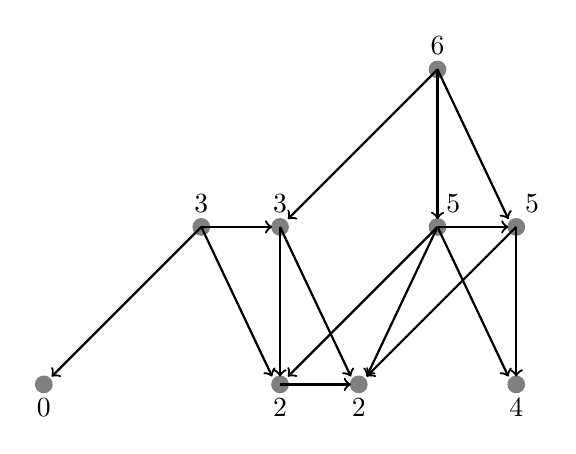
\begin{tikzpicture}
    \filldraw [gray] (3,6) circle (3pt)  % dots, starting from the top, and then starting from the left, across a row
    (0,4) circle (3pt)
    (1,4) circle (3pt)
    (3,4) circle (3pt)
    (4,4) circle (3pt)
    (-2,2) circle (3pt)
    (1,2) circle (3pt)
    (2,2) circle (3pt)
    (4,2) circle (3pt);
%    \draw[->,thick] (3,6) -- ( 0.1,4.1 );  % diagonals for the differentials
    \draw[->,thick] (3,6) -- ( 1.1 , 4.1); 
 \draw[->,thick]    (3,6) -- (3, 4.1);
\draw[->,thick]    (3,6) -- (3.9, 4.1);
    \draw[->,thick] (0,4) -- (-1.9,2.1) ;
     \draw[->,thick] (0,4) -- (0.9,2.1);
%    \draw[->,thick] (1,4) -- (-1.9,2.1);
    \draw[->,thick] (1,4) -- (1,2.1);
    \draw[->,thick] (1,4) -- (1.9,2.1);
    \draw[->,thick] (3,4) -- (1.1,2.1);
    \draw[->,thick] (3,4) -- (2.1,2.1);
    \draw[->,thick] (3,4) -- (3.9,2.1);
%    \draw[->,thick] (4,4) -- (1.1,2.1);
    \draw[->,thick] (4,4) -- (2.1,2.1);
    \draw[->,thick] (4,4) -- (4,2.1);
    \draw[->,thick] (0,4) -- (0.9,4);
    \draw[->,thick] (3,4) -- (3.9,4);
    \draw[->,thick] (1,2) -- (1.9,2);
\draw (3,6.3) node {$6$};
\draw (0,4.3) node {$3$};
\draw (1,4.3) node {$3$};
\draw (3.2,4.3) node {$5$};
\draw (4.2,4.3) node {$5$};
\draw (-2,1.7) node {$0$};
\draw (1,1.7) node {$2$};
\draw (2,1.7) node {$2$};
\draw (4,1.7) node {$4$};
\end{tikzpicture}
\end{center}
\caption{Dot diagram for the trefoil knot in the $S^2$, $r=2$ symmetric representation of the superpolynomial $\mathcal{P}{  (a,q,t)  }$ } \label{Fig:dotdiagramtrefoilr02}
\end{figure}

Figure \ref{Fig:dotdiagramtrefoilr02} is the dot diagram for $\mathcal{P}^{ S^2  }{ (a,q,t) }$ with $K=\mathbf{3}_1$, the trefoil. There are 9 dots and thus the dimension is 9.  


The axioms, such as the anticommutativity axiom, in that $d^2 =0$, are illustrated vividly in Figure \ref{Fig:dotdiagramtrefoilr02}.  From $d^2=0$, there are no two successive differentials.  Also, anticommutativity $d_N d_M = -d_Md_N$ for $N\neq M$ is made clear: for example, the term in $\mathcal{P}^{ S^2  }$, $a^2 q t^2$ can be reached via the differentials $d_0 d_{-2} = -d_{-2}d_0$ through the terms $a^3qt^3$ and $a^3q^3t^5$, respectively, from the term $a^4 q^3 t^6$.  Another example is that  $a^2 q^4 t^4$ can be reached via the differentials $d_0 d_1 = -d_1 d_0$, through the terms $a^3q^4t^5$ and $a^3 q^3t^5$ respectively, from the term $a^4 q^3 t^6$.

It should also be noted that for Figure \ref{Fig:dotdiagramtrefoilr02}, the various differentials with $(a,q,t)$-grading degrees are manifest:

\begin{itemize}
\item Two canceling differentials, $d_1^{S^2}$ and $d_{-2}^{S^2}$ have the following $(a,q,t)$-grading degrees:
\[
\begin{aligned}
  & \text{deg}{ (d_1^{S^2}) } = (-1,1,-1) \\
  &  \text{deg}{ (d_{-2}^{S^2} ) } = (-1,-2,-3)
\end{aligned}
\]
\item The so-called vertical colored differential $d_0^{S^2}$ is observed, and has degree $(-1,0,1)$
\item The so-called universal colored differential $d_{2\to 1}$ has degree $(0,1,0)$
\end{itemize}



Now let $q=1$ in (\ref{Eq:coloredPtrefoilr02}) for $\mathcal{P}^{S^2}$.  

\begin{equation}
  \mathcal{P}^{S^2}{ (a,q=1,t) } = a^{4} t^{6} + 2 \, a^{3} t^{5} + 2 \, a^{3} t^{3} + a^{2} t^{4} + 2 \, a^{2} t^{2} + a^{2} = {\left( ( a t +  1) t^{2} + 1\right)}^{2} a^{2}
\end{equation}

Let $q=1$ in (\ref{Eq:coloredPtrefoilr01}) for $\mathcal{P}^{S^1}$.  

\begin{equation}
  \mathcal{P}^{S^1}{ (a,q=1,t) } = {\left( ( a t +  1 ) t^{2} + 1\right)} a
\end{equation}

%Remember that the vertical colored differential $d_0^{S^2}$ is of $(a,q,t)$-grading degree of $(-1,0,-1)$, yielding a factor $(1+a^{-1}t^{-1})$, or $a^{-1}t^{-1}(1+at)$.  

This confirms (\ref{Eq:refinedexponentialgrowth}) for the HOMFLY-PT homology for the trefoil, in the case of the symmetric representation $r=2$.  %Note that there is only $k=1$.  
\[
\mathcal{P}^{S^2}_{\mathbf{3}_1}{ (a,q=1,t) } = ( \mathcal{P}^S_{\mathbf{3}_1}{ (a,q=1,t)} )^2
\]


Now, examining (\ref{Eq:coloredPtrefoilr01}) and (\ref{Eq:coloredPtrefoilr02}), and Figure \ref{Fig:dotdiagramtrefoilr01} and Figure \ref{Fig:dotdiagramtrefoilr02}, could one go from one Young tableau representation to another, even in the case of this symmetric representation?  Indeed, a family of \emph{colored differentials} was constructed \cite{GukovStosic2012} which act by removing boxes from the Young tableau representation, reducing the dimension of the representation coloring the knot diagram.  In other words,

\begin{equation}
  ( \mathcal{H}^{  S^2 }, d_{\text{colored}}) \simeq \mathcal{H}^{  S^1 } 
\end{equation}
where $(\mathcal{H}^{  S^2 }, d_{\text{colored}})$ denote the homology with respect to the differential $d_{\text{colored}}$.  This is expressed for the colored superpolynomials $\mathcal{P}^{S^r}{(a,q,t)}$ as a relation of the following form:


\begin{equation}
  \mathcal{P}^{ S^2   }{ (a,q,t) } = a^{s} \mathcal{P}^{ S^1   }{ (a,q^2, t)} + (1+at) Q_+{ (a,q,t)}
\end{equation}


Thus, for the trefoil, indeed, $\mathcal{P}^{S^2}{(a,q,t)}$ can be factored into the following form:



\begin{equation}
  \mathcal{P}^{ S^2   }{ (a,q,t) } = a \mathcal{P}^{ S^1     }{ (a,q^2,t)} + ( 1 + at) Q_+{ (a,q,t)}
\end{equation}
with 
\[
Q_+{(a,q,t)} = {\left( ( aq^{-1} t  + 1 ) q^3 t^2  + 1\right)}  a^{2} q t^{2}
\]

This $d_{\text{colored}}$ differential has $(a,q,t)$-grading $(1,0,1)$.  

Consider the family of torus knots $T^{(2,2p+1)}$, starting from $p=1$.  Consider the cinquefoil, $\mathbf{5}_1$, a torus knot, such that $p=2$.  


\begin{figure}[h]

   \begin{center} 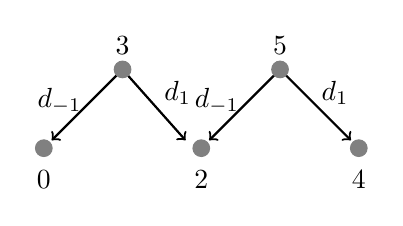
\begin{tikzpicture}
  \draw[->,thick] (1,1) -- (0.1,0.1);   % diagonal line down and to the left for d_{-1} 
  \draw[->,thick] (1,1) -- (1.8,0.1);   % diagonal line down and to the right for d_{1} 
  \draw[->,thick] (3,1) -- (2.1,0.1);
  \draw[->, thick] (3,1) -- (3.9, 0.1);
  \filldraw [gray] (0,0) circle (3pt);  % dots, left dot
  \filldraw [gray] (1,1) circle (3pt);  % 2nd left top dot
  \filldraw [gray] (2,0) circle (3pt); % 3rd left bottom dot
  \filldraw [gray] (3,1) circle (3pt)
  (4,0) circle (3pt);
  \draw (0.2,0.6) node {$d_{-1}$};
  \draw (1.7,0.7) node {$d_{1}$}; 
  \draw (2.2,0.6) node {$d_{-1}$};
  \draw (3.7,0.7) node {$d_1$};
  \draw (1.0,1.3) node {$3$ }; 
  \draw (0.0,-0.4) node {$0$ };
  \draw (2.0, -0.4) node {$2$};
  \draw (3.0, 1.3) node {$5$};
  \draw (4.0, -0.4) node {$4$};
\end{tikzpicture}   
\end{center}
\caption{Dot diagram for the cinquefoil knot in the $S^1$, $r=1$ symmetric representation of the superpolynomial $\mathcal{P}{  (a,q,t)  }$ } \label{Fig:dotdiagramcinquefoilr01}
\end{figure}

Figure \ref{Fig:dotdiagramcinquefoilr01} is the dot diagram for the cinquefoil.  The nontrivial differentials are $d_{-1}$ and $d_1$.  For a given symmetric representation, one could speculate on a relationship across the family of torus knots, starting from $p=1$.  Indeed, this is the case, as shown in \cite{DunfieldGukovRasmussen2005}.      If one speculates on a further ``$\delta$-grading'', given by an expression for the $(a,q,t)$ grading of the form $j - 2i -k$, then note that only for $d_1$, $d_{-1}$ differentials does one have that the values for $j-2i-k$ are $-1 - 2(-1) -(1) =0$ and $-3 - 2(-1) - (-1) = 0$, respectively.   $d_1$ and $d_{-1}$ are the only nontrivial differentials.

From both Figure \ref{Fig:dotdiagramtrefoilr01} and Figure \ref{Fig:dotdiagramcinquefoilr01}, the symmetry property mentioned in the axioms is exhibited the symmetry about the vertical $a$ axis, ``flipping'' across the $q$-axis.

\begin{figure}[h]
  \begin{center}
    \begin{tabular}{l c r }
      differentials & factors & $(a,q,t)$ grading \\
      \hline
      $d_{N >0 }$           &  $ 1 +  aq^{-N}t  $  & $ ( -1 , N , -1 ) $ \\
      $d_{N<0} $            &  $ 1 + aq^{-N} t^3 $ & $ (-1 , N , -3 )  $ \\ 
      $d_{\text{colored} }$ &  $ 1 + q $           & $ ( 0, 1, 0 ) $     \\
                            &  $ 1 + at $          & $ ( -1, 0 , -1 )$   \\
%                            & $\vdots $            &
      \end{tabular}
  \end{center} 
\caption{Differentials in knot homologies} \label{Fig:differentialschart}
\end{figure}

%Figure \ref{Fig:differentialschart} tabulates some of these differentials and the $(a,q,t)$-degrees.  
The factors of the form $(1 + a^i q^j t^k)$ come from differentials of $(a,q,t)$-degree $(i,j,k)$ The factors and associated differentials and the gradings of the degrees are recounted in Figure \ref{Fig:differentialschart}.

\subsubsection{Homological lift by a differential} \label{subsubsec:homoliftviadiff}

Finally, let us come back to the trouble of homologically lifting the categorified colored Jones polynomial, $\mathcal{P}^{sl{(2)},R}{(q,t)}$ to the colored superpolynomial, $\mathcal{P}^R{(a,q,t)}$, i.e. the right hand side of Figure \ref{Fig:CatcoloredsuperPoly01}.  The two homology theories are related by a certain differential \cite{GukovStosic2012}, which at the level of Poincar\'{e} polynomials implies the relation
\begin{equation}
\mathcal{P}_n{(a,q,t)} = R_n{(a,q,t)} + (1+a^{-1} q^2 t^{-1})Q_n{(a,q,t)}  \label{eq:diffbetweenhomo00}
\end{equation}
where $R_n{(a,q,t)}$ and $Q_n{(a,q,t)}$ are polynomials with non-negative coefficients, such that $\mathcal{P}^{ sl{(n)},R}{ (q,t)} = R_n{(q^2, q,t)}$.  This differential, with $a,q,t$-grading $(-1,2,-1)$, acts nontrivially.  
%Also note that it belongs to the family of differentials, $\lbrace d_N \rbrace$, described in \ref{subsubsec:differentialsfamily}.  


\begin{figure}[h]
\begin{center}
  \begin{tikzpicture}
    \filldraw [gray] (3,6) circle (3pt)  % dots, starting from the top, and then starting from the left, across a row
    (0,4) circle (3pt)
    (1,4) circle (3pt)
    (3,4) circle (3pt)
    (4,4) circle (3pt)
    (-2,2) circle (3pt)
    (1,2) circle (3pt)
    (2,2) circle (3pt)
    (4,2) circle (3pt);
    \draw[->,thick] (0,4) -- (1.9,2.1) ;
\draw (3,6.3) node {$6$};
\draw (0,4.3) node {$3$};
\draw (1,4.3) node {$3$};
\draw (3.2,4.3) node {$5$};
\draw (4.2,4.3) node {$5$};
\draw (-2,1.7) node {$0$};
\draw (1,1.7) node {$2$};
\draw (2,1.7) node {$2$};
\draw (4,1.7) node {$4$};
\end{tikzpicture}
\end{center}
\caption{Dot diagram for the trefoil knot in the $S^2$, $r=2$ symmetric representation of the superpolynomial $\mathcal{P}{(a,q,t)}$, highlighting the differential $d_2$ for $(a,q,t)$-grading $(-1,2,-1)$} \label{Fig:dotdiagramtrefoilr03}
\end{figure}

Consider once again the example of the trefoil, for $r=2$.  From the dot diagram, it is easy to identity the differential $d_2$ with $(-1,2,-1)$ $a,q,t$-grading; see Figure \ref{Fig:dotdiagramtrefoilr03}.  Indeed, the colored superpolynomial $\mathcal{P}_2$ for this example can be put into this form:

\begin{equation}
  \mathcal{P}_2{(a,q,t)} = R_2{(a,q,t)} + ( 1 + a^{-1} q^2 t^{-1}) Q_2{(a,q,t)}
\end{equation}
with 
\begin{equation}
  \begin{aligned}
    R_2{(a,q,t)} & = \frac{a^{4} q^{5} t^{6} + a^{2} q^{6} t^{4} + a^{3} q^{3} t^{3} + a^{2} q^{3} t^{2} + {\left(a^{3} q^{6} + a^{3} q^{5}\right)} t^{5} + a^{2}}{q^{2}}    \\
    Q_2{(a,q,t)} & = a^3 t^3
  \end{aligned}
\end{equation}

Now specialize $R_2{(a,q,t)}$ for $a=q^2$: one reobtains the categorified colored Jones polynomial!
\begin{equation}
\begin{aligned}
  R_2{(q^2, q, t)} & = \mathcal{P}^{ sl{(2)},S^2}{(q,t)} = \\
  & = q^{11} t^{6} + q^{10} t^{5} + q^{9} t^{5} + q^{8} t^{4} + q^{7} t^{3} + q^{5} t^{2} + q^{2}
\end{aligned}
\end{equation}

Notice that for the differential $d_2$ with factor $(1 + a^{-1}q^2 t^{-1})$, the specialization $a=q^2$ leads to a factor $(1+t^{-1})$.  

\begin{equation}
\mathcal{P}_2{(a=q^2,q,t)} = \mathcal{P}^{sl{(2)}, S^2}{(q,t)} + ( 1 + t^{-1}) Q_2{(a=q^2, q,t)} \label{eq:trefoild2relation}
\end{equation}
In \eqref{eq:trefoild2relation}, only when $t=-1$ does one have a simple rule for decategorification, as the factor $(1+t^{-1})$ becomes zero, leaving the decategorified $\mathcal{P}^{sl{(2)},S^2}{(q,t)}$, the colored Jones polynomial.   

  




\subsection{Torus knots $T^{2,2p+1}$}

Due to constraints from such an analysis of the differentials in the respective homology theory, \cite{FujiGukovStosicSulkowski2013}, one is led to the following form for the colored superpolynomial $\mathcal{P}^{S^r}$ for the torus knot $T^{2,2p+1}$:

\begin{equation}
  \begin{gathered}
    \mathcal{P}^{ S^r}{ (T^{2,2p+1};a,q,t) } = a^{pr} q^{-pr} \sum_{ 0 \leq k_p \leq \dots \leq k_2 \leq k_1 \leq r} { r \brack k_1 } { k_1 \brack k_2 } \dots { k_{p-1} \brack k_p } \times \\
    \times q^{ (2r+1)( k_1 + k_2 + \dots + k_p )  - \sum_{i=1}^p k_{i-1} k_i } t^{ 2 (k_1 + k_2 + \dots + k_p ) } \prod_{i=1}^{ k_1} ( 1 - aq^{ i- 2 } t ) 
\end{gathered} \label{Eq:analysisofdtorusknotPr00}
\end{equation}

where $k_0 =r$.  Noting that, by definition of the $q$-Pochhammer symbol, 
\[
\prod_{i=1}^{k_1} (1 + a q^{i-2} t) = \left( \frac{-at}{q}, q \right)_k
\]
the above expression (\ref{Eq:analysisofdtorusknotPr00}) for $\mathcal{P}^{S^r}$ is rewritten as the following:

\begin{equation}
  \begin{gathered}
    \mathcal{P}^{ S^r}{ (T^{2,2p+1};a,q,t) } = a^{pr} q^{-pr} \sum_{ 0 \leq k_p \leq \dots \leq k_2 \leq k_1 \leq r} { r \brack k_1 } { k_1 \brack k_2 } \dots { k_{p-1} \brack k_p } \times \\
    \times q^{ (2r+1)( k_1 + k_2 + \dots + k_p )  - \sum_{i=1}^p k_{i-1} k_i } t^{ 2 (k_1 + k_2 + \dots + k_p ) } \left( -\frac{at}{q}, q \right)_{k_1}
\end{gathered} \label{Eq:analysisofdtorusknotPr01}
\end{equation}
which is used for computation in this work.  

For instance, for the case of the trefoil, $\mathcal{P}^{S^r}{(a,q,t)}$ becomes the following:
\begin{equation}
\mathcal{P}^{S^r}{ ( T^{(2,3)} ; a , q,t ) } = a^r q^{r^2} t^{2r} \sum_{k=0}^r { r \brack k } q^{ -(r+1)k } t^{-2k } \cdot \prod_{i=1}^k  \left( - \frac{at}{q} , q \right)_k \label{Eq:analysisofdifftrefoil} 
\end{equation}


\subsection{Twist knots, $TK_{2n+2}$}

By an analysis of the differentials and how they constrain the form of the colored superpolynomial, by generalizing the colored superpolynomial for the knots $\mathbf{4}_1$ and $\mathbf{6}_1$, the first two knots in a family of twist knots with even number of crossings, the $S^r$ colored homology, or colored superpolynomial, of the twist knot with $2n+2$ crossings, denoted by $TK_{2n+2}$, was calculated \cite{FujiGukovStosicSulkowski2013}:

\begin{equation}
\begin{gathered}
\mathcal{P}^{ S^r}_{TK_{2n+2} }{ (a,q,t)} = \sum_{ 0 \leq k_n \leq \dots \leq k_2 \leq k_1 \leq r} { r \brack k_1 } { k_1 \brack k_2 } \dots { k_{n-1} \brack k_n } \times \\
\times a^{ \sum_{i=1}^n k_i } q^{ \sum_{i=1}^n (k_i^2- k_i) } t^{ 2 \sum_{i=1}^n k_i } \prod_{i=1}^{k_1} (1 + a^{-1} q^{2-i } t^{-1} )(1 + a^{-1} q^{1-r-i} t^{-3} ) 
\end{gathered} \label{Eq:TwistKcoloredsuperpolynomial00}
\end{equation}

The above expression (\ref{Eq:TwistKcoloredsuperpolynomial00}) can be rewritten with the definition of $q$-Pochhammer symbol as the following:

\begin{equation}
\begin{gathered}
\mathcal{P}^{ S^r}_{TK_{2n+2} }{ (a,q,t)} = \sum_{ 0 \leq k_n \leq \dots \leq k_2 \leq k_1 \leq r} { r \brack k_1 } { k_1 \brack k_2 } \dots { k_{n-1} \brack k_n } \times \\
\times a^{ \sum_{i=1}^n k_i } q^{ \sum_{i=1}^n (k_i^2- k_i) } t^{ 2 \sum_{i=1}^n k_i } \left( \frac{-q}{ at} , q^{-1} \right)_{k_1} \left( \frac{-1}{ aq^r t^3 } , q^{-1} \right)_{ k_1} 
\end{gathered} \label{Eq:TwistKcoloredsuperpolynomial01}
\end{equation}
which is used for computation in this work.  

For example, the formula for the figure-eight knot is the following:

\begin{equation}
\mathcal{P}^{S^r}_{\mathbf{4}_1}{ (a,q,t)} = \sum_{k=0}^r { r \brack k }a^k q^{k^2 - k } t^{2k} \left( \frac{-q}{ at}, q^{-1} \right)_k \left( \frac{-1}{ aq^r t^3 }, q^{-1} \right)_k
\end{equation}

\subsection{Twist knot of odd number of crossings: $\mathbf{5}_1$}

The expression for the Poincar\'{e} polynomial of the $S^r$-colored HOMFLY-PT homology for the $\mathbf{5}_2$ knot, a twist knot of 5 crossings is the following \cite{FujiGukovStosicSulkowski2013}:

\begin{equation}
  \mathcal{P}^{S^r}_{\mathbf{5}_2}{ (a,q,t)} = a^r q^{-r} \sum_{ 0 \leq l \leq j \leq r} { r \brack j} { j \brack l } a^l q^{ l^2 - l + j(r+1) } t^{2j + 2l} (-aq^{-1}t;q)_j ( -q^{l-r}t^{-1};q)_{j-l}  \label{Eq:5_2coloredsuperpolynomial00}
\end{equation}

\chapter{Quantization} \label{chap:Quantization}

What is meant by quantization in the context of this work is discussed.  \cite{DimofteGukov2010} reviews quantization in relation to the volume conjectures, and \cite{GukovSaberi2012} provides a very pedagogically friendly explanation of quantization.  It will turn out that the exact solution to $SL{(2,\mathbb{C})}$ Chern-Simons theory, with Wilson loops, as mentioned in Chapter \ref{chap:Field Theory} has a relationship with the A-polynomial mentioned in Chapter \ref{chap:KnotTheory} through quantization.  The volume conjecture for knots and the generalized volume conjecture will be discussed in this chapter.


\section{Classical phase space and Quantization } \label{sec:easyclassicalquantum}


For a classical system, let the phase space $\mathcal{M}$ of the system be a $2N$-dimensional space of $N$ coordinates $x_i$ and $N$ conjugate momenta $p_i$, with $1 \leq i \leq N$.  Note that one can have the space of possible configurations of the system be some differential manifold $X$, with local coordinates $x_i$.  The conjugate momenta $p_i$ represent not components of a vector in the tangent space of $X$, but a covector.  The phase space is the cotangent bundle $\mathcal{M} = T^*X$ with local coordinates $(x^i, p^i)$ \cite{Frankel2011}.  There is a globally defined 1-form on cotangent bundle $T^*X$, the Poincar\'{e} 1-form, 
\begin{equation}
\theta =  p_i dx^i \label{Eq:Poincare1-form}
\end{equation}
in local coordinates $(x_i,p_i)$.  One should also note that the phase space is always even-dimensional.  

Equip the phase space $\mathcal{M}$ with a symplectic form that is a closed, non-degenerate two-form, given by 
\begin{equation}
  \omega  =dp \wedge dx  \label{eq:symplecticform00}
\end{equation}

The primitive of $\omega$ is the Poincar\'{e} 1-form $\theta$, (\ref{Eq:Poincare1-form}), and clearly, $d\omega =0$.  Since $\omega$ is non-degenerate, the symplectic manifold must be even-dimensional.

% Thus for the Lagrangian submanifold, each of its tangent spaces is an isotropic subspace of the ambient manifold's tangent space.  
Recall that the Lagrangian submanifold $\mathcal{L} \subset (\mathcal{M}, \omega)$ is a submanifold such that $\left. \omega \right|_{\mathcal{L}}  =0$.  For a submanifold to have the property $\left. \omega \right|_{\mathcal{L}} =0$, the submanifold is called \emph{isotropic}.  Furthermore, this submanifold is a Lagrangian submanifold since it is equal to its own symplectic complement, which in this case would be $\mathcal{L}^{\omega} = \lbrace q \in (\mathcal{M}, \omega) | \omega( q, w) = 0 \, \, \forall \, w \in \mathcal{L}\rbrace$.  Thus, the Lagrangian submanifold $\mathcal{L}$ has as its dimensions $\text{dim}{ \mathcal{L}} = \frac{1}{2} \text{dim}{ ( \mathcal{M}, \omega)} = N$, the maximum possible dimension.


Recall classical mechanics, specifically Hamiltonian mechanics, and the business of Poisson brackets.  Functions on the coordinates and conjugate momenta form an algebra of functions on $\mathcal{M}$ if the algebra is equipped with its Lie bracket being the Poisson bracket $\lbrace *, *\rbrace$.  The Poisson bracket is induced by the symplectic structure $\omega$.  Explicitly, this means that, with $\mathcal{M}$ equipped with the symplectic form $\omega$, then for two functions in this algebra, $f,g$, the Poisson bracket is defined as follows: $\lbrace f, g\rbrace = \omega(X_f,X_g)$.  It is an algebra where its binary operation being pointwise multiplication of the functions on $\mathcal{M}$.  Keep in mind some of the simplest functions in this algebra, the coordinate function $x_i$ and conjugate momenta function $p_i$.  

Now, as in quantum mechanics, quantization should map the classical phase space $\mathcal{M}$ to a Hilbert space $\mathcal{H}$:
\begin{equation}
\mathcal{M} = (\mathcal{M}, \omega) \leadsto \mathcal{H}
\end{equation}


Quantization promotes the functions in this algebra to operators on $\mathcal{H}$:
\begin{equation}
  \begin{aligned}
    \text{ algebra of functions on $\mathcal{M}$ } & \leadsto \text{ algebra of operators on $\mathcal{H}$ } \\
    f  & \mapsto \mathcal{O}_f:\mathcal{H} \to \mathcal{H} \\
    x_i, p_i & \mapsto \widehat{x} : \mathcal{H} \to \mathcal{H}, \, \widehat{y} : \mathcal{H} \to \mathcal{H}
\end{aligned}
\end{equation}

%Recall that the algebra of functions on $\mathcal{M}$ is the Poisson algebra, with respect to pointwise multiplication of functions and Lie algebra structure $\lbrace * , * \rbrace$, induced by the symplectic structure $\omega$.  Explicitly, with $\mathcal{M}$ equipped with the symplectic form $\omega$, for two functions in the 
%Quantization must map this Poisson algebra to an associative but noncommutative algebra $\mathcal{A}_{\hbar}$, such that 
Quantization promotes the Poisson bracket to a noncommutative algebra equipped with the commutator:
\begin{equation}
  [ \mathcal{O}_f, \mathcal{O}_g ] = -i \hbar \mathcal{O}_{ \lbrace f,  g \rbrace}
\end{equation}
where $[*, * ]$ is the commutator of operators.  Indeed, we have the canonical commutation relation in quantum mechanics:
\begin{equation}
  [ \widehat{p}, \widehat{x} ] = -i \hbar
\end{equation}

Because of noncommutativity, the elements of $\mathcal{H}$ are functions (``wavefunctions'') that depend on either positions or momenta, but not both.  

With $\left. \omega \right|_{\mathcal{L}} =0$, then the Poincar\'{e} 1-form $\left. \theta \right|_{\mathcal{L}}$ is closed.  The Lagrangian submanifold $\mathcal{L}$ is \emph{quantizable} if 

\begin{equation}
  \oint_{\gamma} \theta \in 2\pi \hbar \mathbb{Z} \label{Eq:quantizationcondition00}
\end{equation}
for any closed cycle $\gamma \subset \mathcal{L}$.  

By Stoke's theorem, 
\[
\frac{1}{2\pi} \oint_{\gamma} \theta = \frac{1}{2\pi} \int_D d\theta  =\frac{1}{2\pi} \int_D \omega = \frac{1}{2\pi} \int_D dp \wedge dx = \hbar \mathbb{Z}
\]
with $\partial D = \gamma$.  Interpret this ``area'', $\frac{1}{2\pi} \int_D dp\wedge dx$ as being quantized by units of $\hbar$: this is the Bohr-Sommerfeld quantization condition.  

The wavefunction $Z \in \mathcal{H}$ corresponding to $\mathcal{L}$ can be written in the following form \cite{GukovSaberi2012}, \cite{DimofteGukov2010}:
\begin{equation}
  Z = Z(x) = \exp{ \left( \frac{i}{ \hbar} S_0(x) + \dots \right) } 
\label{Eq:wavefunctionapproximate00}
\end{equation}
with 
\begin{equation}
  S_0(x) = \int_{x_0}^{x} \theta
\end{equation}
for some fixed $x_0$, and with $x$ varying in $\mathcal{L}$.  Due to the quantization condition (\ref{Eq:quantizationcondition00}), the expression for $Z$, (\ref{Eq:wavefunctionapproximate00}), is well-defined to the leading order of $\hbar$.

It could be argued that the wavefunction $Z$ in Hilbert space $\mathcal{H}$ of the form \eqref{Eq:wavefunctionapproximate00} is locally square-integrable and so a wavefunction in quantization would take such a form \cite{GukovSaberi2012}, but in this work, two examples will be brought up to illustrate this form of the wavefunction.

Recall the quantum harmonic oscillator (QHO) with the energy $E$ quantized via the Bohr-Sommerfeld quantization condition:
\[
E = \hbar \left(n + \frac{1}{2} \right), \quad \, n \in \mathbb{Z}
\]
Now energy $E$ is given by $E = \frac{1}{2} ( x^2 + p^2)$ classically for the one-dimensional harmonic oscillator.  Let us consider the ground state energy with $n=0$, so $E = \hbar/2$.  Recalling \eqref{Eq:Poincare1-form} for the Poincar\'{e} 1-form, we can evaluate \eqref{Eq:wavefunctionapproximate00}:
\[
\begin{aligned}
Z & = \exp{ \left( \frac{i}{ \hbar} \int_0^x p dx + \dots \right) } = \exp{ \left( \frac{i}{ \hbar} \int_0^x \sqrt{ 2 E - x^2 } dx + \dots \right) } = \exp{ \left( \frac{-1}{ 2 \hbar} x^2  + \dots \right) }
\end{aligned}
\]
which reproduces the familiar Gaussian wavefunctions in position space of the QHO to leading order in $\hbar$

The second example is from perturbative quantum field theory.  Consider a classical scalar field theory with the following partition function $Z$:
\begin{equation}
Z = e^{i W{ (J)} } = \int D\varphi \exp{ i \left[ S(\varphi) + J\varphi \right] }
\end{equation}
with $S$ the classical action and $J\varphi$ a source term for the fields $\varphi$.   Classical action $S$ has potential term $V$.

One can show, through a Legendre transformation and a functional differentiation, and evaluating $W(J)$ with the steepest descent approximation, that the partition function $Z$ has this form \cite{Zee2010}:
\begin{equation}
Z = \exp{   \left( \frac{i}{ \hbar} \left[ S(\varphi_s) + J\varphi_s \right]  - \frac{1}{2} \text{Tr}{ \log{ \left[ \partial^2 + V''{ ( \varphi_s) } \right] } } \right)  } \label{Eq:ZQFT_steepest}
\end{equation}
Notice the leading order term in $\hbar$ in the exponential is simply the classical action $S$ evaluated at the solution $\varphi_s(x)$ for the steepest descent approximation.  

The moral of the story seems to be that for the form of the wavefunction $Z$ in quantum Hilbert space $\mathcal{H}$, \eqref{Eq:wavefunctionapproximate00}, the leading order term in $\hbar$ is a classical action and dominates, and there are quantum fluctuations in orders of $\hbar$.  

%Notice that Expression \ref{Eq:wavefunctionapproximate00} only defines $Z$ to the leading order in $\hbar$.  One can calculate first order corrections in the quantum fluctuations in $Z$ as in the above example of the Coleman-Weinberg effective potential.  

In this work and the approach alluded to in \cite{DimofteGukov2010}, exact results can be sought out.  Suppose that there are certain functions $f_i$ on $\mathcal{M}$ such that $f_i$ is zero on the Lagrangian submanifold $\mathcal{L}$, i.e. $\left. f_i \right|_{\mathcal{L}}=0$.  Quantization would promote these functions $f_i$ to be operators $\mathcal{O}_f$ that act on wavefunctions $Z$ in $\mathcal{H}$.  Then a wavefunction $Z$ can also be defined as the solution to the equations
\begin{equation}
  \mathcal{O}_{f_i} \cdot Z = 0 \quad \, \forall \, i  \label{Eq:quantizationexact}
\end{equation}
If the operators $\mathcal{O}_{f_i}$ are properly quantized, then the solution to these equations $f_i=0$ will be exactly the wavefunction $Z$.  

\section{Quantization in Chern-Simons theory and the quantum A-polynomial}

Let us take stock of quantization for Chern-Simons theory.  For Chern-Simons theory with compact gauge group $G$ and its complexification $G_{\mathbb{C}}$, with the Chern-Simons action $S_{\text{CS}}$ given by \eqref{eq:CSaction00}
\begin{equation}
\frac{k}{4\pi} S_{\text{CS}} = \frac{k}{4\pi} \int_M dA \, \text{Tr}{ \left( A \wedge dA + \frac{2}{3} A\wedge A \wedge A \right) }  \label{eq:CSaction01}
\end{equation}
with $M$ a 3-manifold with boundary $\Sigma$.  

Recall that the moduli space of classical solutions on $\Sigma$, $\mathcal{M}$, are the representations of the fundamental group on $\Sigma$ into $G_{\mathbb{C}}$, modulo conjugation:
\[
\mathcal{M} = \mathcal{M}_{\text{flat}}{ (G_{\mathbb{C}}, \Sigma)} = \lbrace \pi_1{ (\Sigma)} \to G_{\mathbb{C}} \rbrace /\text{conjugation}
\]

For Chern-Simons theory, the Lagrangian submanifold $\mathcal{C}$ is the moduli space of classical solutions in $M$, 
\[
\mathcal{C} = \mathcal{M}_{\text{flat}}{ (G_{\mathbb{C}}, M)} = \lbrace \pi_1{ (M)} \to G_{\mathbb{C}} \rbrace /\text{conjugation}
\]

From Axiomatic TQFT, \ref{sec:ATQFT}, and the previous discussions on quantization, one would expect quantization to associate the following to $\mathcal{M}$ and $\mathcal{C}$:
\begin{equation}
  \begin{aligned}
    \mathcal{M} = \mathcal{M}_{\text{flat}}{(G_{\mathbb{C}},\Sigma)} & \leadsto \text{ vector space } \mathcal{H}_{\Sigma} \\ 
    \text{ Lagrangian submanifold } \mathcal{C} = \mathcal{M}_{\text{flat}}{ (G_{\mathbb{C}},M)}  & \leadsto \text{ vector } Z(M) \in \mathcal{H}_{\Sigma}
  \end{aligned}
\end{equation}

Let us specialize to case of $M = \mathbf{S^3}\backslash K$ so that $M$ is the knot complement, and $\partial M = \Sigma = T^2$, so that $\Sigma$ is a torus, and $G_{\mathbb{C}} = SL{(2,\mathbb{C})}$.  When the A-polynomial was discussed in \ref{Sec:Apolynomial}, an algebraic curve was defined on the zero locus of the A-polynomial \eqref{eq:algcurveApoly}.  In that context, representations of the knot group $\pi_1(M)$ on the knot complement $M$ into $SL{(2,\mathbb{C})}$ modulo conjugation were mapped to the eigenvalues $x$ and $y$, each living in $\mathbb{C}^*$, of the representations, cf. \eqref{eq:rep2algcurve}.  Then for Chern-Simons theory with complex gauge group $G_{\mathbb{C}}= SL{(2,\mathbb{C})}$, make the following explicit connection between the Lagrangian submanifold $\mathcal{C}$ and the A-polynomial:
\begin{equation}
\mathcal{C} = \text{Rep}{(\pi_1(M) \to G_{\mathbb{C}} )} / \text{conjugation } = \lbrace (x,y) \in \mathbb{C}^* \times \mathbb{C}^*/\mathbb{Z}_2 | A(x,y) = 0 \rbrace
\end{equation}
In the context of quantization, we can interpret the A-polynomial as a classical constraint that defines the Lagrangian submanifold $\mathcal{C} \subset \mathcal{M}$, and so after quantization, the A-polynomial is promoted to be a quantum operator that annihilates a wavefunction $Z$!

For the Chern-Simons action $\frac{k}{4\pi} S_{\text{CS}}$, pick the gauge $A_0 =0$, i.e. the $0$-th component of gauge field $A$ in spacetime is zero.  Then $A\wedge A \wedge A =0$ in 3-dimensional spacetime.  Then we're left with the following for the Chern-Simons action:
\begin{equation}
  S_{\text{CS}} = \frac{k}{4\pi} \int dt \int_{\Sigma} \epsilon^{ij} \text{Tr}{ A_i \frac{d}{dt}A_j }
\end{equation}
Applying classical mechanics to find the conjugate ``momenta'' to the gauge field $A_i$, we could put the two into a Poisson bracket:
\begin{equation}
  \lbrace A_i^a{(x)}, A_j^b{(y)} \rbrace = \frac{2\pi}{k} \delta^{ab} \epsilon_{ij} \delta^2{(x-y)} \label{eqn:CSPoissonb}
\end{equation}

Again, the flat connections $A$ are determined by their holonomies and the representation of the holonomies are directly mapped to $(x,y) \in \mathbb{C}^* \times \mathbb{C}^*$.  It will be useful to make the following substitutions:
\begin{equation}
\begin{aligned}
  x & = e^u \\ 
  y & = e^v
\end{aligned}  \label{eqn:xyreparam}
\end{equation}
with $u$ and $v$ being complex numbers.  

On a torus, the meridian $m$, related to $x$, and longitude $l$, related to $y$, meet at single point.  So for \eqref{eqn:CSPoissonb}, $\delta^2{(x-y)} =1$ at this single point.  

It turns out that the Poisson bracket in \eqref{eqn:CSPoissonb}, after identifying the flat connection to the representation of its holonomies, becomes the following \cite{Gukov2005}:
\begin{equation}
  \lbrace u , v \rbrace  =\frac{2\pi}{k} \label{eqn:CSPoissonb02}
\end{equation}

As discussed in the previous section, \ref{sec:easyclassicalquantum}, the Poisson bracket is induced by a symplectic structure on a symplectic manifold, which in this case can be identified as $\mathcal{M}$, the moduli space of flat connection solutions in Chern-Simons theory with complex gauge group $SL{(2,\mathbb{C})}$.  Keeping in mind \eqref{eq:symplecticform00} which says $\omega = dp \wedge dq$, then the Poisson bracket in \eqref{eqn:CSPoissonb02} implies the following symplectic form:
\[
\omega = d\ln{y} \wedge d\ln{x}
\]
This can be rewritten as the following:
\begin{equation}
  \omega = \frac{dy}{y} \wedge \frac{dx}{x} \label{Eq:symplectic2form01}
\end{equation}

Nevertheless, following the procedure for quantization  leads to this canonical commutation relations:
\begin{equation}
  \left[ \widehat{\ln{y}}, \widehat{\ln{x}} \right] = \hbar
\end{equation}
which can be rewritten in the following form:
\begin{equation}
  \widehat{y}\widehat{x} = q \widehat{x} \widehat{y}   \label{Eq:symplecticcommutationrelation}
\end{equation} 
with $q = e^{\hbar}$.  

How does $\widehat{x}$ act on a wavefunction in its own representation?  Clearly, for a wavefunction $f(x)$ in the representation for $\widehat{x}$, $\widehat{x} f(x) = x f(x)$.  Also, introduce the logarithmic variable $n$ by the relations $x=q^n$
\begin{equation}
  \begin{aligned}
    & \widehat{x} f(n) = q^n f(n) 
\end{aligned}
\end{equation}

Thus, with \eqref{Eq:symplecticcommutationrelation}, one obtains the following:
\[
q\widehat{x} (\widehat{y}f(x)) = \widehat{y} ( \widehat{x} f(x))
\]
so that $\widehat{y}$ acts as a shift operator: 
\begin{equation}
  \widehat{y} f(n) = f(n+1) \text{ or } \widehat{y}f(x) = f(qx) \label{eq:yshift}
\end{equation}

Now that one has quantized the $x$ and $y$ coordinates on $\mathcal{C}$ and promoted them in the manner above into operators $\widehat{x}$ and $\widehat{y}$, respectively, the $A$-polynomial $A(x,y) = \sum_k a_k(x) y^k$ can now be quantized, becoming an operator taking on the following form:
\begin{equation}
  \widehat{A}{ (\widehat{x}, \widehat{y}; q) } = \sum_k a_k{ (\widehat{x},q)} \widehat{y}^k
\end{equation}

As in \eqref{Eq:quantizationexact}, the constraint of the zero locus of the A-polynomial is promoted to an equation where the quantum A-polynomial annihilates a wavefunction $Z_{\text{CS}}{(M)}$ in the Hilbert space $\mathcal{H}{(\Sigma)}$:  
\begin{equation}
  \mathcal{C} : A(x,y) = 0 \leadsto \widehat{A}{ (\widehat{x}, \widehat{y}; q) } Z_{CS}{ (M) } = 0  \label{Eq:quantumconstraintEq}
\end{equation} 

As seen before, the $n$-colored Jones polynomial is simply the partition function of the Chern-Simons theory with gauge group $G = SU(2)$.  Since $G_{\mathbb{C}} = SL{ (2,\mathbb{C})}$ is a complexification of $G=SU(2)$, the partition function for the Chern-Simons theory with complex gauge group $G_{\mathbb{C}}= SL{ (2,\mathbb{C})}$ is closely related to Chern-Simons theory with gauge group $G=SU(2)$, or the $n$-colored Jones polynomial.  It was argued in \cite{Gukov2005} that both $SU(2)$ and $SL{(2, \mathbb{C})}$ partition functions must satisfy the quantum constraint equation \eqref{Eq:quantumconstraintEq}.  In the fundamental $n$-representation, this takes the form of a recursion relation:
\begin{equation}
  A(x,y) = \sum_k a_k(x) y^k \leadsto \sum_k a_k(q^n;q) J_{n+k}{ (K;q) } = 0 \label{eq:Apolyrec00}
\end{equation}
or 
\begin{equation}
\widehat{A} J_*{ (K;q) } \simeq 0
\end{equation}
In the mathematical literature, such a recursion relation for the colored Jones polynomial is known as the \emph{AJ-conjecture}, as it was proposed independently in \cite{Garoufalidis2004}.

It should very much be noted that from the previous discussion, $\widehat{y}$ is thought of as a shift-operator on the logarithmic variable $n$, cf. \eqref{eq:yshift}.  This behavior of $\widehat{y}$ is observed in \eqref{eq:Apolyrec00}: the exponential powers of $y$, say for $y^k$, determines the shift in the wavefunction, which in this case is the colored Jones polynomial, so that we have $J_{n+k}$ for the Jones polynomial associated with coefficient $a_k$ from the A-polynomial, in this recursion relation.  

Also, in the context of quantization, in the limit of $\hbar \to 0$, the classical limit should be reobtained.  Recall that $q = e^{\hbar}$.  Then in the limit as $q\to 1$, the quantum A-polynomial should reduce to the ordinary A-polynomial, i.e.
\begin{equation}
\widehat{A}{(\widehat{x}, \widehat{y}, q)} \xrightarrow{ q \to 1 } A{(x,y)}
\end{equation}

To recap, the algebraic curve $\mathcal{C}$, which is defined by the zero locus of the A-polynomial
\begin{equation}
  \mathcal{C} = \lbrace ( x,y ) \in \mathbb{C}^* \times \mathbb{C}^* | A(x,y) = 0 \rbrace
\end{equation}
are classical solutions to $SL{(2,\mathbb{C})}$ Chern-Simons theory with Wilson loops.  The holonomy eigenvalues $x$ and $y$ take values on the torus $T^2$ for the complex gauge group $G_{\mathbb{C}} = SL{(2,\mathbb{C})}$.  Quantization turns this A-polynomial into an operator $\widehat{A}{(\widehat{x},\widehat{y};q)}$.  Now recall that the colored Jones polynomial $J_n{(K;q)}$ is the partition function for the Chern-Simons theory, $Z_{\text{CS}}$ with Wilson loops inserted, \eqref{Eq:CStheoryJonespolynomial00}.  Then quantization, \eqref{Eq:quantizationexact}, leads to the following:  
\begin{equation}
  \widehat{A}Z_{\text{CS}} = 0
\end{equation}
which applies to Chern-Simons theory with compact gauge group $SU(2)$ that computes the colored $J_n{(K;q)}$ and to Chern-Simons theory in its analytic continuation with the complex gauge group $SL{(2,\mathbb{C})}$.  It should also be mentioned that with the AJ conjecture, there is a relationship between the quantized version of the A-polynomial and the colored Jones polynomial, which are two different knot invariants.  
%\cite{bib:FGS2012}.  
% \cite{Gukov2005}

\section{Volume Conjectures}

\subsection{Generalizing Volume Conjectures }\label{subsec:GeneralizingVolumeConjectures}

Kashaev introduced a link invariant that is associated with the quantum dilogarithm \cite{Kashaev1996}.  Kashaev's invariant associated with knot $K$, denoted by $\langle K \rangle_n$, is defined in terms of quantum dilogarithms at the $n$th root of unity, $q = \exp{ (2\pi i /n)}$.  It was noticed in \cite{Kashaev1996} that for hyperbolic knots, the knot complement can be given a metric of negative constant curvature, and the asymptotic behavior of $\langle K \rangle_n$ for large $n$ is related to the volume of the knot complement $M$:
\begin{equation}
\lim_{n \to \infty} \frac{ \log{ |\langle K \rangle_n | } }{ n } = \frac{1}{2\pi } \text{Vol}{ (M)}
\label{Eq:KashaevVolConjecture}
\end{equation}

Later, Murakami and Murakami (unrelated) \cite{MurakamiMurakami1999}, realized that the Kashaev invariant $\langle K \rangle_N$ is related to the colored Jones polynomial, decorated with the fundamental representation of the Lie algebra $sl{(2,\mathbb{C})}$, evaluated at a special value of $q$
\begin{equation}
  q = e^{ 2\pi i / n}
\end{equation}

Thus, the volume conjecture \eqref{Eq:KashaevVolConjecture} can be reformulated as the following, with a special large color limit for the colored Jones polynomial:
\begin{equation}
\lim_{ n \to \infty} \frac{ \log{ |J_n{ ( K , e^{ 2\pi i / n} )} | } }{ n} = \frac{1}{ 2\pi } \text{Vol}{ (M)} \label{eq:MMJonesvolconj}
\end{equation}

Murakami and Murakami also found out that it is possible to remove the absolute value and exponentiate both sides in \eqref{eq:MMJonesvolconj} \cite{MurakamiMurakamiOkamotoTakataYokota2002}.  

%Furthermore, once we put the volume conjecture in the context of analytically continued Chern-Simons theory, 

Recalling once again the eigenvalues of the holonomy that goes into $SL{(2,\mathbb{C})}$, $x$ and $y$, reparametrize $x$ and $y$, as in \eqref{eqn:xyreparam}, by the following:
\[
  \begin{aligned}
    & x = e^u \\
    & y = e^v
\end{aligned}
\]

Then \eqref{Eq:symplectic2form01} becomes the following:
\begin{equation}
  \omega = dv \wedge du
\end{equation}

The 2-form $\omega$ can be separated into real and imaginary parts.  With $\left. \omega \right|_{\mathcal{C}} =0$ on the Lagrangian submanifold, there is the 1-form $\theta$ that is the primitive of $\omega$, and it too can be separated into real and imaginary parts, $\theta_k$ and $\theta_{\sigma}$, respectively.  So since 1-form $\theta$ is complex-valued, the condition for a Lagrangian submanifold $\mathcal{C}$ to be quantizable, \eqref{Eq:quantizationcondition00}, becomes two independent sets of constraints:

\begin{equation}
  \begin{aligned}
    \oint_C \theta_{\sigma} & =  0 \\ 
    \frac{1}{ \pi \hbar} \oint_C \theta_k & \in \mathbb{Q}
\end{aligned}
\end{equation}

It turns out that, for a Lagrangian submanifold $\mathcal{C}$, defined for the zero locus of the A-polynomial, $\left. \theta_{\sigma} \right|_{ \mathcal{C}}$ is always an exact 1-form.  It can be shown that 
\begin{equation}
  \left. \theta_{\sigma} \right|_{\mathcal{C}} = \frac{1}{2} d\text{Vol}{ (M)}
\end{equation}
where $\text{Vol}{(M)}$ is the volume of the knot complement \cite{Gukov2005}.  

Similarly, the real part of the 1-form $\theta$ is related to the Chern-Simons invariant of the 3-manifold $M$:
\begin{equation}
\left. \theta_k \right|_{ \mathcal{L}} = - \frac{1}{2} d \text{CS}{ (M)}
\end{equation}

Gukov found that $\text{Vol}{(M)}$ and $\text{CS}{(M)}$ can be regarded as functions on the algebraic curve defined by the zero locus of the A-polynomial, so that by integrating $d\text{Vol}{(M)}$ and $d\text{CS}{(M)}$, then one obtains $\text{Vol}{(x,y)}$ and $\text{CS}{(x,y)}$ explicitly as functions of $x$ and $y$ that obey $A(x,y)=0$ \cite{Gukov2005}.  Then a generalized volume conjecture to \eqref{eq:MMJonesvolconj} was made:
\begin{equation}
  \lim_{n,k \to \infty} \frac{ \log{ J_n{ (K, q = e^{2\pi i/k } )} } }{ k } =\frac{1}{2 \pi } ( \text{Vol}{ (x,y)} + i  \text{CS}{(x,y)} )
\end{equation}
The important point to note here is that the asymptotic behavior of the colored Jones polynomial for large $n$ is ultimately described by the zero locus of the A-polynomial, through $\text{Vol}{(x,y)}$ and $\text{CS}{(x,y)}$ in this case.  Another point that could be made is that now the colored Jones polynomial is related to analytically continued Chern-Simons theory, i.e. Chern-Simons theory with complex gauge group $G_{\mathbb{C}}$.

%Thus one obtains the generalized volume conjecture, for the asymptotic behavior of the $n$-colored Jones polynomial $J_n$ :
%\begin{equation}
%  J_n{ (K; q = e^{  \frac{ 2\pi i}{k} } )} \overset{ \mbox{ \scriptsize{ $\begin{gathered}   n \to \infty  \\  k\to \infty \end{gathered}$ } } }{ \sim} Z{ (M)}^k = \exp{  \left[ \frac{k}{ 2\pi } \left( \text{Vol}{ (M)} + i \text{CS}{ (M)} \right) \right] }
%\end{equation}


%$A=A(u)$ should be a flat $SL{(2,\mathbb{C})}$ connection with the holomony given beforehand.  The ``parametrized'' volume conjecture takes the following form:

%\begin{equation}
%  J_N{ (K;q)}  \overset{ k, N \to \infty} e^{ - \frac{k}{2\pi i}  I_{CS}{ (A{ (u) } ) } } 
%\end{equation}

%  With the physical interpretation that the flat connections on $M$ are parametrized by the holonomy of the gauge connection on a small loop around the knot, which is related to $x$ and $y$ of the A-polynomial, this physical interpretation leads to a ``family version'' of the volume conjecture:

The generalized volume conjecture can also be put into the following form:
\begin{equation}
  J_n{ (K;q=e^{\hbar} ) } \overset{ \mbox{ \scriptsize{ $\begin{gathered} 
      n \to \infty \\
      \hbar \to 0 \end{gathered}$}} }{ \sim } \exp{ \left( \frac{1}{ \hbar} S_0{ (x)}  + \dots \right) }
\end{equation}
where the leading term (``classical action'') is given by the following:
\begin{equation}
  S_0(x,t) = \int \log{y} \frac{dx}{x}
\end{equation}
and where the integral is taken over the zero locus of the A-polynomial, i.e. $A(x,y) =0$, and where $x \equiv q^n$ is fixed.  Moreover, $S_0(x)$ is well-defined if the integrability condition holds \eqref{Eq:quantizationcondition00} \cite{GukovSaberi2012}.  Again, the important point is that in this classical limit and ``large color'' (large $n$) limit, the asymptotic behavior of the colored Jones polynomial is governed by the A-polynomial.   




\chapter{Refined Chern-Simons Theory} \label{chap:RefinedCStheory}

In this chapter, we will try to make sense and explain how the colored superpolynomial can be defined in the context of BPS states on an open topological string.  We will try to explain the setup for the refined Chern-Simons theory achieved via the refined topological string and on $N$ M5 branes \cite{AganagicShakirov2012}.  Then the computation of the colored superpolynomial from the refined Chern-Simons theory is followed \cite{FujiGukovSulkowski2012}.  The emphasis is that computation for the refined Chern-Simons theory can be carried out via analogy to ordinary Chern-Simons theory - for instance Schur functions in ordinary Chern-Simons theory become MacDonald polynomials in refined Chern-Simons theory and MacDonald polynomials, mathematically, are two-parameter generalizations of the Schur functions.  

\section{Topological Strings}

%It was conjectured that, for $sl{(N)}$ knot homology, in order to obtain the knot homology itself, instead of from its Euler characteristic, one simply need to consider the spaces of BPS states on an open topological string.  Specifically, one considers the spaces of BPS states of M2 branes.  It follows that one can obtain the Poincar\'e polynomial of the knot homology, by considering a refined counting of M2 brane BPS states \cite{GukovSchwarzVafa2005}.  

%M2 branes ending on M5 branes wrapping $L_K$ in $X = \mathcal{O}{(-1)} \oplus \mathcal{O}{ (-1)} \to \mathbb{P}^1$.  It follows that one can obtain the Poincar\'e polynomial of the knot homology,  by considering a refined counting of M2 brane BPS states.\cite{GukovSchwarzVafa2005}  


%To approach Khovanov homology for $\text{sl}{(N)}$ homological knot invariants with a 

To begin with a physical description, consider this five-brane configuration \cite{Witten2011}.  The setup is as follows:
\begin{equation}
  \begin{aligned}
    \text{ spacetime }  & \mathbb{R} \times T^*M \times M_4 \\ 
    N \, M5 \text{ brane } & \mathbb{R} \times M \times D \\ 
     \, M5 \text{ brane } & \mathbb{R} \times L_K \times D
\end{aligned} \label{Eq:M5theorysetup00}
\end{equation}
where $M$ is a 3-manifold, $M_4$ is the Taub-NUT space (Taub-NUT space has a metric that is an exact solution to Einstein's equations), and $L_K$ is the Lagrangian submanifold in $T^*M$, i.e. $L_K \subset T^*M$, that is the conormal bundle (the dual to the normal bundle) to the knot $K \subset M$; in particular
\begin{equation}
  L_K \bigcap M = K
\end{equation}
for a knot $K$ embedded in 3-manifold $M$.

\begin{figure}[h]
\begin{center}
  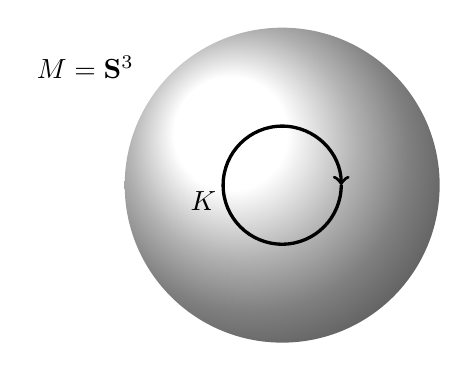
\begin{tikzpicture}
     \shade [ball color=white] (-2,-2.5) circle [radius=2cm];
     \draw (-4.5, -1.0) node {$M = \mathbf{S}^3$};  % label for the sphere, just specify position and done
     \draw [very thick] (-2.75, -2.5) arc (180:360:0.75); % these next 2 lines are for the circle, bottom half first and then top half
     \draw [->,very thick] (-2.75, -2.5) arc (180:0:0.75);
     \draw (-3.0, -2.7) node {$K$};
  \end{tikzpicture}
\quad \quad \quad \, 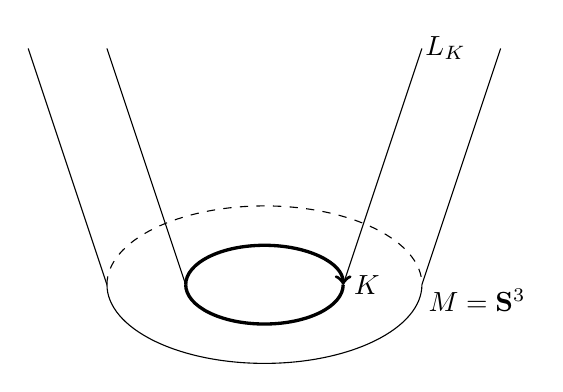
\begin{tikzpicture}
%    \draw (-1,0) arc (180:360:1cm and 0.5cm);  % this is the top
%    \draw (-1,0) arc (180:0:1cm and 0.5cm);
    \draw (-2,-3) arc (180:360:2cm and 1cm);  % these next 2 lines are the bottom circle, with the bottom half first, and then the dashed top half
    \draw[dashed] (-2,-3) arc (180:0:2cm and 1cm);
%    \draw[dashed] (-2,-3) arc (180:10:2cm and 1cm);
%    \draw(-2,-2.9)  -- (-1,0);   % these are ``diagonal lines'' move up and outwards
%    \draw(2,-2.9)   -- (1,0);
\draw [very thick] (-1,-3) arc (180:360:1cm and 0.5cm); % these next 2 lines are for the circle or unknot, first bottom half then top half
\draw [->,very thick] (-1,-3) arc (180:0:1cm and 0.5cm);
\draw(-1,-3.0) -- (-2,0);  % these next 2 lines are the ``inside'' ``diagonal lines'' moving up and outwards into the branes
\draw(1,-3.0) -- (2,0);
\draw(-2,-3.0) -- (-3,0);  % these next 2 lines are the ``outside'' ``diagonal lines'' moving up and outwards into the branes
\draw(2,-3.0) -- (3,0);
\draw (2.7, -3.2 ) node {$M = \mathbf{S}^3$}; % the following are labels; just specify a node (``position'') and place
\draw (1.3, -3) node {$K$};
\draw (2.3,0) node {$L_K$};
\end{tikzpicture}
\end{center}
\caption{For $M$ a 3-manifold, $L_K$ a Lagrangian submanifold, $L_K \bigcap M = K$} \label{Fig:topstringsetup00}
\end{figure}

Let us try to make sense of this setup.  

The topological string on a Calabi-Yau manifold $X$ counts holomorphic maps from Riemann surfaces, $\Sigma$ into target space $X$, i.e. for holomorphic map $\phi : \Sigma \to X$, with $\overline{\partial} \phi =0$ (holomorphic).    Topological sigma models called $A$ model and $B$ model govern these maps from $\Sigma$ to a target space $X$. The $A$ model is concerned with almost holomorphic maps from $\Sigma$ to $X$, while the $B$ model is related to periods of differential forms on $X$.   Let us take the target space to be a Calabi-Yau manifold $X$ that is a 3-fold, i.e. $X$ has 3 complex dimensions.

It was explained that for any three-manifold $M$, the open topological string $\mathbf{A}$ model on $X = T^*M$ with $N$ topological D-branes on $M$ is the same as $SU(N)$ Chern-Simons theory on $M$ \cite{Witten1992}.  The reduction of the $A$ model to Chern-Simons theory is exact, in that since the $A$ model taken is independent of coupling parameter $t$, and as $t$ and target space metric $g_{ij}$ appear only in the combination $tg_{ij}$, the large $t$ limit was taken and shown to reduce the $A$ model action to the ordinary Chern-Simons Lagrangian.  So now contact with knot theory via the Chern-Simons Lagrangian to the open topological string on $X = T^*M$ has been made.

Thus the open topological string in this $A$ model is the same as $SU(N)$ Chern-Simons theory on $M$:
\begin{equation}
Z^{\text{CS}}_{ SU(N) }(M,K;q) = Z^{\text{open}}_{\text{top}  }{ (T^*M, L_K;q) }  \label{eq:CSSUN=opentop}
\end{equation}

%Note simply that the partition function for open topological strings count 

Indeed the string coupling and the level of Chern-Simons, $k$, are related through the topological string coupling $g_s$ by 
\[
g_s = \frac{2\pi i}{ k + N}
\]
and 
\begin{equation}
  q = e^{ \frac{ 2 \pi i }{ k + N} } = e^{g_s} \label{Eq:AmodelCSqgenus}
\end{equation}
The parameter $q$ of Chern-Simons theory is related to the genus in topological string in this manner by \ref{Eq:AmodelCSqgenus}.  

So in the setup in \eqref{Eq:M5theorysetup00}, at least for the top line with spacetime $\mathbb{R} \times T^*M \times M_4$, $SU(N)$ Chern-Simons theory is realized as a open topological string A-model.  

Consider $M = \mathbf{S}^3$ (or, the closely related case of $M = \mathbb{R}^3$) and so the setup (\ref{Eq:M5theorysetup01}) becomes the following: 

\begin{equation}
  \begin{aligned}
    \text{ spacetime }  & \mathbb{R} \times T^*S^3 \times M_4 \\ 
    N \, M5 \text{ brane } & \mathbb{R} \times S^3 \times D \\ 
     \, M5 \text{ brane } & \mathbb{R} \times L_K \times D
\end{aligned} \label{Eq:M5theorysetup01}
\end{equation}

$L_K$ is once again the conormal bundle to $K \subset S^3$ in the Calabi-Yau space $T^*S^3$.  Take $D\cong \mathbb{R}^2$, and $M_4 \cong \mathbb{R}^4$.  $D$ is a surface of $M_4$, i.e. $D\subset M_4$.  This should be okay as long as there is a $U(1)_F \times U(1)_P$ symmetry action, where $U(1)_F$ is a rotation symmetry of the normal bundle of $D\subset M_4$ and $U(1)_P$ is a rotation symmetry of the tangent bundle of $D\subset M_4$ \cite{FujiGukovSulkowski2012}.  The corresponding quantum numbers (conserved charges!) are denoted by $F$, $P$ for $U(1)_F$, $U(1)_P$ rotation symmetries, respectively.  

In turns out that the quantum $q$-grading and the homological $t$-grading are the fugacities (i.e. $q^P$ and $t^F$, respectively) for the equivalent action of $U(1)_P \times U(1)_F$
\begin{equation}
\begin{aligned}
  & z_1 \to qz_1 \\
  & z_2 \to tz_2
\end{aligned}
\end{equation}
where $(z_1, z_2)$ are the local coordinates of $M_4$.  

Note that the first $\mathbb{R}$ for the above setups, (\ref{Eq:M5theorysetup00}) and (\ref{Eq:M5theorysetup01}), is for time.  By time translation symmetry, one can ask for a space of BPS states on multiple $N$ M5-branes in \eqref{Eq:M5theorysetup01} or on a single M5-brane, without the $N$ copies of M5-branes \cite{GukovStosic2012}.  


 % and due to time translation invariance, 


%Step back and consider that for the closed topological string, to obtain a refined index, one counts the BPS states so to obtain a partition function of the theory.   When M-theory on Calabi-Yau $X$ has an extra $U(1)_R$ symmetry, one obtains a new index, the M-theory partition function on $(X\times \mathbb{C}^2 \times S^1)_{q,t}$ where the 

%This can be extended to refine open topological string, corresponding in M-theory to adding M5 branes on the Lagrangian $L_K$ in $X=T^*M$.    


Now in the case of the open topological string, refinement corresponds in M-theory to adding a M5 brane on the Lagrangian submanifold $L_K$ in $X=T^*M$.  In the setup \eqref{Eq:M5theorysetup00} and \eqref{Eq:M5theorysetup01}, there is the M5 brane on $\mathbb{R} \times L_K \times D$.  

Also in this case of the open topological string, there is the insertion of $N$ M5 branes in the M-theory.  

Step back and consider that one counts BPS states so to obtain a partition function.  When M-theory on the Calabi-Yau $X= T^*M$ has an extra $U(1)_R$ symmetry, one obtains a new index for the partition function, the M-theory partition function on $(X \times \mathbb{C}^2 \times S^1)_{q,t}$ where the subscript denotes that as one goes around the $S^1$, the two $\mathbb{C}$ planes get rotated by $(z_1, z_2 ) \to (qz_1, t^{-1}z_2)$, accompanied by the extra $U(1)_R$ symmetry rotation needed to preserve supersymmetry.

When the knot is a torus knot, i.e. $K=T^{m,n}$, it was pointed out \cite{AganagicShakirov2012} that the $M5$-brane theory has this extra $R$-symmetry, $U(1)_R$ acting on $S^3$, leaving the knot $K=T^{m,n}$ invariant and the Lagrangian $L_K \subset T^*S^3$ invariant.  The partition function is supersymmetric.  It should be commented that one can formally construct a knot homology, with grading and categorification, but the partition function with $U(1)_R$ symmetry preserves supersymmetry.  Denote this quantum for $U(1)_R$ $R$-symmetry by $S_R$.  

Introduce the partition function in the particular case of the torus knot so that $K = T^{m,n}$, counting states in the space of BPS states in this refined setup, $\mathcal{H}^{\text{ref}}_{\text{BPS}}$:
\begin{equation}
Z^{\text{ref}}_{\text{BPS}}(S^3, T^{m,n}_R;q,t)  \equiv \text{Tr}_{\mathcal{H}^{\text{ref}}_{\text{BPS}}   }{  (-1)^{S_R} q^{P} t^{F-S_R} }
\end{equation}
which ``counts'' the refined BPS states.  Keep in mind that it was argued in \cite{AganagicShakirov2012} that for some torus knots, all refined BPS states have $S_R =0$.

%For $\text{sl}{(N)}$ knot homology, the partition function is 
%\begin{equation}
%  \mathcal{P}^{ \text{sl}{ (N)}, R  }{ (K, q,t) } = \text{Tr}_{ \mathcal{H}^{\text{ref}}_{ \text{BPS} }  }{  q^P t^F }
%\end{equation}
% and so expressions for $\mathcal{P}^{ \text{sl}{ (N)}, R }{ (K;q,t)}$ and  $Z^{\text{ref}}_{SU(N)}$ agree.  

Note that the large $N$ transition had been studied in \cite{bib:OV2000}. In this dual description, for large $N$, after the geometric transition, the setup now is the following:
\begin{equation}
  \begin{aligned}
 \text{ spacetime }  & \mathbb{R} \times X \times M_4 \\ 
\text{ M5 brane }    & \mathbb{R} \times L_K \times D
\end{aligned}
\end{equation}
where $X$ is the total space of $\mathcal{O}{(-1)} \oplus \mathcal{O}{ (-1)}$ bundle over $\mathbb{C}P^1$.  BPS states carry a new quantum number which becomes an $a$-grading of for the space of BPS states in this refined case (but now in the geometric transition) $\mathcal{H}^{\text{ref}}_{\text{BPS}}$.  The $a$-grading now is exponentiated by the ``winding number'' $\beta \in H_2(X,L_K) \cong \mathbb{Z}$ in the partition function.  

\begin{equation}
  Z^{\text{ref}}_{\text{BPS}}{ (S^3, T^{m,n}_R;a,q,t) } = \text{Tr}_{\mathcal{H}^{\text{ref}}_{ \text{BPS}} }{  (-1)^{ S_R} a^{\beta} q^{P} t^{ F- S_R } }
\end{equation}
This partition function ``counts'' refined BPS states in this geometric transition.  

The noncompact Calabi-Yau 3-fold $X$ deserves some explanation.  $X$ is independent of the knot $K$.  It is defined as the total space of the $\mathcal{O}{ (-1) } \oplus \mathcal{O}{ (-1)}$ bundle over $\mathbb{C}\mathbf{P}^1$.  What is $\mathcal{O}{(-1)}$?  Recall that  a conifold singularity in $\mathbb{C}^4$ for a threefold can be defined with local (complex) coordinates $(X,Y,U,V) \in \mathbb{C}^4$ by the following statement
\[
XY - UV =0 
\]
There is a singularity at $0\in \mathbb{C}^4$.  To \emph{resolve} the singular point, consider the space $Z \subset \mathbb{C}^4 \times \mathbb{P}^1$, defined by 
\[
\left( \begin{matrix} X & U \\
  V & Y \end{matrix} \right) \left( \begin{matrix} 
  \lambda_1 \\
  \lambda_2 \end{matrix} \right) = 0
\]
with $\left( \begin{matrix} \lambda_1 \\ \lambda_2 \end{matrix} \right) \in \mathbb{C}P^1$.  

It can be shown that $Z$ and the conifold is isomorphic outside of the singularity.  

$\mathcal{O}{ (-1)}$ is the fiber for the line bundle constructed from $\mathbb{P}^n$, denoted as such because the dual of the line bundle has inverse transition functions.  It can be shown explicitly that $Z$ is the total space of $\mathcal{O}{ (-1)} \oplus \mathcal{O}{ (-1)}$.  With $Z$, the singular point at $0$ is replaced by $\pi^{-1}{ (0)} = \mathbb{P}^1 \cong S^2$.  Also, there is an extra element in the homology class $H_2$.  By Poincar\'{e} duality, new classes in $h^{2,2}$, $h^{1,1}$ (cohomology) are obtained.  Thus, we have a basic ``local'' (noncompact) Calabi-Yau threefold that resolves the singularity \cite{Hori2003}.

The $a$-grading is the K\"{a}hler parameter of $\mathbb{C}P^1$.  The $a$-deformation has as its interpretation as being one of the K\"{a}hler moduli of this underlying Calabi-Yau geometry $X$.

%Taubes had proposed a systematic construction of the Lagrangian submanifold $\mathcal{L}_K$ from a braid diagram of $K$ \cite{Taubes2001}.  First, a two-dimensional noncompact Lagrangian submanifold $\mathcal{L}_K^{(2)} \subset \mathbb{C}^2$ is constructed, such that $\mathcal{L}_K^{(2)} \bigcap \mathbf{S}^3$ is isotopic to the knot $K$, as displayed in Figure (\ref{Fig:topstringsetup00}).  Then, identify $\mathbf{C}^2 \otimes \mathcal{O}{ (-1)}$ with a fiber of $X$ and define $\mathcal{L}_K$ to be a particular subbundle $\mathcal{L}_K^{(2)} \to \mathbf{S}^1$ of $\mathcal{O}{ (-1) } \oplus \mathcal{O}{ (-1) } \to \mathbb{C}\mathbf{P}^1$ restricted to the equator $\mathbf{S}^1 \subset \mathbb{C}\mathbf{P}^1$ \cite{DunfieldGukovRasmussen2005}.  

Now, it was conjectured that for $sl{(N)}$ knot homology, in order to obtain the knot homology, one simply needs to consider the space of BPS states on an open topological string, namely to consider the space of BPS states of M2-branes \cite{GukovSchwarzVafa2005}.  It would follow that for this refined BPS states counting, we would obtain the triply-graded homology theory for the colored superpolynomials.  

So the partition function for refined BPS states counting, $Z^{\text{open}}_{ \text{BPS}}$, when $S_R=0$,  coincides with colored superpolynomial, in the case of the knot $K$ being a torus knot, $T^{m,n}$:  

\begin{equation}
\begin{aligned}
   Z^{ \text{open}}_{\text{BPS}}{ (T^*S^3, T^{ m,n }_R ; a,q,t) }    & = \text{Tr}_{ \mathcal{H}^{ \text{ref}}_{ \text{BPS}}  }{ a^{ \beta} q^P t^F } =  \\
 &  = \mathcal{P}^R{ (T^{m,n};a,q,t) }
\end{aligned}
\end{equation}

%  Z^{ \text{ref}}{ (S^3, T^{ m,n }_R ; a,q,t) }

Furthermore, remember that from \eqref{eq:CSSUN=opentop}, there was an exact relationship between open topological strings in the A-model and $SU(N)$ Chern-Simons theory.  One would expect that after refinement, this relationships should carry on.  Hence, calling this partition function for the refined Chern-Simons theory with gauge group $SU(N)$, $Z^{\text{ref}}_{SU(N)}{(M,K)}$, 
\begin{equation}
  Z^{\text{ref}}_{SU(N)}{(M, T^{(m,n)}) } = Z^{\text{open}}_{\text{BPS}}{ (T^*M, T^{m,n}_R;a,q,t)}
\end{equation}

To conclude, the colored superpolynomials in the context of knot homologies was introduced in \cite{GukovStosic2012}:
\begin{equation}
\mathcal{P}_r{ (K;a,q,t) } := \sum_{ i,j,k} a^i q^j t^k \text{dim}{ \mathcal{H}_{i,j,k}^{ S^{r} }{ (K) } }
\end{equation}
as a Poincar\'e polynomial of a triply-graded homology theory categorifying the $S^r$-colored HOMFLY-PT polynomial.  In the context of BPS states, $\mathcal{P}_r{(a,q,t)}$ is defined as the generating function of refined open BPS invariants (counting BPS states) on a Calabi-Yau 3-fold $X$, in the presence of the Lagrangian submanifold $L_K \subset X$, and is given by the following:
\begin{equation}
  \mathcal{P}_r{(a,q,t)} \equiv \text{Tr}_{\mathcal{H}^{\text{ref}}_{\text{BPS}} }{ a^{\beta} q^P t^F } \, , \quad \, \beta \in H_2{(X,L_K)}
\end{equation}
The conjecture in \cite{GukovSchwarzVafa2005} says that these two definitions of $\mathcal{P}_r{(a,q,t)}$ give the same result when $X$ is the total space of $\mathcal{O}{(-1)} \oplus \mathcal{O}{(-1)}$ bundle over $\mathbb{C}P^1$ and the Lagrangian submanifold is determined by the knot $K\subset \mathbf{S}^3$, cf. \cite{Taubes2001}, \cite{bib:OV2000}.  

Thus, this $\mathcal{P}_r{ (K;a,q,t)}$ can also be calculated from the viewpoint of the refined Chern-Simons theory and open topological strings.




\section{Cutting and gluing}

To solve a topological field theory on any 3-manifold $M$, with boundary $\Sigma = \partial M$, and with arbitrary knots inside, one needs the $S$ and $T$ matrices, representing the action of $SL(2,\mathbb{Z})$ on the Hilbert space of the theory on $T^2$, and the braiding matrix $\mathcal{B}$ acting on the Hilbert space of the four-punctured sphere.  $S$ and $T$ matrices of a 3-dimensional TQFT are the unitary representation of the action of the modular group $SL{(2,\mathbb{Z})}$ such that 
\begin{equation}
  \begin{aligned}
    & S^4 =1 \\
    & (ST)^3 = S^2
\end{aligned}
\end{equation}
on the Hilbert space $\mathcal{H}_{\Sigma}$.  

In Chern-Simons theory with gauge group $G$, we seek to compute the partition function
\begin{equation}
  Z_G^{\text{CS}} \equiv \int dA \, W_R{ (K)}[A] \exp{ \left( ik S_{\text{CS}}{ [A;M] } \right) }
\end{equation}
%the necessary ingredients include the $S$ and $T$ matrices and a braiding operator $\mathcal{B}$.  



Let $K_R$ be a knot in the 3-manifold $M$, colored by the fundamental representation $R$ of the gauge group $G=SU(N)$ (in this case).  Consider dividing the 3-manifold $M$ into two pieces $M_1$ and $M_2$ along a surface $\Sigma$.  As with axiomatic TQFT, $|\psi_{M_1;K_R} \rangle$ and $|\psi_{M_2;K_R}\rangle$ are elements of $\mathcal{H}_{\Sigma}$.  The partition function $Z^{\text{CS}}_{ SU(N)}{ (M;K_R;q)}$ is the pairing or ``inner product'' of these two elements in the physical Hilbert space $\mathcal{H}_{\Sigma}$:
\begin{equation}
Z^{\text{CS}}_{ \text{SU}{(N)} }(M, K_R;q) = \langle \psi_{M_2;K_R} | \psi_{M_1;K_R} \rangle
\end{equation}

The physical Hilbert space $\mathcal{H}_{\Sigma}$ is the space of conformal blocks obtained by canonical quantization of the Chern-Simons gauge theory\cite{Witten1989}:

\[
\mathcal{H}_{\Sigma} \simeq \lbrace \text{ conformal blocks for $G/G$ WZW model on $\Sigma$ } \rbrace
\]
where $G = SU(N)$.  If the knot $K_R$ meets the surface $\Sigma$ at $m$ points, the physical Hilbert space $\mathcal{H}_{\Sigma; R_1 \dots R_m}$ consists of conformal blocks of $m$-point functions with carry representations $R_a = R$ or $\overline{R}$ $(a=1, \dots , m)$, depending on the orientation at the intersection.  

For the torus knots $T^{2,2p+1}$ in a 3-sphere $\mathbf{S}^3$, consider slicing $\mathbf{S}^3$ into a pair of 3-dimensional balls $\mathbf{B}^3$ connected by a cylinder.  The physical Hilbert space $\mathcal{H}_{ \mathbf{S^2}; R R \overline{R} \overline{R} }$ for this slice consists of conformal blocks for the four-point function:

\begin{equation}
  \phi_Q{ (R,R, \overline{R}, \overline{R})}, \quad \, Q \in R\otimes R
\end{equation}
where $Q$ is the irreducible representation $Q \in R\otimes R$.  In general, $\mathcal{H}_{\mathbf{S}^2; R_1R_2R_3R_4}$ is spanned by the orthonormal states

\begin{equation}
  \langle \phi_{Q'}{ (R_1, R_2, R_3, R_4) } | \phi_Q{ (R_1, R_2, R_3, R_4)} \rangle = \delta_{QQ'}, \quad \, Q,Q' \in R_1 \otimes R_2
\end{equation}

Thus, for the state $|\psi_0(R_1,R_2)\rangle \in \mathcal{H}_{\mathbf{S}^2; R_1R_2 \overline{R}_2 \overline{R}_1}$, consider the following expansion:

\begin{equation}
  |\psi_0{ (R_1,R_2) } \rangle = \sum_{Q \in R_1 \otimes R_2} \mu^Q_{R_1R_2} | \phi_Q{ (R_1, R_2, \overline{R}_2,\overline{R}_1 ) }\rangle
\end{equation}

The coefficient $\mu^Q_{R_1R_2}$ can be obtained by pairing this state (taking the ``inner product'') with itself:

\begin{equation}
\begin{aligned}
  \langle \psi_0{(R_1,R_2)} |\psi_0{ (R_1,R_2)}\rangle & = \sum_{ Q \in R_1\otimes R_2} \left( \mu^Q_{R_1R_2} \right)^2 = \\
  & = Z^{\text{CS}}_{ \text{SU}{(N)} }{ ( \mathbf{S}^3, \circlearrowleft_{R_1} \circlearrowleft_{R_2}; q)}
\end{aligned}
\end{equation}

Since the two unknots are not linked, by the associativity property for a TQFT (or by slicing along another surface $\Sigma_2 \cong \mathbf{S}^2$), then we have the following:

\begin{equation}
  Z^{ \text{CS}}_{ \text{SU}{(N)}}{ (\mathbf{S}^3, \circlearrowleft_{R_1} \circlearrowleft_{R_2};q ) } Z^{ \text{CS}}_{ \text{SU}{ (N)} }{ (\mathbf{S^3};q) } = Z^{\text{CS}}_{ \text{SU}{(N)} }{ ( \mathbf{S}^3, \circlearrowleft_{R_1}; q) } Z^{\text{CS}}_{ \text{SU}{ (N)}}{ (\mathbf{S}^3, \circlearrowleft_{R_2};q)}
\end{equation}

The partition function of the unknot $\circlearrowleft_R$ in $\mathbf{S}^3$ is given by the quantum dimension:

\begin{equation}
  \frac{ Z^{\text{CS}}_{ \text{SU}{ (N) }}{ ( \mathbf{S}^3, \circlearrowleft_R;q) } }{ Z^{ \text{CS}}_{ \text{SU}{(N)} }{ (\mathbf{S}^3;q) } } = \text{dim}_q{ R}
\end{equation}

The quantum dimension $\text{dim}_q{R}$ is a specialization of the Schur polynomial $s_R{(x)}$:

\begin{equation}
\text{dim}_q{R} = s_R{ (q^{ \varrho} ) }, \quad \, \varrho = (\varrho_1, \dots , \varrho_N), \quad \, \varrho_i = \frac{N+1}{2} -i  
\end{equation}

The Schur polynomial $s_R{(x)}$ obey the following identity:

\begin{equation}
  s_{R_1}{ (x)} s_{R_2}{ (x)} = \sum_{ Q \in R_1 \otimes R_2} s_Q{(x)}
\end{equation}

Using the above results, the coefficient $\mu_Q$ is determined as 

\begin{equation}
  \left( \mu^Q_{R_1R_2} \right)^2 = s_Q{ (q^{ \varrho} ) } Z^{\text{CS}}_{ \text{SU}{(N)}}{ (\mathbf{S}^3; q)}
\end{equation}

The state $|\psi_{2p+1}{ (R_1, R_2) } \rangle$ is constructed by acting $2p+1$ times with a braid operator $\mathcal{B}_{R_1 R_2}$ on the 3-ball state $|\psi_0{(R_1,R_2)} \rangle$:

\begin{equation}
  | \psi_{2p+1}{ (R_1 , R_2) } \rangle = \mathcal{B}^{2p+1}_{ R_1 R_2} | \psi_0{ (R_1,R_2)} \rangle
\end{equation}

The action of the braid operator $\mathcal{B}_{R_1R_2}$ on the conformal block $\phi_Q{ (R_1, R_2,R_3,R_4)}$ obeys a monodromy transformation (copies of $R_a$ and $R_b$ exchange places by taking half-steps, revolving around each other).  The eigenvalue of the monodromy for the conformal block, $\lambda^{(+)}_Q{ (R_1,R_2)}$ was determined in \cite{MooreSeiberg1989}.  

Thus, $Z^{\text{CS}}_{\text{SU}{(N)}  }{ (\mathbf{S}^3, T_R^{2,2p+1}; q) }$ can be evaluated from the braid operator $\mathcal{B}^{2p+1}_{RR}$ as follows:
\begin{equation}
  \begin{aligned}
    Z^{\text{CS}}_{ \text{SU}{(N)} }{ ( \mathbf{S}^3, T_R^{2,2p+1}; q) } & = \langle \psi_0{ (R,R)} | \mathcal{B}_{RR}^{2p+1} | \psi_0{ (R,R) } \rangle  = \\
&    = \sum_{Q\in R\otimes R} \lambda_Q^{ (+)}{ (R,R)}^{2p+1} \left( \mu^Q_{RR} \right)^2 = \\ 
&    = Z^{ \text{CS}}_{ \text{SU}{(N)}}{ (\mathbf{S}^3; q) } \sum_{Q \in R\otimes R} \lambda_Q^{(+)}{ (R,R)}^{2p+1} \text{dim}_qQ
  \end{aligned}
\end{equation}


\section{Colored superpolynomial from Refined Chern-Simons theory}

%It was assumed that the generating functions of the refined BPS invariants could be expressed in the form of a amplitude with a Hilbert space whose states are labeled by conformal blocks \cite{FujiGukovSulkowski2012}.  

Refined versions of the $S$ and $T$ modular matrices were proposed in \cite{AganagicShakirov2012} and were adopted in computing the colored superpolynomials for the torus knots.  The refinement in the quadratic Casimir factor $q^{C_2{(R)}}$, which is related to the $T$ modular matrices,
\begin{equation}
  q^{C_2{(R)}} \leadsto q_1^{ \frac{1}{2} \| R\|^2} q_2^{ -\frac{1}{2} \| R^T\|^2} q_2^{ \frac{N}{2} |R| } q_1^{-\frac{1}{2N} |R|^2 }
\end{equation}
was used to for the refinement of the eigenvalues for the braid operator, $\lambda^{(+)}_Q{(R,R)}^{2p+1}$.  Note that $R^T$ denotes the transposition of the Young diagram of the representation $R$.  

Let the power sum symmetric function in $x = (x_1, x_2, \dots)$ be defined as $p_n \equiv \sum_{i=1}^{\infty} x_i^n$.  The MacDonald polynomials $M_R(x;q_1,q_2)$ are $q_1,q_2$ generalizations of the Schur functions and monomial symmetric functions.  The existence of the Macdonald polynomial for an affine root system can be shown \cite{Warnaar}.  Nevertheless, in the case at hand, representation $R$ is the totally symmetric or totally antisymmetric representation.

Instead of Schur functions for the partition function of the unknot, the refined analogue for the refined partition function of the unknot is now the following, involving MacDonald polynomials:
\begin{equation}
  \frac{ Z^{ \text{ref} }_{SU(N)}(\mathbf{S}^3, \circlearrowleft_R; q_1, q_2) }{ Z^{ \text{ref} }_{SU(N)}{ (\mathbf{S}^3; q_1, q_2 ) } } = M_R{ (q_2^{ \varrho}; q_1,q_2) }
\end{equation}
where the MacDonald polynomial is the following:
\begin{equation}
  M_R{ (q_2^{\varrho}; q_1, q_2) } = \prod_{ (i,j) \in R }  \frac{q_2^{  \frac{ N- i + 1}{2} } q_1^{ \frac{j-1}{2} } - q_2^{ - \frac{N-i + 1}{2} } q_1^{ - \frac{j-1}{2} } }{  q_2^{ \frac{R_j^T - i + 1 }{2} } q_1^{ \frac{R_i - j}{2} } - q_2^{ - \frac{ R_j^T - i + 1 }{2} } q_1^{ - \frac{R_i - j }{2} } }
\end{equation}

The Macdonald polynomial satisfies an identity that is an analogue to the identity that the Schur functions obey:
\begin{equation}
M_{R_1}{ (x;q_1, q_2) }M_{R_2}{ (x;q_1,q_2) } = \sum_{ Q \in R_1 \otimes R_2 }N^Q_{R_1R_2}M_Q{ (x;q_1,q_2) }
\end{equation}
where $N_{R_1R_2}^Q$ is a rational function of $q_1,q_2$, namely the Littlewood-Richardson coefficients.  

The partition function $Z^{\text{ref}}_{SU(N)}{ ( \mathbf{S}^3, T_R^{2,2p+1};q_1,q_2) }$ for the $T^{2,2p+1}$ torus knot is once again in the form of an amplitude with Hilbert spaces sandwiching the braid operator $(\mathcal{B}^{2p+1})_{RR}$:
\begin{equation}
\begin{gathered}
  Z^{\text{ref}}_{SU{(N)} }{ ( \mathbf{S}^3, T_R^{2,2p+1};q_1,q_2)  } = \langle \psi_0(R,R) | (\mathcal{B}^{2p+1})_{RR} | \psi_0(R,R) \rangle =    \\
    = Z^{\text{ref}}_{ SU{(N)} }{ (\mathbf{S}^3;q_1,q_2) } \sum_{ Q \in R\otimes R} \gamma^Q_{RR} \cdot \lambda_Q^{ (+)}{ (R,R)}^{2p+1} \cdot N^Q_{RR} \cdot M_Q{ (q^{\varrho}_2;q_1,q_2)}  
\end{gathered}  \label{eq:ZrefTorus00}
\end{equation}
where gamma factors $\gamma^Q_{RR}$ were introduced.  The gamma factors are needed to make the partition function for the torus knot invariant under the symmetry $T^{n,m} \leftrightarrow T^{m,n}$:
\begin{equation}
Z^{\text{ref}}_{ SU{(N)} }{ (\mathbf{S}^3, T^{n,m}_R;q_1,q_2) } = Z^{\text{ref}}_{  SU{(N)} }{ (\mathbf{S}^3, T^{m,n}_R; q_1,q_2) }
\end{equation}

The gamma factors were determined \cite{FujiGukovSulkowski2012} by using an explicit form for the Littlewood-Richardson coefficients $N^Q_{RR}$ for the symmetric representation $R=S^r$ and antisymmetric representation $R= \Lambda^r$.  The Littlewood-Richardson coefficients were derived from the Pieri formula for $R=S^r$, and $R=\Lambda^r$.   Then, simply a single consistency condition needs to be done for the case of $p=0$, i.e. for $T^{2,1} \cong \circlearrowleft$, to reobtain the unknot.  Thus the gamma functions are determined.

With the symmetric representations $R=S^r$, make the following change of variables
\begin{equation}
  \begin{aligned}
    & a = A \left( \frac{q_1}{q_2} \right)^{3/2} \\ 
    & q = \frac{1}{q_2 } \\
    & t = - \sqrt{ \frac{q_2}{q_1 } }
\end{aligned}
\end{equation}
and write the refined partition functions in terms of $a,q,t$.  


The unreduced superpolynomial $\overline{\mathcal{P}}^{ S^r}( \circlearrowleft; a,q,t)$ of the unknot is now the following:

\begin{equation}
\begin{aligned}
  \overline{ \mathcal{P}}^{S^r} & = \frac{ Z^{\text{ref}}_{SU(N)}{ (\mathbf{S}^3, \circlearrowleft_{\Lambda^r}; q_1,q_2) } }{  Z^{\text{ref}}_{SU(N)}{ (\mathbf{S}^3;q_1,q_2) } } = M_{\Lambda^r}{ (q_2^{\varrho}; q_1, q_2 ) } = \\
  & = (-1)^r A^{r/2} q_2^{r/2}  \frac{ (A^{-1}; q_2 )_r }{ (q_2;q_2)_r } = (-1)^{ \frac{r}{2} } a^{ -\frac{r}{2} } q^{ \frac{r}{2} } t^{ - \frac{3r}{2} } \frac{ (-at^3;q)_r }{ (q;q)_r } 
\end{aligned} \label{Eq:unreducedPaqtUnknotrefinedCS}
\end{equation}

Similarly, the reduced colored superpolynomial of the general $(2,2p+1)$ torus knot is related to the partition function $Z^{\text{ref}}_{SU(N)}{ (\mathbf{S}^3, T^{2, 2p+1 }_{\Lambda^r};q_1,q_2) }$ by a refined analogue to \eqref{Eq:CStheoryJonespolynomial00}:

\begin{equation}
  \mathcal{P}^{S^r}(T^{ 2, 2p+1}; a,q,t) = \left( \frac{q_1}{q_2} \right)^{  \frac{pr}{2} } \frac{ Z^{\text{ref}}_{SU(N)}{ (\mathbf{S}^3, T^{2, 2p+1}_{\Lambda^r}; q_1,q_2 ) } }{ Z^{\text{ref}}_{SU(N)}(\mathbf{S}^3, \circlearrowleft_{\Lambda^r};q_1,q_2) }
\end{equation}

With \eqref{eq:ZrefTorus00}, along with the gamma factors, refined braid operator eigenvalues, Littlewood-Richardson coefficients, and MacDonald polynomials, the form of the colored superpolynomial is the following:
\begin{equation}
\begin{gathered}
  \mathcal{P}^{S^r}( T^{(2,2p+1)}; a,q,t ) = \sum_{ l=0}^r \frac{ (qt^2; q)_l (-at^3; q)_{r+l} (-aq^{-1} t; q)_{r-l} (q;q)_r }{ (q,q)_l (q^2 t^2; q)_{r+l} (q;q)_{r-l} (-at^3; q)_r } \frac{ ( 1 - q^{2l + 1} t^2 ) }{ (1-qt^2 ) } \cdot \\
  \cdot (-1)^r a^{ - \frac{r}{2} } q^{ \frac{3r}{2} - l } t^{ -rp - l + \frac{r}{2} } \left[ (-1)^l a^{\frac{r}{2} } q^{  \frac{r^2 - l (l+1  ) }{ 2}  }t^{ \frac{3r}{2} - l } \right]^{2p+1}
\end{gathered}
\end{equation}

Now simply recall the following identity for the $q$-binomial:

\[
\frac{ (q;q)_r }{ (q;q)_l (q;q)_{r-l } } = { r \brack l } 
\]

Then

\begin{equation}
\begin{gathered}
\mathcal{P}^{ S^r}(T^{(2,2p+1) }; a,q,t )= \sum_{l=0}^r \frac{ (qt^2 ; q)_l (-at^3; q)_{r+l} ( -aq^{-1} t; q)_{r-l } }{ (q^2 t^2 ; q)_{r+l } (-at^3 ; q)_r } { r \brack l } \frac{ ( 1-q^{2l + 1 } t^2 ) }{ ( 1- qt^2 ) } \cdot \\
\cdot (-1)^r a^{-\frac{r}{2} } q^{ \frac{3r}{2} -l } t^{-rp  - l + \frac{r}{2} } \left[ (-1)^l a^{\frac{r}{2} } q^{  \frac{ r^2 - l (l+1 ) }{2} } t^{ \frac{3r}{2} - l } \right]^{2p+1} 
\end{gathered} \label{Eq:coloredsuperpolytorusknotrefinedCS}
\end{equation}
which is the expression used for computation in this work.  

For instance, for the case of the trefoil, $\mathcal{P}^{S^r}{(a,q,t)}$ becomes the following:
\begin{equation}
\mathcal{P}^{S^r}{(T^{(2,3)}; a,q,t)} = a^r q^{-r} \sum_{k=0}^r \frac{ ( q^r, q^{-1} )_k }{ (q,q)_k } q^{(r+1)k } t^{2k} ( -aq^{-1} t; q )_k  \label{Eq:coloredsuperpolytrefoilrefinedCS}
\end{equation}





\chapter{Quantum super-A-polynomials} \label{chap:quantumsuperApolynomials}

In this chapter, the refined Volume Conjectures \cite{FujiGukovSulkowski2012} are first noted as the refinement/categorification of the generalized volume conjecture \cite{Gukov2005}.  Then the new volume conjectures \cite{bib:FGS2012} for the colored superpolynomials, which has played a prominent role during this work, involving their asymptotic behavior relation to the super-A-polynomial and the construction of the quantum super-A-polynomials are presented.  The specializations of the quantum super-A-polynomials and the classical super-A-polynomials into the polynomial and homological invariants of knots reviewed in this work are discussed.  While all the quantum super-A-polynomials that were computed in this work are collected in Appendix \ref{app:qsAp}, examples for the unknot, trefoil, and cinquefoil are discussed.  The specializations of these quantum super-A-polynomials support the volume conjectures made in \cite{bib:FGS2012}, \cite{FujiSulkowski2013}.

\section{Refined and categorified volume conjectures}

Recall from \eqref{eq:eulerJonessl2homo00}, the Poincar\'{e} polynomials $\mathcal{P}_n{(K;q,t)}$ are the categorification of the colored Jones polynomial $J_n{ (K;q)}$

\begin{equation}
\mathcal{P}_n{ (K; q,t) } = \sum_{i,j}q^i t^j \text{dim}{ \mathcal{H}_{i,j}^{ sl{ (2)}, R }{ (K)} }
\end{equation}
such that the Euler characteristics of this Poincar\'{e} polynomial $\mathcal{P}_n{(K;q,t)}$ gives back the colored Jones polynomial:
\begin{equation}
J_n{ (K;q) } = \mathcal{P}_n{ (K; q,t=-1)}
\end{equation}

Fuji, Gukov, and Su\l kowski made the conjectures that generalizes the generalized volume conjecture and its ``quantum'' version, the AJ-conjecture, for the case of this refinement/categorification \cite{FujiGukovSulkowski2012}. Keep in mind that this refinement/categorification involves an extra $t$-parameter, or $t$-deformation, or grading.      

Remember that the generalized volume conjecture was in the context of Chern-Simons with complex gauge group $G_{\mathbb{C}} = SL{(2,\mathbb{C})}$ and involved partition functions with Wilson loops of the Chern-Simons theory with compact gauge group $G=SU(2)$.  But in this refinement/categorication, the partition functions to be considered, $Z^{\text{open}}_{\text{BPS}}$, are in the context of refined open topological string theory on a toric Calabi-Yau manifold, with the toric Calabi-Yau manifold being in the presence of branes \cite{FujiGukovSulkowski2012}.  These partition functions are the generating functions for the refined BPS states.  The computation of these partition functions can be made combinatorially by considering the refined topological vertex \cite{bib:IKV2009}. 

Thus, there is a knot homology way of thinking about this refined/categorified conjecture, involving $\mathcal{P}_n{(K;q,t)}$ and another viewpoint from the refined open topological string theory that will count refined BPS states, $Z^{\text{open}}_{\text{BPS}}$.  

The refinement / categorification of the generalized volume conjecture takes the following limit:
\begin{equation}
  q = e^{\hbar} \to 1, \quad \, t = \text{ fixed }, \quad \, x \equiv e^u = q^n = \text{ fixed }  \label{eq:limitrefinedVC}
\end{equation}
The new $t$-parameter is fixed.  Recall that $x$ is related to the eigenvalue of the representation of the holonomy and $u$ is a complex number.  

In this limit \eqref{eq:limitrefinedVC}, $\mathcal{P}_n{(K;q,t)}$ is conjectured to have this asymptotic behavior  \cite{FujiGukovSulkowski2012}:
\begin{equation}
  \mathcal{P}_n \simeq \exp{ \left( \frac{1}{ \hbar} S_0{ (u,t) } + \sum_{n=0}^{\infty} S_{n+1}{ (u,t) } \hbar^n \right) } \quad \quad \, \text{ knots }  \label{Eq:refinedVolumeConjecture00}
\end{equation}

From the viewpoint of the refined open topological string theory, with the partition function being the generating functions for the refined BPS states, in the limit \eqref{eq:limitrefinedVC}, then the conjecture takes this form\cite{FujiGukovSulkowski2012}:
\begin{equation}
  Z^{\text{open}}_{\text{BPS}}{ (u,q,t)} \simeq \exp{ \left( \frac{1}{ \hbar} S_0{ (u,t)} + \sum_{n=0}^{ \infty} S_{n+1}{ (u,t) } \hbar^n \right) } \quad \quad \, \text{ (BPS states) }
\end{equation}

In both cases, $S_0$ is the leading term, which can be thought of as the ``classical action'' in this asymptotic limit:
\begin{equation}
  S_0{ (u,t)} = \int v du = \int \log{y} \frac{dx}{x}
\end{equation}
with the integral done on the zero locus of the \emph{refined} A-polynomial, an A-polynomial with this new $t$-parameter:
\begin{equation}
  \mathcal{C}^{\text{ref}} : \lbrace (x,y) \in \mathbb{C}^* \times \mathbb{C}^* | A^{\text{ref}}{ (x,y;t) } = 0 \rbrace  \label{eq:refinedA0locus}
\end{equation}


\section{New volume conjectures}

Recall from chapter \ref{chap:Categorification}, that the colored superpolynomials are the Poincar\'{e} polynomials $\mathcal{P}_n{(K;a,q,t)}$ are the categorification of the colored HOMFLY-PT knot polynomials $P_n{(K;a,q)}$
\begin{equation}
  \mathcal{P}_n{(a,q,t)} = \sum_{ijk} a^i q^j t^k \text{dim}{ \mathcal{H}_{ijk}{ (K)} }
\end{equation}
such that the Euler characteristics of this Poincar\'{e} polynomial $\mathcal{P}_n{(K;a,q,t)}$ gives back the colored HOMFLY-PT polynomial:
\begin{equation}
  P_n{(K;a,q)} = \mathcal{P}_n{(K;a,q,t=-1)}
\end{equation}

Fuji, Gukov, and Su\l kowski proposed new volume conjectures involving the colored superpolynomials $\mathcal{P}_n{(K;a,q,t)}$ and its relations to a \emph{super-A-polynomial} \cite{bib:FGS2012}, \cite{FujiSulkowski2013}.  These new volume conjectures are taken in the following limits:
\begin{equation}
  q = e^{\hbar} \to 1, \quad \, a = \text{ fixed}, \quad \, t = \text{ fixed}, \quad \, x = q^n = \text{fixed} \label{Eq:FSVolConj1a}
\end{equation}
Note that in this limit, effectively $n$ becomes large, as $x$ is fixed, and so this limit is the ``large color'' limit.  Note also the new parameter $a$ that is held fixed.  

\begin{conjecture}%  [1]
 In the limit \eqref{Eq:FSVolConj1a},
%the $n$-colored superpolynomials $\mathcal{P}_n(K;a,q,t)$ exhibit the following ``large color'' behavior:
\begin{equation} 
  \mathcal{P}_n(K;a,q,t) \overset{ \mbox{ \scriptsize{  $\begin{gathered} n\to \infty \\ \hbar \to 0 \end{gathered}$ } }  }{ \sim } \exp{ \left( \frac{1}{ \hbar } \int \log{ y } \frac{dx}{ x } + \dots \right) } = \exp{ \frac{1}{\hbar} \widetilde{ \mathcal{ W } } + \dots  } \label{Eq:FSVolConj1b}
\end{equation}
The leading term is given by an integral on the zero locus of the super-A-polynomial, i.e. where 
\begin{equation}
  A^{\text{super}}(x,y;a,t) = 0 \label{Eq:FSVolConj1c}
\end{equation}
$\widetilde{ \mathcal{W} }$ is called the potential given by the following:
\begin{equation}
\widetilde{ \mathcal{W}} = \int \log{y} \frac{dx}{x}   \label{Eq:potentialW00}
\end{equation}
The ellipsis represents the regular terms in $\hbar$ (as $\hbar \to 0$) in \eqref{Eq:FSVolConj1b}
\end{conjecture}

The colored HOMFLY-PT polynomial is in two variables, $a$ and $q$, and so one could think of $a$ as an $a$-deformation, as the colored HOMFLY-PT polynomial reduces to the colored Jones polynomial in certain specializations of $a$.  There is a $t$-deformation for the refined A-polynomial, \eqref{eq:refinedA0locus}.  One would want to combine the two deformations into the super-A-polynomial.  Also, chapter \ref{chap:Quantization}, gives a procedure for quantization of this super-A-polynomial.  One would like to combine the non-commutative $q$-deformation with the two commutative $t$- and $a$-deformations into a quantum operator $\widehat{A}^{\text{super}}(\widehat{x},\widehat{y};a,q,t)$.  This operator $\widehat{A}^{\text{super}}(\widehat{x}, \widehat{y};a,q,t)$ is called the \emph{quantum super-A-polynomial}.  Thus, there is a new quantum volume conjecture \cite{bib:FGS2012}, \cite{FujiSulkowski2013}:
\begin{conjecture} % [2]
  For a given knot $K$, the colored superpolynomial $\mathcal{P}_n(K;a,q,t)$ satisfies the following recursion relation
\begin{equation}
  a_k \mathcal{P}_{n+k}(K; a,q,t) + \dots + a_1 \mathcal{P}_{n+1}(K;a,q,t) + a_0 \mathcal{P}_n(K;a,q,t) = 0  \label{Eq:FSVolConj2a}
\end{equation}
where $\widehat{x}$ and $\widehat{y}$ act on $\mathcal{P}_n(K;a,q,t)$ in the following, non-commutative manner:
\begin{equation}
  \begin{aligned}
    & \widehat{x}\mathcal{P}_n = q^n \mathcal{P}_n = x \mathcal{P}_n \\ 
    & \widehat{y} \mathcal{P}_n = \mathcal{P}_{n+1}
  \end{aligned} \label{eq:xycoloredsP}
\end{equation}

The rational functions $a_i \equiv a_i(\widehat{x},a,q,t)$ are the coefficients of a ``quantum super-A-polynomial'':
\begin{equation}
  \widehat{A}^{\text{super}}(\widehat{x},\widehat{y}; a,q,t) = \sum_i a_i(\widehat{x}, a,q,t)\widehat{y}^i  \label{Eq:FSVolConj2b}
\end{equation}
%The cowhose characteristic polynomial is $A^{\text{super}}(x,y;a,t)$
\end{conjecture}

\eqref{Eq:FSVolConj2b} can be rewritten in the following the compact form or notation:
\begin{equation}
  \widehat{A}^{\text{super}} \mathcal{P}_*(K;a,q,t) = 0
\end{equation}
%Again, note that in the notation for the symmetric group, we will use the notation $S^r$ with $r = n-1$.  Indeed, this $r$ would be the rank of the symmetric group.  

One should take stock that the zero locus of the super-A-polynomial, itself an $a$- and $t$- deformation of the A-polynomial, leads to an algebraic curve (variety) that involves the symplectic form with $x$ and $y$, and it makes a connection, through these new conjectures, to the knot homology of the HOMFLY-PT knot polynomial.  

So by various specializations of the $a$-, $t$-, and $q$-deformations, and in particular the classical limit as $q\to 1$, the quantum super-A-polynomial unifies many polynomial and homological invariants of knots that are present.  For the various quantum operators that arise from quantizing the A-polynomial with various deformations, and thus providing recursion relations for the corresponding knot polynomials and homological invariants in those specific deformations, Figure (\ref{Fig:TableqsAp}) tabulates these quantum operators:
\begin{figure}[h]
\begin{center}
  \begin{tabular}{ l c r }
    \textbf{Quantum operator } & \textbf{ provides recursion for } & \textbf{ classical limit } \\
    \hline
    $\widehat{A}^{\text{super}}{ (\widehat{x}, \widehat{y}; a,q,t) }$ & colored superpolynomial $\mathcal{P}^R{(a,q,t)}$ & $A^{ \text{super}}{ (x,y;a,t)}$ \\
    $\widehat{A}^{\text{ref}}{ (\widehat{x},\widehat{y}; q,t) }$ & colored $sl{ (2)}$ homology & $A^{\text{ref}}{ (x,y;t) }$ \\
    $\widehat{A}^{ \text{Q-def} }{(\widehat{x},\widehat{y}; a,q)}$ & colored HOMFLY-PT polynomial & $A^{\text{Q-def}}{ (x,y;a) }$ \\
    $\widehat{A}{ (\widehat{x}, \widehat{y};q)}$ & \text{ colored Jones polynomial} & $A(x,y)$
\end{tabular}
\caption{Table of quantum super-A-polynomials and their specializations, leading to recursion relations for various $S^n$-colored knot invariants} \label{Fig:TableqsAp}
\end{center}
\end{figure}


\begin{figure}[h]
\begin{center}
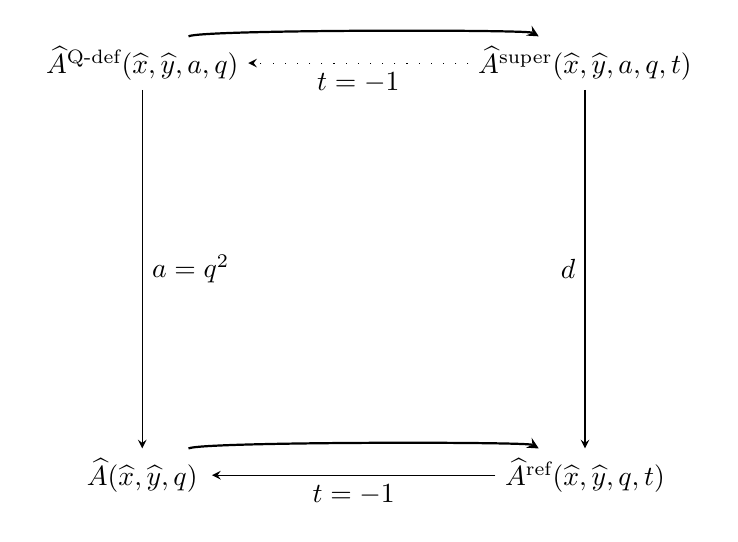
\begin{tikzpicture}
  \matrix (m) [matrix of math nodes, row sep=13em, column sep=8em, minimum width=5em]
  {
    \widehat{A}^{\text{Q-def}}{ (\widehat{x},\widehat{y},a,q) }  &  \widehat{A}^{ \text{super}}{ (\widehat{x},\widehat{y},a,q,t) }  \\
    \widehat{A}{ (\widehat{x},\widehat{y},q)}  &  \widehat{A}^{\text{ref}}{ (\widehat{x},\widehat{y},q,t)}    \\ };
  \path[-stealth]
  (m-1-1) edge[thick,bend left, looseness = 0.1] (m-1-2)
  edge node [auto] {$a=q^2$} (m-2-1)
  (m-1-2) edge[loosely dotted] node [below] {$t=-1$} (m-1-1)
  edge node [left] { $d$} (m-2-2)
  (m-2-1) edge[thick,bend left, looseness = 0.1] (m-2-2)
  (m-2-2) edge node [below] {$t = -1 $} (m-2-1);
\end{tikzpicture} 
\end{center}
\caption{ quantum super-A-polynomials and their specializations.  }
\label{Fig:qsuperApolyspecializations}
\end{figure}

The specializations of the quantum super-A-polynomial are summarized in Figure \ref{Fig:qsuperApolyspecializations}.  What is new are, from Figure \ref{Fig:qsuperApolyspecializations}, from starting from the upper right-hand corner with the quantum super-A-polynomial $\widehat{A}^{\text{super}}{(\widehat{x},\widehat{y};a,q,t)}$, are the specializations to the left with $t=-1$, corresponding to $t=-1$, and down, possibly, to the quantum version of the refined A-polynomial, $\widehat{A}^{\text{ref}}{(\widehat{x},\widehat{y};q,t)}$, which provides a recursion relation for the colored $sl{(2)}$ homology.  

Once again, moving to the left side of Figure \ref{Fig:qsuperApolyspecializations}, where $t=-1$, corresponds to decategorification, and no differentials from the knot homologies are involved with the knot polynomial invariants.  So since the specialization of the colored superpolynomial $\mathcal{P}_n{ (K;a,q,t)}$ to $t=-1$, yields the colored HOMFLY-PT polynomial, as depicted in Figure (\ref{Fig:CatcoloredsuperPoly01}), we should expect that for $t=-1$, the recursion relation as encapsulated by $\widehat{A}^{ \text{super}}{ (\widehat{x}, \widehat{y};a,q,t)}$ should reduce to the recursion relation on the $S^r$-colored HOMFLY-PT polynomials, as encapsulated by the quantum operator denoted by $\widehat{A}^{Q-\text{def}}{ (\widehat{x},\widehat{y};a,q)}$.  
\begin{equation}
    \widehat{A}^{\text{super}}{ ( \widehat{x}, \widehat{y}; a, q,t=-1) } = \widehat{A}^{Q-\text{def}}{ (\widehat{x}, \widehat{y}; a,q)} \label{eq:qsApt=-1}
\end{equation}

In the classical limit case, with the $\mathcal{H}$-thin knots, such as the torus and twist knots, the specialization of $a=q^2$ from the super-A-polynomial $A^{\text{super}}(x,y;a,t)$ yields the refined A-polynomial for the colored $\text{sl}{(2)}$ knot homology.  This has been checked in a number of examples with the torus and twist knots \cite{bib:FGS2012}, \cite{FujiSulkowski2013}, \cite{NRZ2013}.  Furthermore, just as the colored HOMFLY-PT polynomial reproduces the colored Jones polynomial in the specialization of $a=q^2$, then for the left hand side of Figure \ref{Fig:qsuperApolyspecializations}, the specialization of $a=q^2$ for the quantum operator $\widehat{A}^{Q-\text{ref}}$ gives the quantum operator for the A-polynomial, $\widehat{A}{(\widehat{x},\widehat{y};q)}$.  What happens on the right side of Figure \ref{Fig:qsuperApolyspecializations}, starting from the quantum super-A-polynomial, $\widehat{A}^{\text{super}}$?  If $K$ is a thin knot, one would expect that this specialization $a=q^2$ for the quantum super-A-polynomial $\widehat{A}^{\text{super}}{(\widehat{x},\widehat{y};a,q,t)}$ would reduce to a quantized refined A-polynomial, $\widehat{A}^{\text{ref}}{(\widehat{x}, \widehat{y};q,t)}$ that gives a recursion relation for the colored $sl{(2)}$ homology and reproduces the refined volume conjectures \cite{FujiGukovSulkowski2012}, in Eq. \eqref{Eq:refinedVolumeConjecture00}.  In other words, what is expected is the following  \cite{bib:FGS2012}, \cite{FujiSulkowski2013}:

\begin{equation}
  \widehat{A}^{\text{super}}{ ( \widehat{x}, \widehat{y}; a=q^2, q,t) } = \widehat{A}^{\text{ref}}{ (\widehat{x}, \widehat{y}; q,t)} \label{eq:qsApdiffrelation00}
\end{equation}

However, recall the delicate matter of the homological lift, via a differential, between the two homologies, one doubly graded, the other triply graded, as encountered with the refined colored Jones polynomial and the colored superpolynomial, depicted in Figure \ref{Fig:CatcoloredsuperPoly01} and in \ref{subsubsec:homoliftviadiff}.  Recall \eqref{eq:diffbetweenhomo00}, which illustrates the differential $d_2$ with $a,q,t$-grading $(-1,2,-1)$ that governs the relation between the two homologies: $\mathcal{P}_n{(K;a,q,t)}$ and $\mathcal{P}^{sl{(2)},R}{(q,t)}$.  The differential acts nontrivially; a recursion relation among colored superpolynomials $\mathcal{P}_n{(a,q,t)}$ does not automatically lead of a recursion relation for the $sl{(2)}$ Poincar\'{e} polynomials $\mathcal{P}^{sl{(2)},R}{ (q,t)}$ due to the extra term $Q_n{(a,q,t)} \neq 0$.  

In other words, while the quantum super-A-polynomial, according to these new conjectures, annihilates the colored superpolynomials, i.e.  $\widehat{A}^{\text{super}}{ (\widehat{x}, \widehat{y}; a,q,t)} \mathcal{P}_*^{(a,q,t)} = 0$, unless $\widehat{A}^{\text{super}}{ (\widehat{x}, \widehat{y};a,q,t )}$ annihilates $(1+a^{-1}q^2 t^{-1})Q_*{(a,q,t)}$ when $a=q^2$, it will not reproduce the operator $\widehat{A}^{\text{ref}}{ (\widehat{x}, \widehat{y}; q,t )}$ by a simple rule such as \eqref{eq:qsApdiffrelation00}.  Explicitly, this simple rule is satisfied only if the following is true:
\begin{equation}
  \widehat{A}^{\text{super}}{ (\widehat{x},\widehat{y};a=q^2, q, t)} \mathcal{P}^{ sl{(2)},R}{ (q,t)} + (1+ t^{-1} ) \widehat{A}^{\text{super}}{ (\widehat{x}, \widehat{y}; a=q^2, q,t) } Q_*(a=q^2, q,t) = 0
\end{equation}


\begin{figure}[h]
\begin{center}
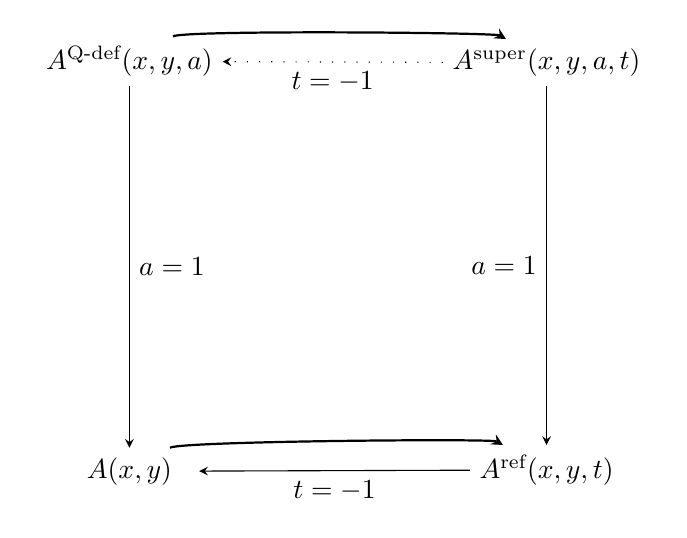
\begin{tikzpicture}
  \matrix (m) [matrix of math nodes, row sep=13em, column sep=8em, minimum width=5em]
  {
    A^{\text{Q-def}}{ (x,y,a) }  &  A^{ \text{super}}{ (x,y,a,t) }  \\
    A{ (x,y)}  &  A^{\text{ref}}{ (x,y,t)}    \\ };
  \path[-stealth]
  (m-1-1) edge[thick,bend left, looseness = 0.1] (m-1-2)
  edge node [auto] {$a=1$} (m-2-1)
  (m-1-2) edge[loosely dotted] node [below] {$t=-1$} (m-1-1)
  edge node [left] { $a=1$} (m-2-2)
  (m-2-1) edge[thick,bend left, looseness = 0.1] (m-2-2)
  (m-2-2) edge node [below] {$t = -1 $} (m-2-1);
\end{tikzpicture} 
\end{center}
\caption{ super-A-polynomials and their specializations.  Note that these are the classical limit ($q=1$) for the quantum super-A-polynomials and respective specializations into A-polynomials.} \label{Fig:superApolyspecializations}
\end{figure}

For the specialization of $q=1$, i.e. the classical limit, Conjecture 1 says that the ``large color'' behavior of the $S^{n-1}$-colored superpolynomial is related to the zero locus of the super-A-polynomial.  Thus, through the various specializations as depicted in Figure \ref{Fig:superApolyspecializations}, the relationship between the ``large color'' behavior of the corresponding knot polynomial or knot homology and corresponding deformed A-polynomial should be recovered.  Hence, the super-A-polynomial encapulates the ``large color'' behavior of a number of knot polynomials or knot homologies.  

For instance, looking at Figure \ref{Fig:superApolyspecializations} and starting from the upper-right hand corner with the super-A-polynomial $A^{\text{super}}{(x,y;a,t)}$, take the specialization $t=-1$, corresponding to decategorification.  This leads to, what was mentioned before, a $Q$-deformed A-polynomial $A^{Q-\text{def}}{(x,y;a)}$, in \cite{AganagicVafa2012}.  What should be noted is that in \cite{AganagicVafa2012}, $A^{Q-\text{def}}{(x,y;a)}$ is found to specialize to the ordinary A-polynomial of a knot for $a=1$, the quantum version $\widehat{A}^{Q-\text{def}}{(\widehat{x},\widehat{y};a,q)}$ reduces to the classical $Q$-deformed A-polynomial in the classical limit of $q\to 1$, with $a$ fixed, and $\widehat{A}^{Q-\text{def}}{(\widehat{x}, \widehat{y};a,q)}$ also obeys a quantum volume conjecture or AJ-conjecture that annihilates the colored HOMFLY-PT polynomials.  According to Conjecture 1, this $Q$-deformed A-polynomial must be contained in the super-A-polynomial as the specialization of $t=-1$, i.e. $A^{\text{super}}{ (x,y,a,t=-1)} = A^{Q-\text{ref}}{(x,y,a)}$. 
%$A^{\text{Q-def}}{ (x,y;a)}$ is the characteristic variety whose zero locus corresponds to .  $Q$-deformations correspond to extending $J_n{(K;q)}$ to higher rank knot polynomials the colored HOMFLY-PT polynomial..  According to Conjecture 1, it must be contained in  $A^{ \text{super}}{(x,y,a,t=-1)}$, as the specialization of $t=-1$.   


%the zero locus of the super-A-polynomial relates to the ``large color'' behavior of the corresponding $n$-colored superpolynomial.  Furthermore, the super-A-polynomial, in various specializations, should also encapsulate the ``large color'' behavior of the corresponding knot polynomial or knot homology.  This is depicted in Figure (\ref{Fig:superApolyspecializations}).  

%Furthermore, specializing the $Q$-deformed A-polynomial to $a=1$, $A^{\text{Q-def}}{(x,y;a)}$ reduces to the ordinary A-polynomial, possibly with some extra factors, denoted by $A(x,y)$.  

Thus, the ``classical'' super-A-polynomial $A^{\text{super}}{(x,y;a,t)}$ can be viewed as a refinement/categorification of the $Q$-deformed A-polynomial $A^{\text{Q-def}}{ (x,y;a)}$.  It can also be viewed as the ``$Q$-deformation'' of the refined A-polynomial $A^{\text{ref}}{ (x,y;t)}$, as depicted in Figure \ref{Fig:superApolyspecializations}. %Again, through Conjecture 2, there are quantum versions of each of these super-A-polynomials and their specializations, as depicted in Figure (\ref{Fig:qsuperApolyspecializations}).  

In this classical limit $q=1$, from Figure \ref{Fig:superApolyspecializations}, starting from the super-A-polynomial, the specialization $a=1$  yields the refined A-polynomial.  This could be thought of as the large color behavior of the super-A-polynomial, since if $a$ is fixed as $1$, but with $a=q^n = e^{\hbar n}$, with $\hbar \to 0$, then $n$ becomes large.  Then, specialization $t=-1$ recovers the A-polynomial.  %The $t$-deformation in this case was leading to the \emph{refined} A-polynomial.


\section{Quantum super-A-polynomials }

\subsection{Unknot}

For the case of the unknot, we only have an expression from the viewpoint of refined Chern-Simons theory for the unreduced colored superpolynomial $\overline{\mathcal{P}}_n{ (a,q,t)}$, since, by definition, reduced polynomials are normalized by the value of the unknot, so that $\mathcal{P}_n{ (\circlearrowleft; a,q,t)} =1$.  

%Despite the simplicity of the unknot, as we will see, some of the invariants for the unknot that are trivial in the non-refined and non-super case, become rather nontrivial when the $t$- or $a$- dependence is turned on.  

From \eqref{Eq:unreducedPaqtUnknotrefinedCS}, the recursion relation can be immediately written down:
\begin{equation}
\overline{\mathcal{P}}_{n+1}{ (\circlearrowleft; a,q,t) } = (-a^{-1} t^{-3} q)^{1/2} \frac{ 1 + at^3 q^{n-1}}{ 1-q^n } \overline{\mathcal{P}}_n{ (\circlearrowleft; q,t ) }
\end{equation}

Thus, according to Conjecture 2, given by \eqref{Eq:FSVolConj2b}, with $\widehat{x}=q^n$, the quantum super-A-polynomial for the unknot is the following:
\begin{equation}
  \widehat{A}^{\text{super}}{ (\widehat{x}, \widehat{y}; a,q,t) } = (-a^{-1} t^{-3} q)^{1/2} ( 1 + at^3 q^{-1}\widehat{x}) - (1-\widehat{x}) \widehat{y}
\end{equation}

In the classical limit of $q\to 1$, this quantum operator reduces to the classical super-A-polynomial:
\begin{equation}
A^{\text{super}}{ (x,y;a,t) } = {\left(x - 1\right)} y + {\left(a t^{3} x + 1\right)} \sqrt{-\frac{1}{a t^{3}}} \label{Eq:unknotsuperAp}
\end{equation}
Notice that there is no overall factor of $(y-1)$ nor $(x-1)$ with the $a$ and $t$-deformations.  

The specialization of $t=-1$, corresponding to decategorification, yields the unrefined $Q$-deformed A-polynomial for the unknot:
\begin{equation}
  A^{\text{Q-def}}{ (x,y;a) } = {\left(x - 1\right)} y - {\left(a x - 1\right)} \sqrt{\frac{1}{a}}  \label{eq:QdefApunknot}
\end{equation}

Still, $A^{\text{Q-def}}{ (x,y;a)}$ does not factorize.  When we take the limit of $a\to 1$, we reobtain the ordinary $A$-polynomial for the unknot:
\begin{equation}
  A{ (x,y)} = {\left(x - 1\right)} {\left(y - 1\right)}
\end{equation}
which factorizes into $(x-1)$ and $(y-1)$, with the $y-1$ factor describing the abelian representation for the knot group of the knot complement $M$ (as mentioned in Section \ref{Sec:Apolynomial}.

From $\widehat{A}^{\text{super}}{ (\widehat{x},\widehat{y}; a,q,t)}$, by immediately specializing to $t=-1$ for decategorification, one can also obtain the quantum version of the $Q$-deformed A-polynomial for the unknot:
\begin{equation}
  \widehat{A}^{ \text{Q-def}}{ (\widehat{x}, \widehat{y}; a,q)} = {\left(\widehat{x} - 1\right)} \widehat{y} - {\left(\frac{a \widehat{x}}{q} - 1\right)} \sqrt{\frac{q}{a}}
\end{equation}
This $\widehat{A}^{Q-\text{ref}}{(\widehat{x},\widehat{y};a,q)}$, along with its classical version \eqref{eq:QdefApunknot} is the quantum version of the $Q$-deformed A-polynomial and classical $Q$-deformed A-polynomial, respectively, found in \cite{AganagicVafa2012}.  

As an application of Conjecture 1, involving the asymptotic behavior of the colored superpolynomials for large color, \eqref{Eq:FSVolConj1b}, it would be useful to see how the super-A-polynomial for the unknot, \eqref{Eq:unknotsuperAp} is derived in this manner.  Using the asymptotic limit of the $q$-Pochhammer symbol, \eqref{Eq:qPochhammerasymptotics}, one can write down the large color limit, i.e. as $n$ or $r$ becomes large, and keeping in mind the classical limit of $q\to 1$, which means that $\hbar \to 0$ as $q = e^{\hbar}$, for the unreduced colored superpolynomial of the unknot itself: 
\begin{equation}
  \overline{\mathcal{P}}_n{ (\circlearrowleft; a,q,t) } = \exp{ \frac{1}{ \hbar}{ \left( \log{x} \log{ (-a^{-1} t^{-3} )^{1/2} } + \text{Li}_2{ (x)} - \text{Li}_2{ (-at^3x) } + \text{Li}_2{ (-at^3) } - \frac{\pi^2}{6} + \mathcal{O}{ (\hbar) } \right) } }  \label{Eq:unrefinedunknotcsPasymptotics00}
\end{equation}
with $x = q^n$ being fixed by the limit in Conjecture 1.  


%using the asymptotic analysis on \eqref{Eq:unreducedPaqtUnknotrefinedCS} according to Conjecture 1 with .  
%, $\overline{\mathcal{P}}_n$, the unreduced colored superpolynomial for the unknot, becomes in the limit given in Conjecture 1, \eqref{Eq:FSVolConj1a} \cite{bib:FGS2012}, \cite{FujiSulkowski2013}:

Thus, examining \eqref{Eq:unrefinedunknotcsPasymptotics00}, one identifies the potential $\widetilde{\mathcal{W}} = \int \log{y} \frac{dx}{x}$ in \eqref{Eq:FSVolConj1b} of Conjecture 1 to be the following:
\begin{equation}
  \widetilde{ \mathcal{W}} = \log{x} \log{ (-a^{-1} t^{-3})^{1/2} } + \text{Li}_2{(x)} - \text{Li}_2{ (-at^3)} + \text{Li}_2{ (-at^3)} - \frac{\pi^2}{6}
\end{equation}

Looking at the form of \eqref{Eq:potentialW00}, partial differentiation with respect to $x$ immediately yields an expression for $y$ in terms of the potential $\mathcal{\widetilde{W}}$ and $x$:
\begin{equation}
y = \exp{ \left( x \partial_x \widetilde{ \mathcal{W}} \right) } \label{Eq:potentialkeyidentity}
\end{equation}
with the condition that the integral was done on the zero locus of the super-A-polynomial.  So if Conjecture 1 holds true, then this identity, \eqref{Eq:potentialkeyidentity}, can be used to help find the super-A-polynomial, once the potential $\widetilde{\mathcal{W}}$.  

For the unrefined knot, one obtains
\begin{equation}
y = \exp{ \left( x \partial_x \widetilde{ \mathcal{W}} \right) } = (-a^{-1} t^{-3})^{1/2} \frac{1+ at^3 x}{ 1 - x}
\end{equation}
which reproduces \eqref{Eq:unknotsuperAp} for when $A^{\text{super}} =0$.  

\section{Quantum super-A-polynomials for Torus knots $T^{(2,2p+1)}$}

Recall that the $S^r$-colored superpolynomials, $\mathcal{P}^{S^r}{ (T^{ (2,2p+1)}; a,q,t) }$ for the torus knots $T^{(2,2p+1)}$ can be obtained from the refined Chern-Simons theory, \eqref{Eq:coloredsuperpolytorusknotrefinedCS}, and from an analysis of the differentials, \eqref{Eq:analysisofdtorusknotPr01}.  By Conjecture 2, a recursion relation can be computed, in principle, using the explicit form of $\mathcal{P}^{S^r}$.  The recursion relation was found by using the Mathematica package \texttt{qZeil.m} for \eqref{Eq:coloredsuperpolytorusknotrefinedCS}, since \eqref{Eq:coloredsuperpolytorusknotrefinedCS} involves only a single sum, and by using the Mathematica package \texttt{qMultiSum.m} for both \eqref{Eq:coloredsuperpolytorusknotrefinedCS} and \eqref{Eq:analysisofdtorusknotPr01}, since from an analysis of differentials, the explicit form of $\mathcal{P}^{S^r}$ involves more than one summation \cite{RieseqZeil}.  See Appendix \ref{app:qZeilqMultiSum} for its usage.   

While the coefficients for the quantum super-A-polynomials are collected in the Appendix \ref{app:qsAp}, here, the full expression for the quantum super-A-polynomial of the trefoil $\mathbf{3}_1$ and cinquefoil $\mathbf{5}_1$, corresponding to $p=1$ and $p=2$, for a torus knot $T^{(2,2p+1)}$, respectively, will be presented.  

Thus, for $p=1$, the quantum super-A-polynomial for the \emph{trefoil} is of the following form:

\begin{equation}
  \widehat{A}^{\text{super}}(\widehat{x}, \widehat{y}; a, q, t ) = a_0 + a_1 \widehat{y} + a_2\widehat{y}^2 \label{Eq:qsApTp01trefoil}
\end{equation}
where

\[
\begin{aligned}
  & a_0 =  \frac{a^{2} t^{4} {\left(a q t^{3} \widehat{x}^{2} + 1\right)}  {\left(\widehat{x} - 1\right)} \widehat{x}^{3}}{{\left(a t^{3} \widehat{x}^{2} + q\right)} {\left(a t^{3} \widehat{x} + 1\right)}} \\
  & a_1 = -\frac{{\left( a^2 q t^6 \widehat{x}^4+a q^2 t^5 \widehat{x}^3+ t^2 (a q^2 t  +a t  +q^3   +q^2  ) \widehat{x}^2-q^2 t^2 \widehat{x}+q\right)} {\left(a t^{3} \widehat{x}^{2} + 1\right)} a }{{\left(a t^{3} \widehat{x}^{2} + q\right)} {\left(a t^{3} \widehat{x} + 1\right)} q}  \\
  & a_2 = 1 
\end{aligned}
\]

Taking the limit $q \to 1$ of $\widehat{A}^{\text{super}}$, i.e. (\ref{Eq:qsApTp01trefoil}) above, the classical super-A-polynomial is obtained:

\begin{equation}
  A^{\text{super}}(x,y;a,t) = \frac{a^{2} t^{4} {\left(x - 1\right)} x^{3}}{a t^{3} x + 1} - \frac{ 
{\left(a^{2} t^{6} x^{4} + a t^{5} x^{3} + 2 \, a t^{3} x^{2} + 2 \, t^{2} x^{2} - t^{2} x + 1\right)} a 
    y}{a t^{3} x + 1} + y^{2}
\end{equation}

Taking $t=-1$ and $a=1$, the super-A-polynomial (\ref{Eq:qsApTp01trefoil}) reduces to the $A$-polynomial for the trefoil:

\begin{equation}
A(x,y) = {\left(x^{3} + y\right)} {\left(y - 1\right)}
\end{equation}
Note the factor of $(y-1)$ associated with the abelian representation of the knot group of the knot complement $M$, rightfully, is reproduced.  

Once again, we will examine the procedure, according to Conjecture 1, that by taking the limit given in \eqref{Eq:FSVolConj1a} and identifying the potential $\widetilde{\mathcal{W}}$ from the asymptotic limit of the colored superpolynomial $\mathcal{P}_n$, one can obtain the super-A-polynomial.  In this specific case, the trefoil will be considered, but we want to illustrate the general method.  

Now for the family of torus knots $T^{(2,2p+1)}$, there are two expressions for the colored superpolynomial, one from an analysis of differentials, which is a multiple summation, \eqref{Eq:analysisofdtorusknotPr01}, and the other from the viewpoint of refined Chern-Simons theory, which involves a single summation, \eqref{Eq:coloredsuperpolytorusknotrefinedCS}.  In a practical application of Conjecture 1, take the latter form of the colored superpolynomial.  In the large color limit, the summation over $l=0, \dots , r$ becomes an integral.  Suppose $l$ is large because ultimately we want to look at a saddle point approximation.  For the limit taken in Conjecture 1, $q\to 1$ (the classical limit) and so for $q=e^{\hbar}$, $\hbar \to 0$.  Then take $z\equiv e^{\hbar l}$ to be constant in this limit.  

Thus, as a general procedure, the colored superpolynomial in this limit becomes, after a change of variables, an integral over $z$.  

For the case of the trefoil, the colored superpolynomial $\mathcal{P}_n{ (\mathbf{3}_1;a,q,t)}$ has the following approximation as an integral in the limit specified by Conjecture 1:
\begin{equation}
\mathcal{P}_n{ (\mathbf{3}_1;a,q,t) } \sim \int dz \exp{ \left[ \frac{1}{ \hbar} \left( \widetilde{W}{ (\mathbf{3}_1;z,x)  + \mathcal{O}{ ( \hbar) } } \right) \right] }
\end{equation}

For the trefoil, the potential is the following:
\begin{equation}
  \begin{gathered}
    \widetilde{W}{ (\mathbf{3}_1;z,x) } = - \frac{ \pi^2}{ 6} + \left( \log{z} + \log{a} \right) \log{x} + 2(\log{t} )( \log{z}) + \\
    + \text{Li}_2{ (xz^{-1}) } - \text{Li}_2{(x)} + \text{Li}_2{ (-at) } - \text{Li}_2{ (-atz) } +\text{Li}_2{(z)}
\end{gathered}
\end{equation}

Recalling the key identity, \eqref{Eq:potentialkeyidentity}, $y$ is given, depending on $x$ and on $\mathcal{\widetilde{W}}$, which in this case, and for the other torus knots, depends on $x$ and $z$.  To eliminate $z$, then one takes the saddle point in $z$ for $\widetilde{\mathcal{W}}$, as was alluded to before:
\begin{equation}
  \left. \frac{ \partial \widetilde{\mathcal{W}}{ (z,x) } }{ \partial z } \right|_{z=z_0 } = 0 \label{Eq:Wpotentialsaddlepoint}
\end{equation}
\eqref{Eq:Wpotentialsaddlepoint} helps to determine the leading asymptotic behavior in \eqref{Eq:FSVolConj1b} and is used to eliminate $z$ in a system of two equations, and so to produce the super-A-polynomial. This has been done for the family of torus knots with the form of the colored superpolynomial given by the refined Chern-Simons theory \cite{bib:FGS2012}, \cite{FujiSulkowski2013}.  

Once more, quantum versions of the $Q$-deformed A-polynomial and the ordinary A-polynomial can be obtained from the quantum super-A-polynomial through a series of specializations.  Thus one obtains the following quantum versions for the trefoil:

\begin{dmath}
\widehat{A}^{\text{Q-def}}{ ( \widehat{x}, \widehat{y}; a,q) } = -\frac{{\left(a q \widehat{x}^{2} - 1\right)} a^{2} {\left(\widehat{x} - 1\right)} \widehat{x}^{3}}{{\left(a \widehat{x}^{2} - q\right)} {\left(a \widehat{x} - 1\right)}}  + \frac{ { \left( a^{2} q \widehat{x}^{4} - a q^{2} \widehat{x}^{3} - q^{2} \widehat{x} - {\left(a q^{2} - q^{3} - q^{2} + a\right)} \widehat{x}^{2} + q \right) }   {\left(a \widehat{x}^{2} - 1\right)} a \widehat{y}}{{\left(a \widehat{x}^{2} - q\right)} {\left(a \widehat{x} - 1\right)} q}   + \widehat{y}^{2}  \label{eq:qAQdeftrefoil}
\end{dmath}


\begin{dmath}
\widehat{A}{ (\widehat{x}, \widehat{y}; q ) } = -\frac{{\left(q \widehat{x}^{2} - 1\right)} \widehat{x}^{3}}{\widehat{x}^{2} - q}  + \frac{{\left(q^{3} \widehat{x}^{2} + q \widehat{x}^{4} - {\left(\widehat{x}^{2} + 1\right)} q^{2} \widehat{x} - \widehat{x}^{2} + q\right)} {\left(\widehat{x} + 1\right)} \widehat{y}}{{\left(\widehat{x}^{2} - q\right)} q   } + \widehat{y}^{2}
\end{dmath}

The quantum $Q$-deformed A-polynomial, \eqref{eq:qAQdeftrefoil}, in the classical limit $q\to 1$, reproduces the $Q$-deformed A-polynomial calculated in \cite{AganagicVafa2012}.  It annihilates the colored HOMFLY-PT polynomials. 

Once again, note the delicate issue of specializing to $a=q^2$ on the homological side versus the possibility of nontrivial differentials.  In the case of the trefoil, it was found that in the limit of $q\to 1$, $\widehat{A}^{\text{ref}}{ (\widehat{x}, \widehat{y};q,t)}$ reproduces the classical refined A-polynomial, obtained by examining the asymptotic behavior in \cite{FujiGukovSulkowski2012}.  Here is the specialization of $\widehat{A}^{\text{super}}$ for $a=q^2$:

\begin{dmath}
\widehat{A}^{\text{super}}{ (\widehat{x}, \widehat{y}; a=q^2, q,t) } = 
\frac{{\left(q t^{3} \widehat{x}^{2} + 1\right)} t^{4} {\left(\widehat{x} - 1\right)} \widehat{x}^{3}}{{\left(t^{3} \widehat{x}^{2} + q\right)} {\left(t^{3} \widehat{x} + 1\right)}}  - \frac{ { \left( q t^{6} \widehat{x}^{4} + q^{2} t^{5} \widehat{x}^{3} - q^{2} t^{2} \widehat{x} + {\left({\left(q^{2} + 1\right)} t^{3} + {\left(q^{3} + q^{2}\right)} t^{2}\right)} \widehat{x}^{2} + q \right)  }{ (t^{3} \widehat{x}^{2} + 1 ) } }{ {\left(t^{3} \widehat{x}^{2} + q\right)} {\left(t^{3} \widehat{x} + 1\right)} q }\widehat{y} + \widehat{y}^2 \label{eq:qAref00}
\end{dmath}

However, what one could do in this particular case is to compare this expression for the recursion relation directly obtained from the specialization of the colored superpolynomial, from the refined Chern-Simons theory, to the $sl{(2)}$ knot homology.  This was done in \cite{FujiGukovSulkowski2012}.  One must note that the expression for the quantum $\widehat{A}^{\text{ref}}$ in \cite{FujiGukovSulkowski2012} is in the following form:
\begin{equation}
  \widehat{A}^{\text{ref}}{ (\widehat{x}, \widehat{y};q,t) } = a_{-1} \widehat{y}^{-1} + a_0 + a_{1} \widehat{y} \label{eq:qAref01}
\end{equation}
In order to compare this expression \eqref{eq:qAref01} with the one from the quantum super-A-polynomial, \eqref{eq:qAref00}, one needs to take care to multiply by $\widehat{y}$ throughout the expression, taking heed the non-commutative nature of $\widehat{x}, \widehat{y}$ and $q$, as outlined in \eqref{eq:xycoloredsP}.  The resulting expression is the same as the specialization $a=q^2$ of $\widehat{A}^{\text{super}}$:
\begin{equation}
  \widehat{A}^{\text{super}}{ (\mathbf{3}_1; \widehat{x}, \widehat{y}; a=q^2, q,t) } = \widehat{A}^{\text{ref}}{( \mathbf{3}_1; \widehat{x}, \widehat{y}; q,t)}
\end{equation}


For $p=2$, the quantum super-A-polynomial for the \emph{cinquefoil} is of the following form: 

\begin{equation}
  \widehat{A}^{\text{super}}(\widehat{x}, \widehat{y}; a, q, t ) = a_0 + a_1 \widehat{y} + a_2\widehat{y}^2 +a_3 \widehat{y}^3   \label{Eq:qsApTp02cinquefoil}
\end{equation}
where

\begin{equation}
  a_0 = -\frac{a^6 q^3 t^{12} (\widehat{x}-1) \widehat{x}^{10} (q \widehat{x}-1) \left(a q^2 t^3 \widehat{x}^2+1\right) \left(a   q^3 t^3 \widehat{x}^2+1\right)}{\left(a t^3 \widehat{x}+1\right) \left(a t^3 \widehat{x}^2+1\right) \left(a   q t^3 \widehat{x}+1\right) \left(a t^3 \widehat{x}^2+q\right)}
\end{equation}

\begin{dmath}
  a_1 =  a^4 q t^6 \widehat{x}^5 (q \widehat{x}-1) \left(a q^3 t^3 \widehat{x}^2+1\right) 
\left( a^4 q^2 t^{10} \widehat{x}^6+a^3 q^3 t^9 \widehat{x}^5+a^2 t^6 \widehat{x}^4 \left(q^3 (a t+q+1)+a t\right)+q
   t^2 \widehat{x}^2 \left(a^2 t^2+a \left(q^4+q^3+q+1\right) t+\left(q^2+q+1\right)
   q^3\right)+a q t^5 \widehat{x}^3 \left(q^3 (a t+q+1)+a t\right)+q^2 t^2 \widehat{x} \left(a
   t-q^2\right)+q^2 (q+1)
\right)
   /  \left( \left(a t^3 \widehat{x}+1\right) \left(a q t^3 \widehat{x}+1\right) \left(a t^3
   \widehat{x}^2+q\right) \right)
\end{dmath}

\begin{dmath}
\quad \\ 
a_2 = -  
 a^2 \left(a q^2 t^3 \widehat{x}^2+1\right)  \left(
t^2 \widehat{x} \left(a^2 q^6 (q+1) t^6 \widehat{x}^5+q^3 t^2 \widehat{x}^3 \left(a^2 t^2+a
   \left(q^4+q^3+q+1\right) t+\left(q^2+q+1\right) q^3\right)+\widehat{x} \left(q^3 (a
   t+q+1)+a t\right)+a q^5 t^5 \widehat{x}^4 \left(q^2-a t\right)-q^2 t^2 \widehat{x}^2 \left(q^3 (a
   t+q+1)+a t\right)-q^2\right)+1 \right)
  / \left( q^2 \left(a t^3 \widehat{x}^2+1\right) \left(a q t^3 \widehat{x}+1\right) \right)
\end{dmath}

\begin{equation}
a_3 = 1
\end{equation}

Consider the classical limit of $q\to 1$ yielding the super-A-polynomial for the cinquefoil.  For the super-A-polynomial, 
\begin{equation}
  A^{\text{super}}{ (x,y;a,t) } = a_0 + a_1 y + a_2 y^2 + a_3y^3
\end{equation}
the following coefficients are obtained for this classical limit:

\begin{dmath}
a_0 = -\frac{a^{6} t^{12} {\left(x - 1\right)}^{2} x^{10}}{{\left(a t^{3} x + 1\right)}^{2}}
\end{dmath}

\begin{dmath*}
a_1 = \left( a^{4} t^{10} x^{6} + a^{3} t^{9} x^{5} + 2 \, {\left(a^{3} t^{7} + a^{2} t^{6}\right)} x^{4} + 2 \, {\left(a^{2} t^{6} + a t^{5}\right)} x^{3} + {\left(a^{2} t^{4} + 4 \, a t^{3} + 3 \, t^{2}\right)} x^{2} + {\left(a t^{3} - t^{2}\right)} x + 2 \right) a^4 t^6 (x-1) x^5 {\left(a t^{3} x + 1\right)}^{-2} { \left( a t^{3} x + 1 \right)^{-1} }
\end{dmath*}\begin{equation}
\end{equation}



\begin{dmath*}
a_2 = -\left( 2 \, a^{2} t^{8} x^{6} - {\left(a^{2} t^{8} - a t^{7}\right)} x^{5} + {\left(a^{2} t^{6} + 4 \, a t^{5} + 3 \, t^{4}\right)} x^{4} - 2 \, {\left(a t^{5} + t^{4}\right)} x^{3} - t^{2} x + 2 \, {\left(a t^{3} + t^{2}\right)} x^{2} + 1 \right) a^2 \left( a t^{3} x + 1 \right)^{-1}
\end{dmath*}\begin{equation}
\end{equation}


\begin{dmath}
a_3 = 1
\end{dmath}

The classical limit $q\to 1$ of the quantum super-A-polynomial $\widehat{A}^{\text{super}}{ (\widehat{x},\widehat{y};a,q,t) }$ for the cinquefoil reproduces the super-A-polynomial $A^{\text{super}}{ (x,y;a,t)}=0$, which was found by an analysis of the asymptotic behavior according to Conjecture 1 \cite{FujiGukovStosicSulkowski2013}.  

The super-A-polynomial for torus knots $T^{(2,2p+1)}$ was computed, by analyzing the asymptotics via Conjecture 1, for the cases of small $p$ \cite{bib:FGS2012}, \cite{FujiSulkowski2013}, \cite{FujiGukovStosicSulkowski2013}.  In this work, it was confirmed that the quantum super-A-polynomials for the torus knots, Appendix \ref{app:qsAp}, for the cases of $p=1$ to $p=5$, has the classical limit $q\to 1$ that coincides with the super-A-polynomials from analyzing the asymptotics.  

It should be noted that the question remains for the family of torus knots $T^{(2,2p+1)}$, whether the two expressions for the colored superpolynomial $\mathcal{P}^{ S^r}{ (T^{(2,2p+1)};a,q,t)}$, one obtained via analogue from the refined Chern-Simons theory, \eqref{Eq:coloredsuperpolytorusknotrefinedCS}, and the other obtained from analyzing the constraints imposed by the differentials, \eqref{Eq:analysisofdtorusknotPr01}, agree.  In fact, in Appendix \ref{app:qsAp}, the quantum super-A-polynomials for the torus knot $T^{(2,2p+1)}$ for the cases of $p=1, \dots , 5$ are the same when one computes a recursion relation on each \eqref{Eq:coloredsuperpolytorusknotrefinedCS} and \eqref{Eq:analysisofdtorusknotPr01}.  As seen in Conjecture 2, in \eqref{Eq:FSVolConj2b}, the quantum super-A-polynomial has its coefficients obey the recursion relation in the color index $n$, of the form \eqref{Eq:FSVolConj2a}.  Because the quantum super-A-polynomials agree in each of the two viewpoints, their colored superpolynomials also agree for all $r$.  

\subsection{The special limit of $x=1$}\label{subsec:x=1}

Consider the special limit of $x=1$.  Remember that $x=q^n$.  Also remember that in Conjecture 1, the limit was taken such that $x$ is fixed, while $q=e^{\hbar}\to 1$ and $n$ becomes large.  What one finds is the following specific relationship between the super-A-polynomial and the colored superpolynomials \cite{bib:FGS2012}, \cite{FujiSulkowski2013}, \cite{FujiGukovStosicSulkowski2013}:
\begin{equation}
A^{\text{super}}{ (x=1, y;a,t) } = y^k + y^{k-1} \mathcal{P}_{r=1}{ (a,q=1,t)}
\end{equation}
where $k$ is some integer. 

Indeed, one can take the quantum super-A-polynomials for the trefoil, cinquefoil, and the $T^{(2,7)}$ torus knot ($p=3$), as we'll do here, and the $p=4$, $p=5$ cases for the torus knots, take the classical limit $q=1$, this special limit of $x=1$ and compare the result to the colored superpolynomials, but in the specialization to $q=1$ and $r=1$ (uncolored).  So for the trefoil,
\begin{equation}
  A^{\text{super}}{ (x=1,y;a,t) } = -{\left(a^{2} t^{3} + a t^{2} + a\right)} y + y^{2} = - \mathcal{P}_{r=1}{ (a,q=1,t) }  y + y^2
\end{equation}

For the cinquefoil, 
\begin{equation}
  A^{\text{super}}{ (x=1,y;a,t) } = -{\left(a^{3} t^{5} + a^{3} t^{3} + a^{2} t^{4} + a^{2} t^{2} + a^{2}\right)} y^{2} + y^{3} = - \mathcal{P}_{r=1}{(a,q=1,t)}  y^2 + y^3
\end{equation}

For the $T^{(2,7)}$ torus knot,
\begin{equation}
  A^{\text{super}}{ (x=1,y;a,t) } = -{\left(a^{4} t^{7} + a^{4} t^{5} + a^{3} t^{6} + a^{4} t^{3} + a^{3} t^{4} + a^{3} t^{2} + a^{3}\right)} y^{3} + y^{4} = - \mathcal{P}_{r=1}{(a,q=1,t)}  y^3 + y^4
\end{equation}

Being that the colored superpolynomial is the Poincar\'{e} polynomial for the colored HOMFLY-PT knot homology, then it can be said that the super-A-polynomial knows something about the HOMFLY-PT homology, namely the dimensions of the knot homology $\mathcal{H}_{ijk}{(K)}$  

What about the quantum super-A-polynomials?  Consider that for the limit of $x=1$, for this quantum case, the case of the trefoil:
\begin{equation}
  \widehat{A}^{\text{super}}{ (\widehat{x}=1, \widehat{y};a,q,t) } = \frac{q \widehat{y}^{2} - {\left(a^{2} q t^{3} + a q^{2} t^{2} + a\right)} \widehat{y}}{q} = \widehat{y}^2 - \mathcal{P}_{r=1}{(a,q,t)} \widehat{y}
\end{equation}

For the quantum case of the cinquefoil, we have the following:
\[
 \widehat{A}^{\text{super}}{ (\widehat{x}=1 , \widehat{y}; a,q,t) } = \widehat{y}^3 + a_2(a,q,t) \widehat{y}^2   + a_1( a,q,t) \widehat{y}
\]
with the coefficients $a_1,a_2$ being the following:
{ \scriptsize
\begin{dmath}
a_1(a,q,t) = \frac{{\left(a^{3} q^{2} t^{7} + a^{2} q^{3} t^{6} + a q^{4} t^{3} + q^{5} t^{2} + a q^{3} t^{3} + q^{4} t^{2} + a^{2} t^{4} + a q t^{3} + q^{2} + q\right)} {\left(a q^{3} t^{3} + 1\right)} a^{4} {\left(q - 1\right)} q t^{6}}{{\left(a q t^{3} + 1\right)} {\left(a t^{3} + 1\right)}}
\end{dmath}

\begin{dmath}
a_2(a,q,t) =   -\left(  a^{4} q^{9} t^{10} + a^{5} q^{5} t^{9} + {\left(a^{5} q^{9} + a^{5} q^{8} - a^{5} q^{7}\right)} t^{11} + {\left(a^{4} q^{9} + a^{4} q^{8} + 2 \, a^{4} q^{6} - a^{4} q^{4}\right)} t^{8} + {\left(a^{3} q^{10} + a^{3} q^{9}\right)} t^{7} + {\left(a^{4} q^{5} + a^{4} q^{3} + a^{4} q^{2}\right)} t^{6} + {\left(a^{3} q^{7} + 2 \, a^{3} q^{6} + a^{3} q^{3} - a^{3} q^{2}\right)} t^{5} + {\left(a^{2} q^{8} + a^{2} q^{7} - a^{2} q^{5}\right)} t^{4} + {\left(a^{3} q^{3} + a^{3} q^{2} + a^{3}\right)} t^{3} + {\left(a^{2} q^{4} + a^{2} q^{3} - a^{2} q^{2}\right)} t^{2} + a^{2}   \right){     \left(   a^{2} q^{3} t^{6} + {\left(a q^{3} + a q^{2}\right)} t^{3} + q^{2}   \right)^{-1} }
\end{dmath}
}
In this case, it is unclear what the direct relationship between the quantum super-A-polynomial is to the family of colored superpolynomials.  




\section{Quantum super-A-polynomials for Twist knots }

Quantum super-A-polynomials for the twist knots $\mathbf{4}_1$, $\mathbf{5}_2$, $\mathbf{6}_1$ were calculated, using \texttt{qZeil.m} and \texttt{qMultiSum.m} Mathematica packages from the Poincar\'{e} polynomials derived from an analysis of the constraints due to differentials, given by \eqref{Eq:TwistKcoloredsuperpolynomial01}, \eqref{Eq:5_2coloredsuperpolynomial00}.  The quantum super-A-polynomials are recorded in Appendix \ref{app:qsAp}.  The classical limit $q\to 1$ of the quantum super-A-polynomials reproduce the super-A-polynomials found by an analysis of the asymptotic behavior according to Conjecture 1 \cite{FujiGukovStosicSulkowski2013}.  The quantum super-A-polynomials for the twist knots in these three cases reproduce the results obtained independently in \cite{NRZ2013}.

%Symmetry is power. Gukov




%quantum super-A-polynomials provide a good playground to discovere new things
%Piotr Su\l kowski

%Quantum curves are magical objects
%Motochico

\chapter{Conclusion} \label{ch:Conclusion}

In this work, in the Chapters \ref{chap:Field Theory}, \ref{chap:KnotTheory}, brief surveys of the Chern-Simons form, Chern-Simons gauge theory, TQFT, Witten's work on Chern-Simons theory and the Jones polynomial, basic elements of knot theory, and knot invariants were given, highlighting ingredients used for later chapters, including the colored HOMFLY-PT polynomial and A-polynomial.  A hint at the combinatorial nature of the $q$-Pochhammer symbol was given in the following chapter, Chapter \ref{chap:qPochhammersymbol}.  

The chapters on Categorification and Quantization, Chapters \ref{chap:Categorification}, \ref{chap:Quantization}, are hopefully a pedagogical-friendly review of these relatively recent developments - in particular, in the chapter on Categorification, the explicit calculation of the bi-graded (co)homology of the trefoil is a concrete example that elucidates Khovanov homology \cite{Bar-Natan2002}.  The note in the chapter on Knot Theory highlighted Reidemeister moves because proof of invariance under Reidemeister moves was essential in Khovanov's work \cite{Khovanov2000}, \cite{KhovanovRozansky2004}, \cite{KhovanovRozansky2005}.  Also in the chapter on Categorification, the colored superpolynomial was arrived at from the constraints arising from an analysis of the differentials from the triply-graded homology theory.  The generalized volume conjecture is reviewed in the chapter on Quantization.

The chapter on Refined Chern-Simons theory, \ref{chap:RefinedCStheory}, highlighted the setup for the refined topological string on $N$ M5 branes.  It also highlighted that the colored superpolynomial for the torus knots was computed by analogy to ordinary Chern-Simons theory.  In one instance, MacDonald polynomials, a two-parameter generalization of the Schur functions, became the analog in the refined theory of Schur functions that arises for the modular $S$ transformation on the space of conformal blocks for the Hilbert space.  

The new developments leading to the two main conjectures that are the main highlights in this work and the new results, namely the computation of the quantum super-A-polynomials for a few examples of the torus knots and twist knots, are in the chapter on quantum super-A-polynomials, \ref{chap:quantumsuperApolynomials}, and Appendix \ref{app:qsAp}.  

Using the Mathematica packages \texttt{qZeil.m} and \texttt{qMultiSum.m} written by Axel Riese, the recursion relations on the $S^r$-colored superpolynomials, one set of colored superpolynomials arrived at by the viewpoint of the refined Chern-Simons theory and another set of colored superpolynomials arrived at by the constraints due to an analysis of the differentials of the knot homology, were computed for the torus knots $T^{(2,2p+1)}$ for the case that $p=1, \dots, 5$ and the twist knots $\mathbf{4}_1$, $\mathbf{5}_2$, and $\mathbf{6}_1$.  The quantum super-A-polynomial arrived at from the two different viewpoints are equal for these cases.  This shows that the two different viewpoints arrive at the same colored superpolynomial.  The results also support the categorified versions of the generalized volume conjecture and the quantum volume conjecture for the colored superpolynomials proposed in \cite{bib:FGS2012}, \cite{FujiSulkowski2013}, \cite{FujiGukovSulkowski2012},  since the quantum super-A-polynomials in the classical limit of $q\to 1$ agree with the classical super-A-polynomials obtained by the asymptotic behaviors of the colored superpolynomials.  

Further investigations can include computing more cases - larger integer values of $p$ with respect to the torus knots and larger number of crossings for the twist knots - of quantum super-A-polynomials.  Not only would they help provide support for the conjectures made in \cite{bib:FGS2012}, \cite{FujiSulkowski2013}, but they would also provide a larger number of explicit examples of quantum super-A-polynomials that could help in determining the polynomial structure.  

One avenue of further investigation is to see if the quantum super-A-polynomials could be arrived by simply examining the classical super-A-polynomials and its structure, including multiplicative factors, the specific values of powers for $a,t,x$, and $y$, in the classical super-A-polynomial.  With the quantum super-A-polynomials tabulated in Appendix \ref{app:qsAp}, it is unclear what the general structure or pattern is for them.  One possible line of approach is to consider only the terms in the classical super-A-polynomial that are of the lowest order in the $a$ parameter.  Essentially, by identifying the term with the lowest power in the parameter $a$ of the classical super-A-polynomial, dividing the entire super-A-polynomial by $a$ to that power, and then letting $a \to 0$, one arrives at a super-A-polynomial in the lowest order of the $a$-parameter.  One possibility is to then observe the recursion relations that could be computed from the resulting super-A-polynomial and to surmise rules governing its transition to its quantum version.  Another way to investigate how the quantum super-A-polynomials could be arrived at from the classical super-A-polynomials is to do further analysis of the $x=1$ limit - in the most basic examples of the torus knots, specifically the trefoil, we had already seen that the classical super-A-polynomial is contained in the quantum super-A-polynomial.  

Another possible idea for additional research would be to attempt to find expressions for the colored superpolynomials of the torus knots and twist knots in other representations, other than the fundamental representation considered here \cite{NRZ2013}.  For other representations, note that the triply-graded homology with the symmetric representation is related to the antisymmetric representation via a mirror symmetry \cite{GukovStosic2012}.  Also, there may be the possibility of finding explicit forms of the colored superpolynomials of other knots and links and also colored superpolynomials of differential gauge groups.  Once the colored superpolynomials are found, the conjectures made in \cite{bib:FGS2012}, \cite{FujiSulkowski2013}, used in this work, provide a way to determine the super-A-polynomial by examining the asymptotic behavior, and the quantum super-A-polynomial, by computing a recursion relation from the colored superpolynomials.  

Finally, it would still be interesting to understand the interpretation of the $a$ and $t$-deformations in Chern-Simons gauge theory.  Along with helping to understand Khovanov homology in terms of gauge theory, it could help with understanding the \emph{framing} dependence of knot homologies \cite{bib:FGS2012}.  



\begin{appendix}

\chapter{Quantum super-A-polynomials}\label{app:qsAp}

In this appendix, the quantum super-A-polynomials for the torus knots and twist knots that were computed in this work are collected.  

\section{Torus knots, $T^{(2,2p+1)}$ }

For the following, $p$ is the positive integer.  $2p+1$ is one of the coprime integers specifying the torus knot, $(2,2p+1)$. 

%One should note that for the highest order in $\widehat{y}$, the coefficient is $1$ for each of these quantum super-A-polynomials.  The coefficient is included in the following presentation simply for completeness.  

For this appendix, the \, $\widehat{\,}$ \, notation over the operators $\widehat{x}$ and $\widehat{y}$ will be dropped for convenience. 

$p=1$. $\mathbf{3}_1$, or the \emph{Trefoil}


\begin{equation}
a_0 =   \frac{ - a^2 t^4 (1-x) x^3 \left(1 + a q t^3 x^2 \right)}{\left(1 + a t^3 x \right) \left(q + a t^3 x^2 \right)}
\end{equation}

\begin{equation}
  a_1 = -\frac{a \left( 1 + a t^3 x^2 \right) \left( q - q^2  t^2 x  + ( a q^2 t^3 +a t^3 +q^3 t^2 +q^2 t^2  ) x^2  +a q^2 t^5 x^3 + a^2 q t^6 x^4   \right) }{q \left(a t^3 x+1\right) \left(a t^3   x^2+q\right)}
\end{equation}

\begin{equation}
a_2 = 1
\end{equation}



$p=2$. $\mathbf{5}_1$ or the \emph{Cinquefoil}


\begin{equation}
  a_0 = -\frac{a^6 q^3 t^{12} (x-1) x^{10} (q x-1) \left(a q^2 t^3 x^2+1\right) \left(a   q^3 t^3 x^2+1\right)}{\left(a t^3 x+1\right) \left(a t^3 x^2+1\right) \left(a   q t^3 x+1\right) \left(a t^3 x^2+q\right)}
\end{equation}

\begin{dmath}
  a_1 =  a^4 q t^6 x^5 (q x-1) \left(a q^3 t^3 x^2+1\right) 
\left( a^4 q^2 t^{10} x^6+a^3 q^3 t^9 x^5+a^2 t^6 x^4 \left(q^3 (a t+q+1)+a t\right)+q
   t^2 x^2 \left(a^2 t^2+a \left(q^4+q^3+q+1\right) t+\left(q^2+q+1\right)
   q^3\right)+a q t^5 x^3 \left(q^3 (a t+q+1)+a t\right)+q^2 t^2 x \left(a
   t-q^2\right)+q^2 (q+1)
\right)
   /  \left( \left(a t^3 x+1\right) \left(a q t^3 x+1\right) \left(a t^3
   x^2+q\right) \right)
\end{dmath}

\begin{dmath}
\quad \\ 
a_2 = -  
 a^2 \left(a q^2 t^3 x^2+1\right)  \left(
t^2 x \left(a^2 q^6 (q+1) t^6 x^5+q^3 t^2 x^3 \left(a^2 t^2+a
   \left(q^4+q^3+q+1\right) t+\left(q^2+q+1\right) q^3\right)+x \left(q^3 (a
   t+q+1)+a t\right)+a q^5 t^5 x^4 \left(q^2-a t\right)-q^2 t^2 x^2 \left(q^3 (a
   t+q+1)+a t\right)-q^2\right)+1 \right)
  / \left( q^2 \left(a t^3 x^2+1\right) \left(a q t^3 x+1\right) \right)
\end{dmath}

\begin{equation}
a_3 = 1
\end{equation}

$p=3$:

\begin{dmath} a_0 = \frac{a^{12} q^{16} t^{24} (x-1) x^{21} (q x-1) \left(q^2 x-1\right) \left(a q^3 t^3
   x^2+1\right) \left(a q^4 t^3 x^2+1\right) \left(a q^5 t^3 x^2+1\right)}{\left(a
   t^3 x+1\right) \left(a t^3 x^2+1\right) \left(a q t^3 x+1\right) \left(a q^2 t^3
   x+1\right) \left(a t^3 x^2+q\right) \left(a q t^3 x^2+1\right)} \end{dmath}

\begin{dmath} a_1 = - \left( \left(a t^3 x+1\right) \left(a q t^3
   x+1\right) \left(a q^2 t^3 x+1\right) \left(a t^3 x^2+q\right) \left(a q t^3
   x^2+1\right)   \right)^{-1} \left(  a^9 q^{13} t^{16} x^{14} (q x-1) \left(q^2 x-1\right) \left(a q^4 t^3
   x^2+1\right) \left(a q^5 t^3 x^2+1\right) \left(a^5 t^{11} x^6+a^3 q t^7 x^4
   \left(a \left(t^3 x+t\right)+1\right)+q^7 t^2 x^2 \left(a^2 t^4 x (x+1)+a
   \left(t^3 x+t\right)+1\right)+a q^2 t^3 x^2 \left(a^2 t^4 x (x+1)+a \left(t^3
   x+t\right)+1\right)+q^3 \left(a^6 t^{14} x^8+a^2 t^4 x^2 \left(t^2 x+1\right)+a
   t^3 x (x+1)+1\right)+q^4 \left(a^5 t^{11} x^6 \left(t^2 x+1\right)+a^4 t^{10}
   x^6+a t^3 x (x+1)+1\right)+q^6 t^2 x \left(a^3 t^7 x^4+a^2 t^4 x^3 (a t+1)+a t^3
   x^2 (a t+1)+a t x+x-1\right)+q^5 \left(a^4 t^{10} x^5 (x+1)+a^3 t^7 x^4 \left(t^2
   x+1\right)+a^2 t^6 x^4+1\right)+q^8 t^2 x^2 \left(a \left(t^3
   x+t\right)+1\right)+q^9 t^2 x^2\right) \right)
\end{dmath}

\begin{dmath} a_2 = \left( \left(a t^3 x^2+1\right) \left(a q t^3 x+1\right) \left(a q^2 t^3
   x+1\right) \left(a q t^3 x^2+1\right) \right)^{-1}   \left( a^6 q^9 t^8 x^7 \left(q^2 x-1\right) \left(a q^2 t^3 x^2+1\right) \left(a q^5
   t^3 x^2+1\right) \left(q^4 t^2 x \left(a^3 t^7 x^5 (a t+1)+a t^3 x^3 (a t+1)^2-a
   t^3 x^2+a t x+x-1\right)+a^3 t^7 x^4+q^{11} t^4 x^4 \left(a^2 t^4 x^2+a \left(t^3
   x+t\right)+1\right)+a^2 t^4 x^2+q^6 t^2 x^2 \left(a^3 t^7 x^4+a^2 t^4 x^2
   \left(t^2 x+2\right)+a \left(t^3 x (2 x+1)+t\right)+2\right)-q^3 \left(a^3 t^9
   x^5+a^2 t^6 x^3+a t^5 x^3+t^2 x\right)+q \left(a^3 t^7 x^4+a^2 t^4 x^2 \left(t^2 x
   (x+1)+1\right)+a t^3 x (2 x+1)+1\right)+q^{10} t^4 x^4 \left(a^4 t^8 x^4+a^3 t^5
   x^2 \left(t^2 x+1\right)+a^2 t^4 x (2 x+1)+a t \left(t^2 x+2\right)+2\right)+q^9
   t^4 x^3 \left(a^4 t^8 x^5+a^3 t^7 x^4+2 a^2 t^4 x^3 (a t+1)+a t^3 x^2 (a t+1)+x (a
   t+1)^2-1\right)+q^8 t^4 x^3 \left(a^4 t^8 x^5+a^3 t^5 x^3+a^2 t^4 (x-1) x^2+a t
   (x-1)+x-1\right)-q^7 t^2 x^2 \left(a^4 t^{10} x^5+a^3 t^7 x^3+a^2 t^6 x^3-a t^3
   (x-1) x+t^2 x-1\right)+q^5 t^2 x^2 \left(a^4 t^8 x^4+a^3 t^5 x^2 \left(t^2 x (2
   x+1)+1\right)+a^2 t^4 x \left(t^2 x^2+4 x+1\right)+a t \left(t^2 x (2
   x+1)+2\right)+2\right)+q^2 \left(a t^3 x^2+1\right)+a t^3 x^2+q^{12} t^4
   x^4+1\right) \right)
\end{dmath}

\begin{dmath}
a_3 = - \left( q^3 \left(a q^2 t^3 x+1\right) \left(a q t^3 x^2+1\right) \right)^{-1}  \left(  a^3 \left(a q^4 t^3 x^2+1\right) \left(q^{18} t^6 x^6 \left(a^2 t^4
   x^2+1\right)+q^{17} t^6 x^6 \left(a^2 t^4 x^2+a \left(t^3
   x+t\right)+1\right)+q^{16} t^6 x^6 \left(a^2 t^4 x^2+a t+1\right)+q^{15} t^6 x^5
   \left(-a^2 t^4 x^2+a t x+x-1\right)-q^{14} t^6 x^5 \left(a^2 t^4 x^2+a
   t+1\right)+q^{12} \left(a^2 t^8 x^6+a t^7 x^6+t^4 x^4\right)+q^{11} t^4 x^4
   \left(a^2 t^4 x^2+a \left(t^3 x^2+t\right)+1\right)-q^9 \left(a^2 t^8 x^5+a t^7
   x^5+t^4 x^3\right)+q^6 \left(a^2 t^6 x^4+a t^5 x^4+t^2 x^2\right)+q^{13} t^6 x^5
   (a t (x-1)-1)+q^{10} t^4 x^4 \left(a \left(t-t^3 x\right)+1\right)-q^8 t^4 x^3 (a
   t+1)+a q^7 t^5 x^4+q^5 t^2 x^2 (a t+1)-a q^4 t^5 x^3+a q t^3 x^2-q^3 t^2
   x+1\right) \right)
\end{dmath}

\begin{dmath}
  a_4 = 1
\end{dmath}

$p=4$:

\begin{dmath}
  a_0 = -    a^{20} q^{45} t^{40} (x-1) x^{36} (q x-1) \left(q^2 x-1\right) \left(q^3
   x-1\right) \left(a q^4 t^3 x^2+1\right) \left(a q^5 t^3 x^2+1\right) \left(a q^6
   t^3 x^2+1\right) \left(a q^7 t^3 x^2+1\right)   
   \left(a t^3 x+1\right)^{-1} \left(a t^3
   x^2+1\right)^{-1} \left(a q t^3 x+1\right)^{-1} \left(a q^2 t^3 x+1\right)^{-1} \left(a q^3 t^3
   x+1\right)^{-1} \left(a t^3 x^2+q\right)^{-1} \left(a q t^3 x^2+1\right)^{-1} \left(a q^2 t^3
   x^2+1\right)^{-1}   
\end{dmath}

\begin{dmath}
a_1 = -     a^{20} q^{45} t^{40} (x-1) x^{36} (q x-1) \left(q^2 x-1\right) \left(q^3
   x-1\right) \left(a q^4 t^3 x^2+1\right) \left(a q^5 t^3 x^2+1\right) \left(a q^6
   t^3 x^2+1\right) \left(a q^7 t^3 x^2+1\right)      \left(a t^3 x+1\right)^{-1} \left(a t^3
   x^2+1\right)^{-1} \left(a q t^3 x+1\right)^{-1} \left(a q^2 t^3 x+1\right)^{-1} \left(a q^3 t^3
   x+1\right)^{-1} \left(a t^3 x^2+q\right)^{-1} \left(a q t^3 x^2+1\right)^{-1} \left(a q^2 t^3
   x^2+1\right)^{-1}
\end{dmath}


{\scriptsize
\begin{dmath}
a_2 = - a^{12} q^{36} t^{20} x^{18} \left(q^2 x-1\right) \left(q^3 x-1\right) \left(a
   t^3 x^2 q^6+1\right) \left(a t^3 x^2 q^7+1\right) \left(t^4 x^4 q^{16}+t^4 x^4
   \left(a^2 x^2 t^4+a \left(x t^3+t\right)+1\right) q^{15}+t^4 x^4 \left(a^4 x^4
   t^8+a^3 x^2 \left(x t^2+1\right) t^5+a^2 x (2 x+1) t^4+a \left(x t^2+2\right)
   t+2\right) q^{14}+t^4 x^4 \left(a^6 x^6 t^{12}+a^5 x^4 \left(x t^2+1\right)
   t^9+a^4 x^3 (2 x+1) t^8+a^3 x^2 \left(2 x t^2+3\right) t^5+a \left(2 x
   t^2+3\right) t+a^2 \left(x (3 x+2) t^4+t^2\right)+2\right) q^{13}+t^4 x^3
   \left(a^6 x^7 t^{12}+a^5 x^6 t^{11}+a^4 (2 a t+3) x^5 t^8+2 a^3 (a t+1) x^4
   t^7+a^2 \left(a^2 t^2+4 a t+3\right) x^3 t^4+a (a t x+x)^2 t^3+\left(a^2 t^2+3 a
   t+2\right) x-1\right) q^{12}+t^4 x^3 \left(a^6 x^7 t^{12}+a^5 x^5 \left(x
   t^2+2\right) t^9+a^4 x^3 \left(x (2 x+1) t^2+1\right) t^6+a^3 x^3 \left(x
   t^2+3\right) t^5+a \left(t^2 x^2+2 x-1\right) t+x+a^2 \left(2 x^3 t^4+x
   t^2\right)-1\right) q^{11}+t^2 x^2 \left(a^6 x^8 t^{14}+a^5 x^6 t^{11}+a^4 (x-1)
   x^5 t^{10}+a^3 (x-1) x^3 t^7+a^2 (x-1) x^3 t^6+a x (2 x-1) t^3+(x-1) x
   t^2+1\right) q^{10}-t^2 x^2 \left(a^6 x^7 t^{14}+a^5 x^5 t^{11}+a^4 x^5 t^{10}-a^3
   (x-1) x^3 t^7-2 a^2 x^2 t^4+x t^2-a \left(2 x^2 t^3+t\right)-2\right) q^9+t^2 x^2
   \left(a^5 x^6 t^{11}+a^4 x^4 \left(x t^2+2\right) t^8+a^3 x^2 \left(x (3 x+2)
   t^2+1\right) t^5+a^2 x \left(2 t^2 x^2+5 x+1\right) t^4+a \left(x (3 x+2)
   t^2+2\right) t+3\right) q^8+t^2 x^2 \left(a^6 x^6 t^{12}+a^5 x^4 \left(x (2 x+1)
   t^2+1\right) t^9+a^4 x^3 \left(2 t^2 x^2+5 x+1\right) t^8+a^3 x^2 \left(4 x (x+1)
   t^2+3\right) t^5+a^2 x \left(2 t^2 x^2+7 x+2\right) t^4+a \left(x (3 x+2)
   t^2+3\right) t+3\right) q^7+t^2 x \left(a^5 (a t+2) x^7 t^{11}+a^4 (a t+1) x^6
   t^{10}+a^3 \left(a^2 t^2+5 a t+3\right) x^5 t^7+a^2 (a t+1)^2 x^4 t^6+a^2 x^2
   t^4+a \left(3 a^2 t^2+5 a t+2\right) x^3 t^3+2 (a t+1) x-1\right) q^6+t^2 x
   \left(a^5 (a t+1) x^7 t^{11}+a^3 (a t+1)^2 x^5 t^7-a^3 x^4 t^7+a (a t+1)^2 x^3
   t^3-a (a t+1) x^2 t^3+a x t+x-1\right) q^5-\left(a^5 x^7 t^{13}+a^4 x^5 t^{10}+a^3
   x^5 t^9+a^2 x^3 t^6+a x^3 t^5-a x^2 t^3+x t^2-1\right) q^4+\left(a^3 x^4 t^7+a^2
   x^2 \left(x (x+1) t^2+1\right) t^4+a x (2 x+1) t^3+1\right) q^3+\left(a^5 x^6
   t^{11}+a^4 x^4 \left(x (x+1) t^2+1\right) t^8+a^3 x^3 \left(t^2 x^2+3 x+1\right)
   t^7+a^2 x^2 \left(x (x+2) t^2+2\right) t^4+a x (3 x+1) t^3+2\right) q^2+\left(a^5
   x^6 t^{11}+a^4 x^4 \left(x (x+1) t^2+1\right) t^8+a^3 x^3 (3 x+1) t^7+a^2 x^2
   \left(x (x+1) t^2+2\right) t^4+a x (2 x+1) t^3+1\right) q+a^5 t^{11} x^6+a^4 t^8
   x^4+a^3 t^7 x^4+a^2 t^4 x^2+a t^3 x^2+1\right)            \left(a q x t^3+1\right)^{-1} \left(a
   q^2 x t^3+1\right)^{-1} \left(a q^3 x t^3+1\right)^{-1} \left(a x^2 t^3+1\right)^{-1} \left(a q
   x^2 t^3+1\right)^{-1}
\end{dmath}
}


%Latex didn't like a_3

%{\scriptsize
\begin{dmath}
  a_3 =   a^8 q^{20} t^{10} x^9 \left(q^3 x-1\right) \left(a q^4 t^3 x^2+1\right)
   \left(a q^7 t^3 x^2+1\right) \left( q    \cdot   \right.
\end{dmath} \begin{dmath*}
\cdot \left(  a^4 \left(q^2+1\right)
   \left(q^2+q+1\right) q^{19} t^{14} x^{10}+a^3 \left(q^2+q+1\right) q^{17}
   t^{13} x^9 \left(q^3-a t\right)-(q+1) \left(q^2+q+1\right) q^2 t^4 x^3
   \left(-a^2 (q-1)^2 t^2+a \left(q^4-q^2+1\right) q^2
   t+q^7\right)+\left(q^2+q+1\right) t^2 x^2 \left(a^2 t^2+a
   \left(q^6+q^5+q\right) t+a t+\left(q^2+q+1\right) q^5\right)+a^2 (q+1)
   \left(q^2+q+1\right) q^{13} t^{10} x^8 \left(a^2 t^2+a
   \left(q^6+q^4-q^3+q^2+1\right) t+q^7+q^5\right)+a (q+1) q^{11} t^9 x^7
   \left(-a^3 t^3-a^2 \left(q^6+q^5-q^3+q+1\right) t^2+a \left(q^3-1\right)^2
   q^3 t+q^{10}+q^8\right)-\left(q^2+q+1\right) q^5 t^6 x^5 \left(a^3
   \left(q^4-q^2+1\right) t^3+a^2 \left(q \left(q (q+1) \left(q \left((q-1)^2
   q^2+2\right)-1\right)-1\right)+1\right) q t^2+a \left(q^6+q^5-q^3+q+1\right)
   q^5 t+q^{12}+q^{10}\right)+(q+1) \left(q^2+q+1\right) q t^4 x^4 \left(a^3
   \left((q-1) q \left(q^2+1\right)+1\right) t^3+a^2
   \left(q^8-q^7+q^5+q^4+q^3-q+1\right) q t^2+a \left(q^6+q^5+q+1\right) q^5
   t+q^{12}+q^{10}\right)+q^7 t^6 x^6 \left(a^4 \left(q^2+q+1\right) t^4+a^3
   (q+1)^4 \left((q-1) q \left(q^2+1\right)+1\right) t^3+a^2
   \left(q^2+q+1\right)^2 \left(q^8-q^7+q^5+q^4+q^3-q+1\right) q t^2+a (q+1)^2
   \left(q^2+1\right) \left(q^2+q+1\right) \left((q-1) q
   \left(q^2+1\right)+1\right) q^5 t+\left(q^2+1\right)
   \left(q^4+q^3+q^2+q+1\right) q^{10}\right)-q t^2 x \left(-a
   t+q^4+q^3+q^2\right)+q^2+q+1             \right)  +
\end{dmath*}
$         \left.  + 1  \right)    \left(a q^2 t^3 x+1\right)^{-1}
   \left(a q^3 t^3 x+1\right)^{-1} \left(a q t^3 x^2+1\right)^{-1} \left(a q^2 t^3
   x^2+1\right)^{-1} $
%}

\begin{dmath}
a_4 = -  a^4 \left(a q^6 t^3 x^2+1\right) \left(a^2 q^{33} t^{12} x^{10}+q^{32} t^8 x^8
   \left(a^2 t^4 x^2+1\right)+q^{31} t^8 x^8 \left(a^2 t^4 x^2+a \left(t^3
   x+t\right)+1\right)+q^{30} t^8 x^8 \left(a^2 t^4 x^2+a t+1\right)+q^{29} t^8 x^8
   \left(-a^2 t^4 x+a t+1\right)+q^{28} t^8 x^7 \left(-a^2 t^4 x^2+a t
   x+x-1\right)-q^{27} t^8 x^7 \left(a^2 t^4 x^2+a t+1\right)+q^{24} t^6 x^6
   \left(a^2 t^4 x^2+a t^3 x^2+1\right)+q^{23} t^6 x^6 \left(a^2 t^4 x^2+a \left(t^3
   x^2+t\right)+1\right)-q^{20} t^6 x^5 \left(a^2 t^4 x^2+a t^3 x^2+1\right)+q^{16}
   \left(a^2 t^8 x^6+a t^7 x^6+t^4 x^4\right)+q^{26} t^8 x^7 (a t (x-1)-1)+q^{25} t^8
   x^7 (a t+1) (a t x-1)+q^{22} t^6 x^6 \left(a \left(t-t^3 x\right)+1\right)-q^{21}
   t^6 x^6 (a t+1) \left(a t^3 x-1\right)-q^{19} t^6 x^5 (a t+1)+q^{18} t^6 x^5 (a t
   (x-1)-1)+a q^{17} t^7 x^6 (a t+1)+q^{15} t^4 x^4 (a t+1)+q^{14} t^4 x^4 \left(a
   \left(t-t^3 x\right)+1\right)-a q^{13} t^7 x^5 (a t+1)-q^{11} t^4 x^3 (a t+1)+a
   q^{10} t^5 x^4+a q^9 t^5 x^4 (a t+1)+q^7 t^2 x^2 (a t+1)-a q^6 t^5 x^3+a q^2 t^3
   x^2-q^{12} t^4 x^3+q^8 t^2 x^2-q^4 t^2 x+1\right)   q^{-4} \left(a q^3 t^3 x+1\right)^{-1}
   \left(a q^2 t^3 x^2+1\right)^{-1}
\end{dmath}

\begin{dmath}
a_5 = 1 
\end{dmath}

$p=5$

\begin{dmath}
  a_0 =    a^{30} q^{96} t^{60} (x-1) x^{55} (q x-1) \left(q^2 x-1\right) \left(q^3
   x-1\right) \left(q^4 x-1\right) \left(a q^5 t^3 x^2+1\right) \left(a q^6 t^3
   x^2+1\right) \left(a q^7 t^3 x^2+1\right) \left(a q^8 t^3 x^2+1\right) \left(a q^9
   t^3 x^2+1\right)       \left(a t^3 x+1\right)^{-1} \left(a t^3 x^2+1\right)^{-1} \left(a q t^3
   x+1\right)^{-1} \left(a q^2 t^3 x+1\right)^{-1} \left(a q^3 t^3 x+1\right)^{-1} \left(a q^4 t^3
   x+1\right)^{-1} \left(a t^3 x^2+q\right)^{-1} \left(a q t^3 x^2+1\right)^{-1} \left(a q^2 t^3
   x^2+1\right)^{-1} \left(a q^3 t^3 x^2+1\right)^{-1}
\end{dmath}

\begin{dmath}
a_1 = -   a^{25} q^{91} t^{48} x^{44} (q x-1) \left(q^2 x-1\right) \left(q^3 x-1\right)
   \left(q^4 x-1\right) \left(a t^3 x^2 q^6+1\right) \left(a t^3 x^2 q^7+1\right)
   \left(a t^3 x^2 q^8+1\right) \left(a t^3 x^2 q^9+1\right) \left(a^9 x^{10}
   t^{19}+a^7 q x^8 \left(a \left(x t^3+t\right)+1\right) t^{15}+a^5 q^2 x^6
   \left(a^2 x (x+1) t^4+a \left(x t^3+t\right)+1\right) t^{11}+a^3 q^3 x^4 \left(a^3
   x^2 \left(x t^2+1\right) t^5+a^2 x (x+1) t^4+a \left(x t^3+t\right)+1\right) t^7+a
   q^4 x^2 \left(a^4 x^3 (x+1) t^8+a^3 x^2 \left(x t^2+1\right) t^5+a^2 x (x+1) t^4+a
   \left(x t^3+t\right)+1\right) t^3+q^{15} x^2 t^2+q^{10} x \left(a^5 x^6 t^{11}+a^4
   (a t+1) x^5 t^8+a^3 (a t+1) x^4 t^7+a^2 (a t+1) x^3 t^4+a (a t+1) x^2 t^3+a x
   t+x-1\right) t^2+q^{14} x^2 \left(a \left(x t^3+t\right)+1\right) t^2+q^{13} x^2
   \left(a^2 x (x+1) t^4+a \left(x t^3+t\right)+1\right) t^2+q^{12} x^2 \left(a^3 x^2
   \left(x t^2+1\right) t^5+a^2 x (x+1) t^4+a \left(x t^3+t\right)+1\right)
   t^2+q^{11} x^2 \left(a^4 x^3 (x+1) t^8+a^3 x^2 \left(x t^2+1\right) t^5+a^2 x
   (x+1) t^4+a \left(x t^3+t\right)+1\right) t^2+q^5 \left(a^{10} x^{12} t^{22}+a^4
   x^4 \left(x t^2+1\right) t^8+a^3 x^3 (x+1) t^7+a^2 x^2 \left(x t^2+1\right) t^4+a
   x (x+1) t^3+1\right)+q^9 \left(a^6 x^7 (x+1) t^{14}+a^5 x^6 \left(x t^2+1\right)
   t^{11}+a^4 x^5 (x+1) t^{10}+a^3 x^4 \left(x t^2+1\right) t^7+a^2 x^4
   t^6+1\right)+q^7 \left(a^8 x^9 (x+1) t^{18}+a^7 x^8 \left(x t^2+1\right)
   t^{15}+a^6 x^8 t^{14}+a^2 x^2 \left(x t^2+1\right) t^4+a x (x+1) t^3+1\right)+q^8
   \left(a^7 x^8 \left(x t^2+1\right) t^{15}+a^6 x^7 (x+1) t^{14}+a^5 x^6 \left(x
   t^2+1\right) t^{11}+a^4 x^6 t^{10}+a x (x+1) t^3+1\right)+q^6 \left(a^9 x^{10}
   \left(x t^2+1\right) t^{19}+a^8 x^{10} t^{18}+a^3 x^3 (x+1) t^7+a^2 x^2 \left(x
   t^2+1\right) t^4+a x (x+1) t^3+1\right)\right)       \left(a x t^3+1\right)^{-1} \left(a q x
   t^3+1\right)^{-1} \left(a q^2 x t^3+1\right)^{-1} \left(a q^3 x t^3+1\right)^{-1} \left(a t^3 x
   q^4+1\right)^{-1} \left(a x^2 t^3+q\right)^{-1} \left(a q x^2 t^3+1\right)^{-1} \left(a q^2 x^2
   t^3+1\right)^{-1} \left(a q^3 x^2 t^3+1\right)^{-1}
\end{dmath}

{\scriptsize
\begin{dmath}
     a_2 =    a^{20} q^{85} t^{36} x^{33} \left(q^2 x-1\right) \left(q^3 x-1\right) \left(q^4
   x-1\right) \left(a t^3 x^2 q^7+1\right) \left(a t^3 x^2 q^8+1\right) \left(a t^3
   x^2 q^9+1\right) \left(t^4 x^4 q^{20}+t^4 x^4 \left(a^2 x^2 t^4+a \left(x
   t^3+t\right)+1\right) q^{19}+t^4 x^4 \left(a^4 x^4 t^8+a^3 x^2 \left(x
   t^2+1\right) t^5+a^2 x (2 x+1) t^4+a \left(x t^2+2\right) t+2\right) q^{18}+t^4
   x^4 \left(a^6 x^6 t^{12}+a^5 x^4 \left(x t^2+1\right) t^9+a^4 x^3 (2 x+1) t^8+a^3
   x^2 \left(2 x t^2+3\right) t^5+a \left(2 x t^2+3\right) t+a^2 \left(x (3 x+2)
   t^4+t^2\right)+2\right) q^{17}+t^4 x^4 \left(a^8 x^8 t^{16}+a^7 x^6 \left(x
   t^2+1\right) t^{13}+a^6 x^5 (2 x+1) t^{12}+a^5 x^4 \left(2 x t^2+3\right) t^9+a^4
   x^2 \left(x (4 x+3) t^2+1\right) t^6+a^3 x \left(3 t^2 x^2+5 x+1\right) t^5+2 a
   \left(x t^2+2\right) t+a^2 \left(x (4 x+3) t^4+t^2\right)+3\right) q^{16}+t^4 x^3
   \left(a^8 x^9 t^{16}+a^7 x^8 t^{15}+a^6 (2 a t+3) x^7 t^{12}+a^5 (2 a t+3) x^6
   t^{11}+a^4 \left(a^2 t^2+5 a t+4\right) x^5 t^8+a^3 \left(a^2 t^2+4 a t+3\right)
   x^4 t^7+2 a^2 \left(a^2 t^2+3 a t+2\right) x^3 t^4+a \left(a^2 t^2+3 a t+2\right)
   x^2 t^3+2 (a t+1)^2 x-1\right) q^{15}+t^4 x^3 \left(a^8 x^9 t^{16}+a^7 x^7 \left(x
   t^2+2\right) t^{13}+a^6 x^5 \left(x (3 x+2) t^2+1\right) t^{10}+a^5 x^4 \left(2
   t^2 x^2+5 x+1\right) t^9+a^4 x^3 \left(x (4 x+3) t^2+2\right) t^6+a^3 x^2 \left(2
   t^2 x^2+5 x+1\right) t^5+a^2 x \left(x (3 x+1) t^2+1\right) t^2+a \left(t^2 x^2+3
   x-1\right) t+2 x-1\right) q^{14}+t^2 x^2 \left(a^8 x^{10} t^{18}+a^7 x^9 t^{17}+2
   a^7 x^8 t^{15}+a^6 x^7 (2 x+1) t^{14}+a^5 x^7 t^{13}+a^6 x^6 t^{12}+3 a^5 x^6
   t^{11}+2 a^4 x^6 t^{10}+a^3 x^5 t^9+a^4 x^4 t^8+a^3 x^3 (3 x-1) t^7+2 a^2 x^4
   t^6+a x^3 t^5+a^2 x^2 t^4+a x (3 x-1) t^3+(x-1) x t^2+1\right) q^{13}+t^2 x^2
   \left(a^8 x^{10} t^{18}+a^7 x^8 t^{15}+a^6 (x-1) x^7 t^{14}+a^5 (x-1) x^5
   t^{11}+a^4 (x-1) x^5 t^{10}+a^3 x^3 (2 x-1) t^7+a^2 x^2 \left(t^2 x^2+2\right)
   t^4+(x-1) x t^2+a \left(3 x^2 t^3+t\right)+2\right) q^{12}+t^2 x^2 \left(-a^8 x^9
   t^{18}-a^7 x^7 t^{15}-a^6 x^7 t^{14}+a^5 (x-1) x^5 t^{11}+2 a^4 x^4 t^8+a^3 x^2
   \left(x (3 x+1) t^2+1\right) t^5+a^2 x \left(t^2 x^2+5 x+1\right) t^4-x t^2+a
   \left(x (3 x+1) t^2+2\right) t+3\right) q^{11}+t^2 x^2 \left(a^7 x^8 t^{15}+a^6
   x^6 \left(x t^2+2\right) t^{12}+a^5 x^4 \left(x (3 x+2) t^2+1\right) t^9+a^4 x^3
   \left(3 t^2 x^2+6 x+1\right) t^8+a^3 x^2 \left(5 x (x+1) t^2+3\right) t^5+a^2 x
   \left(3 t^2 x^2+8 x+2\right) t^4+a \left(x (4 x+3) t^2+3\right) t+4\right)
   q^{10}+t^2 x^2 \left(a^8 x^8 t^{16}+a^7 x^6 \left(x (2 x+1) t^2+1\right)
   t^{13}+a^6 x^5 \left(2 t^2 x^2+5 x+1\right) t^{12}+a^5 x^4 \left(5 x (x+1)
   t^2+3\right) t^9+a^4 x^3 \left(4 t^2 x^2+10 x+3\right) t^8+a^3 x^2 \left(x (6 x+7)
   t^2+5\right) t^5+a^2 x \left(3 t^2 x^2+10 x+3\right) t^4+a \left(x (4 x+3)
   t^2+4\right) t+4\right) q^9+t^2 x \left(a^7 (a t+2) x^9 t^{15}+a^6 (a t+2) x^8
   t^{14}+a^5 \left(a^2 t^2+6 a t+5\right) x^7 t^{11}+a^4 \left(a^2 t^2+5 a
   t+3\right) x^6 t^{10}+a^3 \left(4 a^2 t^2+10 a t+5\right) x^5 t^7+a^2 \left(3 a^2
   t^2+5 a t+2\right) x^4 t^6+a \left(5 a^2 t^2+8 a t+3\right) x^3 t^3+a (2 a t+1)
   x^2 t^3+3 (a t+1) x-1\right) q^8+t^2 x \left(a^7 (a t+2) x^9 t^{15}+a^6 (a t+1)
   x^8 t^{14}+a^5 \left(a^2 t^2+5 a t+3\right) x^7 t^{11}+a^4 (a t+1)^2 x^6 t^{10}+3
   a^3 (a t+1)^2 x^5 t^7+a^2 \left(a^2 t^2+a t+1\right) x^4 t^6+a \left(3 a^2 t^2+5 a
   t+2\right) x^3 t^3+2 (a t+1) x-1\right) q^7+\left(a^8 x^{10} t^{18}+a^7 x^{10}
   t^{17}+a^7 x^8 t^{15}+2 a^6 x^8 t^{14}+a^5 (x-1) x^7 t^{13}+a^5 x^6 t^{11}+a^4 x^5
   (2 x-1) t^{10}+a^3 (x-1) x^5 t^9+a^3 x^4 t^7+a^2 x^3 (2 x-1) t^6+a (x-1) x^3 t^5+2
   a x^2 t^3+(x-1) x t^2+1\right) q^6-\left(a^7 x^9 t^{17}+a^6 x^7 t^{14}+a^5 x^7
   t^{13}+a^4 x^5 t^{10}+a^3 x^5 t^9-a^3 x^4 t^7-a^2 x^4 t^6+a x^3 t^5-a^2 x^2 t^4-a
   x (2 x+1) t^3+x t^2-1\right) q^5+\left(a^5 x^6 t^{11}+a^4 x^4 \left(x (x+1)
   t^2+1\right) t^8+a^3 x^3 \left(t^2 x^2+3 x+1\right) t^7+a^2 x^2 \left(x (x+2)
   t^2+2\right) t^4+a x (3 x+1) t^3+2\right) q^4+\left(a^7 x^8 t^{15}+a^6 x^6 \left(x
   (x+1) t^2+1\right) t^{12}+a^5 x^5 \left(t^2 x^2+3 x+1\right) t^{11}+a^4 x^4
   \left(x (2 x+3) t^2+2\right) t^8+a^3 x^3 \left(t^2 x^2+5 x+2\right) t^7+a^2 x^2
   \left(x (2 x+3) t^2+3\right) t^4+2 a x (2 x+1) t^3+2\right) q^3+\left(a^7 x^8
   t^{15}+a^6 x^6 \left(x (x+1) t^2+1\right) t^{12}+a^5 x^5 \left(t^2 x^2+4
   x+1\right) t^{11}+a^4 x^4 \left(x (2 x+3) t^2+3\right) t^8+a^3 x^3 \left(t^2 x^2+5
   x+2\right) t^7+a^2 x^2 \left(x (x+2) t^2+3\right) t^4+a x (3 x+1) t^3+2\right)
   q^2+\left(a^7 x^8 t^{15}+a^6 x^6 \left(x (x+1) t^2+1\right) t^{12}+a^5 x^5 (3 x+1)
   t^{11}+a^4 x^4 \left(x (x+1) t^2+2\right) t^8+a^3 x^3 (3 x+1) t^7+a^2 x^2 \left(x
   (x+1) t^2+2\right) t^4+a x (2 x+1) t^3+1\right) q+a^7 t^{15} x^8+a^6 t^{12}
   x^6+a^5 t^{11} x^6+a^4 t^8 x^4+a^3 t^7 x^4+a^2 t^4 x^2+a t^3 x^2+1\right)         \left(a
   q x t^3+1\right)^{-1} \left(a q^2 x t^3+1\right)^{-1} \left(a q^3 x t^3+1\right)^{-1} \left(a t^3
   x q^4+1\right)^{-1} \left(a x^2 t^3+1\right)^{-1} \left(a q x^2 t^3+1\right)^{-1} \left(a q^3 x^2
   t^3+1\right)^{-1}           
\end{dmath}   }



% p=5
{\tiny
\begin{dmath}
a_3=  - a^{15} q^{65} t^{24} x^{22} \left(q^3 x-1\right) \left(q^4 x-1\right) \left(a
   t^3 x^2 q^4+1\right) \left(a t^3 x^2 q^8+1\right) \left(a t^3 x^2 q^9+1\right)
   \left(t^6 x^6 \left(a^6 x^6 t^{12}+a^4 x^4 t^8+a^2 x^2 t^4+1\right) q^{30}+t^6 x^6
   \left(a^6 x^6 t^{12}+a^5 x^4 \left(x t^2+1\right) t^9+2 a^4 x^4 t^8+a^3 x^2
   \left(x t^2+1\right) t^5+2 a^2 x^2 t^4+a \left(x t^3+t\right)+1\right) q^{29}+t^6
   x^6 \left(2 a^6 x^6 t^{12}+a^5 x^4 \left(x t^2+2\right) t^9+a^4 x^3 (4 x+1)
   t^8+a^3 x^2 \left(2 x t^2+3\right) t^5+a^2 x (4 x+1) t^4+a \left(x t^2+2\right)
   t+2\right) q^{28}+t^6 x^6 \left(2 a^6 x^6 t^{12}+2 a^5 x^4 \left(x t^2+2\right)
   t^9+a^4 x^2 \left(x (5 x+2) t^2+1\right) t^6+3 a^3 x^2 \left(x t^2+2\right) t^5+2
   a \left(x t^2+2\right) t+a^2 \left(x (5 x+2) t^4+t^2\right)+3\right) q^{27}+t^6
   x^6 \left(2 a^6 x^6 t^{12}+a^5 x^4 \left(x t^2+4\right) t^9+a^4 x^2 \left(x (5
   x+3) t^2+2\right) t^6+a^3 x \left(3 t^2 x^2+8 x+1\right) t^5+a^2 \left(3 x (2 x+1)
   t^2+2\right) t^2+a \left(2 x t^2+5\right) t+3\right) q^{26}+t^6 x^5 \left(a^6 x^7
   t^{12}+a^5 (1-a t) x^6 t^{11}+4 a^4 (a t+1) x^5 t^8+a^3 (a t+2) x^4 t^7+a^2
   \left(3 a^2 t^2+8 a t+5\right) x^3 t^4+a \left(a^2 t^2+2 a t+2\right) x^2 t^3+3 (a
   t+1)^2 x-1\right) q^{25}+t^6 x^5 \left(a^6 (x-1) x^6 t^{12}+a^5 x^4 (2 x-1)
   t^9+a^4 x^3 \left(x (2 x-1) t^2+2\right) t^6+a^2 x \left(4 t^2 x^2+3\right) t^2+a
   \left(t^2 x^2+5 x-1\right) t+3 x+a^3 \left(x^4 t^7+6 x^3 t^5+x t^3\right)-1\right)
   q^{24}+t^6 x^5 \left(-a^6 x^6 t^{12}+2 a^5 (x-1) x^4 t^9+a^4 x^3 \left((x-3) x
   t^2+1\right) t^6+a^3 x^2 (4 x-3) t^5+2 a^2 x \left((x-1) x t^2+1\right) t^2+a
   \left(t^2 x^2+5 x-2\right) t+2 (x-1)\right) q^{23}+t^4 x^4 \left(-a^6 x^7
   t^{14}+a^6 x^6 t^{12}+2 a^5 (x-1) x^5 t^{11}-a^4 x^5 t^{10}+a^4 x^3 (2 x-1) t^8+4
   a^3 (x-1) x^3 t^7+a^2 (x-2) x^3 t^6+a^2 x (3 x-1) t^4+a x (4 x-3) t^3+(x-2) x
   t^2+1\right) q^{22}+t^4 x^4 \left(2 a^6 x^6 t^{12}+a^5 x^4 \left(4 t^2
   x^2+1\right) t^9+a^4 x^3 \left(t^2 x^2+6 x-1\right) t^8+a^3 x^2 \left(x (6 x-1)
   t^2+1\right) t^5+a^2 x (6 x-1) t^4+(x-2) x t^2+a \left(x (5 x-2)
   t^3+t\right)+2\right) q^{21}+t^4 x^4 \left(3 a^6 x^6 t^{12}+a^5 x^4 \left(2 x (2
   x+1) t^2+3\right) t^9+a^4 x^3 \left(3 t^2 x^2+12 x+1\right) t^8+a^3 x^2 \left(4 x
   (2 x+1) t^2+5\right) t^5+2 a^2 x^2 \left(x t^2+6\right) t^4-x t^2+a \left(5 t^2
   x^2+3\right) t+4\right) q^{20}+t^4 x^4 \left(3 a^6 x^6 t^{12}+a^5 x^4 \left(2 x (2
   x+1) t^2+5\right) t^9+a^4 x^2 \left(2 x^3 t^4+x (14 x+3) t^2+1\right) t^6+a^3 x^2
   \left(x (8 x+7) t^2+10\right) t^5-x t^2+2 a \left(x (3 x+1) t^2+3\right) t+a^2
   \left(3 x^3 t^6+x (16 x+3) t^4+t^2\right)+5\right) q^{19}+t^4 x^4 \left(2 a^6 x^6
   t^{12}+a^5 x^4 \left(2 t^2 x^2+5\right) t^9+a^4 x^2 \left(x^3 t^4+3 x (4 x+1)
   t^2+2\right) t^6+a^3 x \left(6 t^2 x^3+4 t^2 x^2+13 x+1\right) t^5+a \left(x (5
   x+2) t^2+8\right) t+2 a^2 \left(x^3 t^6+2 x (4 x+1) t^4+t^2\right)+6\right)
   q^{18}+t^4 x^3 \left(a^5 (a t+1) x^7 t^{11}-a^5 (a t+2) x^6 t^{11}+3 a^3 (a t+1)^2
   x^5 t^7-a^2 \left(a^2 t^2+a t-1\right) x^4 t^6+a^2 (a t+1) x^2 t^4+2 a \left(a^3
   t^3+5 a^2 t^2+6 a t+2\right) x^3 t^3+\left(3 a^2 t^2+8 a t+5\right) x-1\right)
   q^{17}+t^4 x^3 \left(-a^6 x^6 t^{12}+a^5 x^4 \left(-2 t^2 x^2+x-1\right) t^9+a^4
   x^3 \left(x (2 x-5) t^2+1\right) t^6+a^3 x^2 \left(t^2 x^3-4 t^2 x^2+5 x-1\right)
   t^5+2 a^2 x \left(x (3 x-2) t^2+1\right) t^2+a \left(2 t^2 x^3-2 t^2 x^2+6
   x-1\right) t+4 x-2\right) q^{16}+t^4 x^3 \left(-a^6 x^6 t^{12}-a^5 x^4 \left(t^2
   x^2-x+1\right) t^9+a^4 (x-5) x^4 t^8+a^3 x^2 \left(-3 t^2 x^2+2 x-3\right) t^5+a^2
   x \left(x (3 x-7) t^2+1\right) t^2+a \left(t^2 x^3-3 t^2 x^2+4 x-2\right) t+2
   x-3\right) q^{15}+t^2 x^2 \left(a^6 x^6 t^{12}+a^5 x^5 (3 x-1) t^{11}+a^4 x^5 (2
   x-1) t^{10}+2 a^4 x^4 t^8+a^3 x^3 (5 x-3) t^7+2 a^2 (x-2) x^3 t^6-2 a x^3 t^5+2
   a^2 x^2 t^4+a x (4 x-3) t^3+(x-3) x t^2+1\right) q^{14}+t^2 x^2 \left(a^6 x^6
   t^{12}+a^5 x^4 \left(x (5 x+1) t^2+1\right) t^9+3 a^4 x^4 \left(x (x+1)
   t^2+2\right) t^8+a^3 x^2 \left(x^3 t^4+x (10 x+1) t^2+1\right) t^5+a^2 x^2 \left(x
   (3 x+1) t^2+6\right) t^4-2 x t^2+a \left(-x^3 t^5+x (6 x-1) t^3+t\right)+2\right)
   q^{13}+t^2 x^2 \left(2 a^6 x^6 t^{12}+a^5 x^4 \left(x (5 x+1) t^2+1\right) t^9+a^4
   x^3 \left(2 t^2 x^3+3 t^2 x^2+10 x+1\right) t^8+a^3 x^2 \left(x^3 t^4+x (13 x+5)
   t^2+3\right) t^5+a^2 x \left(3 t^2 x^3+4 t^2 x^2+12 x+1\right) t^4-x t^2+a \left(x
   (8 x+1) t^2+2\right) t+4\right) q^{12}+t^2 x^2 \left(a^6 x^6 t^{12}+a^5 x^4
   \left(x (3 x+1) t^2+2\right) t^9+a^4 x^3 \left(t^2 x^3+t^2 x^2+10 x+1\right) t^8+5
   a^3 x^2 \left(x (2 x+1) t^2+1\right) t^5+a^2 x \left(2 t^2 x^3+3 t^2 x^2+14
   x+2\right) t^4+a \left(x (8 x+3) t^2+4\right) t+5\right) q^{11}+t^2 x^2 \left(a^6
   x^6 t^{12}+a^5 x^4 \left((x-1) x t^2+1\right) t^9+a^4 x^3 \left(-t^2 x^2+6
   x+1\right) t^8+a^3 x^2 \left(x (5 x+1) t^2+5\right) t^5+a^2 x \left(t^2 x^3+12
   x+2\right) t^4+a \left(x (6 x+1) t^2+4\right) t+5\right) q^{10}-t^2 x \left(a^4 (a
   t+1) x^6 t^{10}-a^3 (a t+1)^2 x^5 t^7+a^2 \left(a^2 t^2+3 a t+1\right) x^4 t^6-3 a
   (a t+1)^2 x^3 t^3+a x^2 t^3-4 (a t+1) x+1\right) q^9-t^2 x \left(a^5 x^6
   t^{11}+a^2 \left(a^2 t^2+3 a t+1\right) x^4 t^6-a (a t+1)^2 x^3 t^3+a (2 a t+3)
   x^2 t^3-2 (a t+1) x+1\right) q^8+t^2 x \left(a^4 (a t+1) x^5 t^8-a^3 (a t+1) x^4
   t^7+a^2 (a t+1) x^3 t^4-2 a (a t+1) x^2 t^3+2 a x t+x-2\right) q^7+\left(a^5 x^6
   t^{11}+a^4 x^5 (2 x+1) t^{10}+a^3 x^5 (x+1) t^9+a^4 x^4 t^8+3 a^3 x^4 t^7+2 a^2
   x^4 t^6-a x^3 t^5+a^2 x^2 t^4+2 a x^2 t^3-x t^2+1\right) q^6+\left(2 a^5 x^6
   t^{11}+a^4 x^5 (2 x+1) t^{10}+a^3 x^5 t^9+a^4 x^4 t^8+a^3 x^3 (5 x+1) t^7+a^2 x^3
   (3 x+2) t^6+2 a^2 x^2 t^4+a x (4 x+1) t^3-x t^2+1\right) q^5+\left(a^5 x^6
   t^{11}+a^4 x^4 \left(x (x+1) t^2+2\right) t^8+a^3 x^3 (5 x+1) t^7+a^2 x^2 \left(2
   x (x+1) t^2+3\right) t^4+a x (4 x+1) t^3+2\right) q^4+\left(a^5 x^6 t^{11}+a^4 x^4
   t^8+a^3 x^3 (3 x+1) t^7+a^2 x^2 \left(x (x+1) t^2+3\right) t^4+a x (4 x+1)
   t^3+2\right) q^3+\left(a^4 x^4 t^8+a^3 x^4 t^7+2 a^2 x^2 t^4+a x (2 x+1)
   t^3+2\right) q^2+\left(a^2 x^2 t^4+a x^2 t^3+1\right) q+1\right)      \left(a q^2 x
   t^3+1\right)^{-1} \left(a q^3 x t^3+1\right)^{-1} \left(a t^3 x q^4+1\right)^{-1} \left(a q x^2
   t^3+1\right)^{-1} \left(a q^2 x^2 t^3+1\right)^{-1} \left(a q^3 x^2 t^3+1\right)^{-1}
\end{dmath}
}

\pagebreak


\begin{dmath}
a_4 =   a^{10} q^{35} t^{12} x^{11} \left(q^4 x-1\right) \left(a t^3 x^2 q^6+1\right) \left(a t^3 x^2 q^9+1\right) \left( q \left( q \cdot \right. \right.
   \end{dmath}
\begin{dmath*}
%\left(q \left(q 
\cdot  \left(a^4 \left(q^2+1\right) \left(q^4+q^3+q^2+q+1\right) t^{16} x^{12} q^{34}+a^3
   \left(q^2+1\right) t^{15} \left(q^4 (q+1)-a \left(q^2+q+1\right) t\right) x^{11} q^{31}+a^2 (q+1)
   \left(q^2+1\right) t^{12} \left(\left(q^4+q^3+q^2+q+1\right) q^6+a^2 \left(q^2+q+1\right) t^2+a \left(q \left(q
   (q+1) \left(q^6+q^4+1\right)+1\right)+1\right) t\right) x^{10} q^{26}+a t^{11}
   \left(\left(q^4+q^3+q^2+q+1\right) q^{10}+a (q+1) \left(q^2+1\right) \left((q+1) \left((q-1) q^2-1\right)
   q^2+1\right) t q^4-a^3 (q+1) \left(q^2+q+1\right) t^3-a^2 \left(q^2+q+1\right) \left(q (q+1)
   \left(\left(q^3+q-1\right) q^3+1\right)+1\right) t^2\right) x^9 q^{23}+t^8 \left(((q-1) q+1)
   \left(q^2+q+1\right) \left(q^4+q^3+q^2+q+1\right) q^{12}+a \left(q^2+1\right)^2 \left(q \left(q^8+2
   q^7+q^6+q^4+q^3+q+2\right)+1\right) t q^6+a^2 \left(q^2+1\right)^2 \left(q (q+1) \left(q^2+q+1\right) \left(q
   \left(q^7-q^6+q^3+q^2+q-2\right)+1\right)+1\right) t^2 q+a^4 \left(q^2+q+1\right)^2 t^4+a^3
   \left(q^2+q+1\right)^2 \left(q^7+q^6+q+1\right) t^3\right) x^8 q^{18}-t^8 \left(\left(q^2+1\right)
   \left(q^4+q^3+q^2+q+1\right) q^{12}+a (q+1) \left(q^2+1\right) \left(q (q+1) \left(\left(q^3+q-1\right)
   q^3+1\right)+1\right) t q^6+a^2 \left(q^2+q+1\right) \left(\left(q^2+q+1\right) \left(q^7-q^6+2 q^2+q-1\right)
   q^3+1\right) t^2 q+a^4 \left(q^2+q+1\right) t^4+a^3 (q+1) \left(q \left(q (q+1)
   \left(q^5+q^4-q+1\right)+2\right)+1\right) t^3\right) x^7 q^{15}+(q+1) \left(q^2+1\right) t^6
   \left(\left(q^4+q^3+q^2+q+1\right) q^{12}+a (q+1) \left(q^2+1\right) \left(q^2+q+1\right)
   \left(q^4-q^2+1\right) t q^6+a^2 \left(q^{12}+q^{11}-q^9+3 q^7+4 q^6+3 q^5-q^3+q+1\right) t^2 q+a^4 t^4+a^3
   (q+1) \left(q^2+q+1\right) \left(q^4-q^2+1\right) t^3\right) x^6 q^{10}-t^6 \left((q+1) \left(q^2+1\right)
   \left(q^2+q+1\right) q^{12}+a \left(q^2+q+1\right) \left(q \left(q (q+1)
   \left(q^5+q^4-q+1\right)+2\right)+1\right) t q^6+a^2 (q+1) \left(\left(q^2+q+1\right) \left(q^7-q^6+2
   q^2+q-1\right) q^3+1\right) t^2 q+a^3 \left(q (q+1) \left(\left(q^3+q-1\right) q^3+1\right)+1\right) t^3\right)
   x^5 q^7-t^4 \left(\left(q^2+q+1\right)^2 q^8+a (q+1) \left(q (q+1) \left(\left(q^3+q-1\right)
   q^3+1\right)+1\right) t q^2+a^2 \left(-q^6+q^4+q^3+q^2-1\right) t^2\right) x^3 q^3+\left(q^2+1\right) t^4
   \left(\left(q^2+q+1\right)^2 q^{12}+a (q+1) \left(q^2+q+1\right)^2 \left(q^4-q^2+1\right) t q^6+a^2 \left(q
   (q+1) \left(q^2+q+1\right) \left(q \left(q^7-q^6+q^3+q^2+q-2\right)+1\right)+1\right) t^2 q+a^3
   \left(q^7+q^6+q+1\right) t^3\right) x^4 q^2+q^2-t^2 \left(q^5+q^4+q^3+q^2-a t\right) x q+q+(q+1)
   \left(q^2+1\right) t^2 \left(\left(q^2+q+1\right) q^6+a^2 t^2+a \left(q^7+q^6+q+1\right) t\right)
   x^2+1\right) +  
\end{dmath*}
\begin{dmath*}
\left. \left.  +1\right)+1\right)        \left(a q^3 x t^3+1\right)^{-1} \left(a t^3 x q^4+1\right)^{-1} \left(a q^2 x^2
   t^3+1\right)^{-1}   \left(a q^3 x^2 t^3+1\right)^{-1}
\end{dmath*}


\begin{dmath}
a_5 = -   a^5 \left(a t^3 x^2 q^8+1\right) \left(a^2 t^{14} x^{12} q^{52}+a^2 t^{14}
   x^{12} q^{51}+t^{10} x^{10} \left(a^2 x^2 t^4+1\right) q^{50}+t^{10} x^{10}
   \left(a^2 x^2 t^4+a \left(x t^3+t\right)+1\right) q^{49}+t^{10} x^{10} \left(a^2
   x^2 t^4+a t+1\right) q^{48}+t^{10} x^{10} \left(-a^2 x t^4+a t+1\right)
   q^{47}+t^{10} x^{10} \left(-a^2 x t^4+a t+1\right) q^{46}+t^{10} x^9 \left(-a^2
   x^2 t^4+a x t+x-1\right) q^{45}-t^{10} x^9 \left(a^2 x^2 t^4+a t+1\right)
   q^{44}+t^{10} (a t (x-1)-1) x^9 q^{43}+t^{10} (a t+1) x^9 (a t x-1) q^{42}+t^{10}
   (a t+1) x^9 (a t x-1) q^{41}+t^8 x^8 \left(a^2 x^2 t^4+a x^2 t^3+1\right)
   q^{40}+t^8 x^8 \left(a^2 x^2 t^4+a \left(x^2 t^3+t\right)+1\right) q^{39}+t^8 x^8
   \left(a \left(t-t^3 x\right)+1\right) q^{38}-t^8 (a t+1) x^8 \left(a t^3
   x-1\right) q^{37}-t^8 (a t+1) x^8 \left(a t^3 x-1\right) q^{36}-t^8 x^7 \left(a^2
   x^2 t^4+a x^2 t^3+1\right) q^{35}-t^8 (a t+1) x^7 q^{34}+t^8 (a t (x-1)-1) x^7
   q^{33}+t^8 (a t+1) x^7 (a t x-1) q^{32}+a t^9 (a t+1) x^8 q^{31}+t^6 x^6 \left(a^2
   x^2 t^4+a x^2 t^3+1\right) q^{30}+t^6 (a t+1) x^6 q^{29}+t^6 x^6 \left(a
   \left(t-t^3 x\right)+1\right) q^{28}-t^6 (a t+1) x^6 \left(a t^3 x-1\right)
   q^{27}-a t^9 (a t+1) x^7 q^{26}-t^6 x^5 q^{25}-t^6 (a t+1) x^5 q^{24}+t^6 (a t
   (x-1)-1) x^5 q^{23}+a t^7 (a t+1) x^6 q^{22}+a t^7 (a t+1) x^6 q^{21}+t^4 x^4
   q^{20}+t^4 (a t+1) x^4 q^{19}+t^4 x^4 \left(a \left(t-t^3 x\right)+1\right)
   q^{18}-a t^7 (a t+1) x^5 q^{17}-t^4 x^3 q^{15}-t^4 (a t+1) x^3 q^{14}+a t^5 x^4
   q^{13}+a t^5 (a t+1) x^4 q^{12}+t^2 x^2 q^{10}+t^2 (a t+1) x^2 q^9-a t^5 x^3
   q^8-t^2 x q^5+a t^3 x^2 q^3+1\right)        q^{-5} \left(a t^3 x q^4+1\right)^{-1} \left(a q^3
   x^2 t^3+1\right)^{-1}
\end{dmath}

\begin{dmath}
a_6 = 1
\end{dmath}

\section{Twist knots}

\subsection{Even number of crossings, $2n+2$ }

For twist knots with an even number of crossings, $2n+2$, denoted by $TK_{2n+2}$, the quantum super-A-polynomials were computed using the Mathematica packages $\texttt{qZeil.m}$ and $\texttt{qMultiSum.m}$, Appendix \ref{app:qZeilqMultiSum}, \cite{RieseqZeil}, \cite{RieseqMultiSum}.  Note that the form of the colored superpolynomial $\mathcal{P}_n{ (a,q,t)}$ that was used came from an analysis of the constraints due to differentials, \eqref{Eq:TwistKcoloredsuperpolynomial01}.  For $n=1$, or 4 crossings for the twist knot, the figure-eight knot, both \texttt{qZeil.m} and \texttt{qMultiSum.m} can be used as the expression involved only a single summation, but for multiple summations, \texttt{qMultiSum.m} was needed.  

Thus, following the form from Conjecture 2, \eqref{Eq:FSVolConj2b}, the following are the quantum super-A-polynomials for the twist knots with an even number of crossings.  Again, the notation of \, $\widehat{}$ \, on top of the operators $\widehat{x}$, $\widehat{y}$ will be suppressed without confusion.  

$n=1$, 4 crossings, \emph{Figure-eight knot}.  


\begin{dmath}
  a_0 = \frac{a t^3 (x-1) (q x-1) \left(a q^2 t^3 x^2+1\right) \left(a q^3 t^3 x^2+1\right)}{q^2 \left(a t^3 x+1\right)
   \left(a t^3 x^2+1\right) \left(a q t^3 x+1\right) \left(a t^3 x^2+q\right)}
\end{dmath}



\begin{dmath*}
a_1 = (- 1)  (q x-1) \left(a q^3 t^3 x^2+1\right) \left(a^2 q^3 t^8 x^5+a^2 q^2 (t-1) t^6 x^4-a t^3 x^2 \left(q^3+(q+1)
   q t+1\right)+a q t^4 x^3 \left(q^3 t+q^2+q+t\right)+q^2 (t-1) t x-q\right)  q^{-3 } t^{-1}  x^{-2} \left(a t^3 x+1\right)^{-1}
   \left(a q t^3 x+1\right)^{-1} \left(a t^3 x^2+q\right)^{-1}
\end{dmath*}
\begin{equation}
\end{equation}

\begin{dmath}
a_2 = (-1)  \left(a q^2 t^3 x^2+1\right) \left(a^3 q^3 t^7 x^5+a^2 t^4 x^3 (q (q (q (t-1) t x+q+t)+t)+1)+a t x \left(t
   x \left(q^3 t+q^2+q+t\right)-t+1\right)+1\right)    a^{-1} q^{-2} t^{-2} x^{-2} \left(a t^3 x^2+1\right)^{-1} \left(a q t^3
   x+1\right)^{-1}
\end{dmath}

\begin{dmath}
a_3 = 1
\end{dmath}

$n=2$, 6 crossings.

\begin{dmath*}
a_0 = a^4 t^{10} (x-1) x^4 (q x-1) \left(q^2 x-1\right) \left(q^3 x-1\right) \left(a q^4 t^3 x^2+1\right) \left(a q^5
   t^3 x^2+1\right) \left(a q^6 t^3 x^2+1\right) \left(a q^7 t^3 x^2+1\right)
\end{dmath*}
\begin{equation}
\end{equation}

\begin{dmath}
  a_1 = -a^2 t^2 (q x-1) \left(q^2 x-1\right) \left(q^3 x-1\right) \left(a t^3 x^2+1\right) \left(a q^5 t^3
   x^2+1\right) \left(a q^6 t^3 x^2+1\right) \left(a q^7 t^3 x^2+1\right) \left(a q^6 t^4 x^3 \left(a^2 t^8 x^4+a
   t^5 x^2 (x+1)-a t^3 x+t-1\right)+a q^5 t^3 x^2 \left(a^2 t^7 x^4 \left(t^2 x-1\right)+a t^4 x^2 (2 t
   x-x-1)-1\right)+a^2 q^4 t^6 x^4 \left(a t^5 x^2-a t^4 x^2+t^2 x-1\right)+q^2 t x \left(a^2 t^8 x^4-a^2 t^7
   x^3+a t^5 x^2 (x+1)-a t^4 x^2-a t^3 x+t-1\right)+q \left(a^2 t^7 x^4 \left(t^2 x-t-1\right)+a t^4 x^2 ((t-1)
   x-1)-1\right)+q^3 t^3 x^2 \left(a^3 t^8 x^4+a^2 t^5 (x-1) x^2+a (t-1) t^2 x+1\right)+a q^7 t^6 x^4 \left(a t^3
   x+1\right)-a t^3 x^2 \left(a t^4 x^2+1\right)\right)   q^{-1}
\end{dmath}

\begin{dmath}
  a_2 =  a t \left(q^2 x-1\right) \left(q^3 x-1\right) \left(a x t^3+1\right) \left(a x^2 t^3+q\right) \left(a q^2
   x^2 t^3+1\right) \left(a t^3 x^2 q^6+1\right) \left(a t^3 x^2 q^7+1\right) \left(a^3 t^{11} x^7 \left(a x^2
   t^3+1\right) q^{12}+a^2 t^8 x^5 \left(-a^2 x^3 t^4+a x \left(t^2 x-1\right) t+1\right) q^{11}+a^2 t^6 x^4
   \left(a^2 x^4 t^7-a^2 x^4 t^6+a x^2 (x+1) t^4-2 a x^2 t^3+x t-1\right) q^{10}+a^2 t^5 x^4 \left(a^2 x^4 t^8-a^2
   x^3 t^6+a x^2 (a x+x+1) t^5-a x (x+1) t^3+(a+1) x t^2-1\right) q^9-a^2 t^5 x^4 \left(a (2 a-1) x^3 t^6+a x^2
   t^5-2 a x^2 t^4+x (a (x+2)-1) t^3+t^2-t+1\right) q^8+a t^4 x^3 \left(a^3 (t-1) x^4 t^7+a^2 x^2 \left(x^2 t^4-2
   x t^3+x t^2-(x+1) t-1\right) t^3+t+a \left(2 x^2 t^4-x (x+2) t^3-x t-1\right)-1\right) q^7-a t^3 x^2 \left(a^2
   x^3 \left(x t^3+(x+1) t^2-t+1\right) t^4-x t^2+a x \left(-x^2 t^4+x t^3+4 x t^2-t+1\right) t+1\right) q^6+a t^3
   x^2 \left(a^2 x^4 t^7-a^2 x^3 (x+2) t^6+a^2 x^3 t^5+a x^2 (x+1) t^4-5 a x^2 t^3+a x t^2+x t-2\right) q^5+a t^2
   x^2 \left(a^2 x^4 t^8-2 a^2 x^3 t^7-a^2 x^3 t^6+a x^2 (a x+x+1) t^5-2 a x^2 t^4-a x (x+1) t^3+(a+1) x
   t^2-1\right) q^4-a t^2 x^2 \left(a^2 x^3 t^7+a (2 a-1) x^3 t^6+a x^2 t^5-a x t^4+x (a (x+2)-1)
   t^3+t^2-t+1\right) q^3-t x \left(a^3 x^4 t^7+a^2 x^2 \left(2 x t^3-t^2+x t+t+1\right) t^3-t+a \left(-x^2 t^4+x
   (x+2) t^3-x t^2+x t+1\right)+1\right) q^2-\left(a^2 x^3 \left(x t^3+(x-1) t^2-t+1\right) t^4+a x \left(x t^3+2
   x t^2-t+1\right) t+1\right) q+a^2 t^5 x^3+a t^2 x (1-t x)-1\right) q^{-1} 
\end{dmath}

\begin{dmath}
a_3 = \left(q^3 x-1\right) \left(a t^3 x+1\right) \left(a t^3 x^2+1\right) \left(a q t^3 x+1\right) \left(a t^3
   x^2+q\right) \left(a q^4 t^3 x^2+1\right) \left(a q^7 t^3 x^2+1\right) \left(a^5 (q+1) q^{12} t^{11} x^8
   \left(q^3 t^2 x-q+t\right)+a^4 q^6 t^8 x^6 \left(q^9 t^2 x+q^8 t^2 x \left(t^2 x-t x+2\right)+q^7 (t x-1)+q^6
   \left(t^3 x-t^2 x+t x+t-1\right)+q^5 t \left(2 t^2 x-t x+x+1\right)+q^4 \left(t^3 x+2 t^2 x-t+1\right)+q^3 t (t
   x+t-2)+q^2 \left(t^2-t-1\right)+q \left(t^2+t-1\right)+t\right)+a^3 (q+1) q^2 t^5 x^4 \left(q^{10} t^2 x
   \left(t^2 x-t x+1\right)+q^9 t x \left(t^2 x-t+1\right)+q^8 t^3 x+q^7 t x \left(t^2 (x+1)+1\right)+q^6
   \left(t^4 x^2-t^3 x^2+4 t^2 x-t (x+1)+1\right)-q^5 \left(t^3 x-t^2 x-t x+t+1\right)+q^4 t^2 x+q^3
   \left(t^2-t+1\right) (t x-1)+q^2 (t+1) \left(t^2 x-t+1\right)-q t (t+1)-t\right)+a^2 q t^2 x^2 \left(q^{10} t^4
   x^2+q^9 t^3 x^2+q^8 t^3 x^2+q^7 t^2 x \left(t^2 x+1\right)+q^6 t^2 x \left(2 t^2 x-t (x+1)+2\right)+q^5 t x
   \left(t^3 x-t^2+1\right)+q^4 t x \left(t^2 (x+1)-2 t+1\right)+q^3 t x \left(t^2 (x+2)-t+1\right)+q^2 \left(t^4
   x^2+t^3 x+t^2 x-t+1\right)+q t \left(t^2 (-x)+t x-2\right)+t \left(t^2 (-x)+t-1\right)\right)+a (q+1) t x
   \left(q^5 t^2 x+q^3 t x+q t^2 x+q-t\right)+1\right)
\end{dmath}

\begin{dmath}
a_4 = a q^3 t^2 x^2 \left(a t^3 x+1\right) \left(a t^3 x^2+1\right) \left(a q t^3 x+1\right) \left(a q^2 t^3 x+1\right)
   \left(a t^3 x^2+q\right) \left(a q t^3 x^2+1\right) \left(a q^6 t^3 x^2+1\right) \left(a^4 q^{17} t^9 x^7+a^3
   q^{15} t^6 x^5 \left(t^2 x-t x+1\right)+a^3 q^{12} t^7 x^5-a^2 q^{13} t^4 x^4 \left(t^2 x-t+1\right)+a q^{11}
   t^3 x^3 \left(a^2 t^4 x^2-1\right)+a^2 q^{10} t^4 x^3 \left(t^2 x (a x+1)-t x+1\right)+a^2 q^9 t^4 x^3
   \left(t^2 x-t x+1\right)+q^4 x \left(a^2 t^4 x^2+a t^2 x-1\right)+a q^8 t^3 x^2 \left(a x \left(t^2 x-t
   x+1\right)+1\right)+a q^7 t^3 x^2 \left(a t^2 x+1\right)+a q^6 t x^2 \left(a t^4 x-t^2 x+2 t-1\right)+a q^5 t^2
   x^2 \left(a (t+1) t^2 x+1\right)+a q^3 t x \left(t^2 x+1\right)+a q^2 t x \left(t^2 x-t+1\right)-a q t^2
   x+q+1\right)
\end{dmath}

\begin{dmath*}
a_5 = -a^2 q^9 t^4 x^4 \left(a t^3 x+1\right) \left(a t^3 x^2+1\right) \left(a q t^3 x+1\right) \left(a q^2 t^3
   x+1\right) \left(a q^3 t^3 x+1\right) \left(a t^3 x^2+q\right) \left(a q t^3 x^2+1\right) \left(a q^2 t^3
   x^2+1\right)
\end{dmath*}
\begin{equation}
\end{equation}

\subsection{Odd number of crossings: $\mathbf{5}_2$  }

\begin{dmath}
a_0 = a^5 q^2 t^{11} (x-1) x^7 (q x-1) \left(q^2 x-1\right) \left(a q^3 t^3
   x^2+1\right) \left(a q^4 t^3 x^2+1\right) \left(a q^5 t^3 x^2+1\right)
\end{dmath}

\begin{dmath}
a_1 = a^3 q t^3 x^2 (q x-1) \left(q^2 x-1\right) \left(a t^3 x^2+1\right) \left(a
   q^4 t^3 x^2+1\right) \left(a q^5 t^3 x^2+1\right) \left(a q^4 t^3 x^2
   \left(a^2 t^7 x^4+a t^6 x^3-a t^5 x^3+a t^4 x^2 (x+1)+t^3 x^2+1\right)+q
   \left(a^2 t^7 x^4+a t^4 x^2 (-t x+x+1)+1\right)+q^3 t^3 x^2 \left(a^3 t^7
   x^4+a^2 t^3 x^2 \left(t^3 x+1\right)+a t^3 (x-1) x-1\right)+a q^5 t^4 x^3
   \left(a t^3 x+t^2 x-t+1\right)-q^2 t x \left(a t^5 x^2-a t^3
   x+t-1\right)+a t^3 x^2 \left(a t^4 x^2+1\right)\right)
\end{dmath}

\begin{dmath}
a_2 = - a^2 \left(q^2 x-1\right) \left(a t^3 x+1\right) \left(a t^3
   x^2+q\right) \left(a q^2 t^3 x^2+1\right) \left(a q^5 t^3 x^2+1\right)
   \left(a q^7 t^5 x^4 \left(a^2 t^6 x^3+a t^5 x^2+(a-1) a t^4 x^2+a t^3 x
   (x+1)+(a-1) t+t^2 x+1\right)-q^6 t^4 x^3 \left(a^2 (t-1) t^3 x^2+a
   \left(t^3 (-(x-1)) x+t-1\right)+1\right)+q^3 t^2 x^2 \left(a^2 t^6
   x^3+(a-1) a t^4 x^2+a t^3 x (x+1)+(a-1) t+t^2+1\right)+q t^2 x \left(a^2
   t^4 x^3+a t x \left(1-t^2 x\right)-1\right)+a q^8 t^5 x^4 \left(a^3 t^7
   x^4+a^2 t^6 x^3-a^2 t^5 x^3+(a-1) a t^4 x^2+a t^3 x (x+1)+t^2 (x-a
   x)-t+1\right)+q^5 t^4 x^3 \left(a^3 t^5 x^3+a^2 t^2 x \left(1-t^2
   x\right)-a \left(2 t^3 x+t\right)-1\right)+q^4 t^2 x^2 \left(a^3 t^7
   x^4+a^2 t^6 x^3-a t^5 x^2 (a x+1)+a (2 a-1) t^4 x^2+a t^3 x (x+1)-(a+1)
   t^2 x+(a-1) t+1\right)-q^2 (t-1) t x \left(a t^3 x^2+1\right)+a t^3
   x^2+1\right)  q^{-1}
\end{dmath}

\begin{dmath}
a_3 = - a \left(a t^3 x+1\right) \left(a t^3 x^2+1\right) \left(a q t^3
   x+1\right) \left(a t^3 x^2+q\right) \left(a q^4 t^3 x^2+1\right)
   \left(a^3 q^{10} t^8 x^6+a^2 q^9 t^5 x^4 \left(t^2 x-t x+1\right)+a^2 q^7
   t^6 x^4+q^6 t^2 x^2 \left(a^2 t^4 x^2+a \left(t^3 x+t\right)+1\right)+q^5
   t^2 x^2 \left(a^2 t^3 x^2+a \left(t^3 x+t\right)+1\right)-a q^8 t^3 x^3
   \left(t^2 x-t+1\right)+q^4 t^2 x^2 \left(a t^2 x-a t x+a+1\right)+q^2 t^2
   x (a t x-1)+a q t^3 x^2-q^3 \left(t^2-t+1\right) x+q+1\right)  q^{-1}
\end{dmath}

\begin{dmath}
a_4 = \left(a t^3 x+1\right) \left(a t^3 x^2+1\right) \left(a q t^3 x+1\right)
   \left(a q^2 t^3 x+1\right) \left(a t^3 x^2+q\right) \left(a q t^3
   x^2+1\right)
\end{dmath}

\chapter{Using \texttt{qZeil.m} and \texttt{qMultiSum.m} } \label{app:qZeilqMultiSum}

In this appendix, the usage of the Mathematica packages \texttt{qZeil.m} and \texttt{qMultiSum.m} in the context of this work is outlined.  One should understand that the colored superpolynomials for torus and twist knots encountered in this work are examples of $q$-hypergeometric sums, as briefly explained in this chapter, and that in the consideration of the multiple summations with using \texttt{qMultiSum.m}, a \emph{structure set} $S$ must be determined by the user, to first obtain what is called a \emph{$\mathbf{k}$-free recurrence}. A short note about proving mathematical identities with \texttt{qMultiSum.m} follows at the end.  

\section{\texttt{qZeil.m} }\label{sec:qZeil}

Consider a sequence $f \equiv \lbrace f_{n,k} \rbrace$ in two indices, $k$ and $n$, such that $n\in \mathbb{N}$ and $k\in \mathbb{Z}$.  This sequence $f$ is $q$-hypergeometric if the ratio of successive terms in $n$ and the ratio of successive terms in $k$ are rational functions in $q^k$ and $q^n$, i.e.
\[
\frac{ f_{n,k}}{ f_{n-1,k} } = \frac{P(q^k,q^n)}{Q(q^k,q^n)} \quad \, \text{ and } \quad \, \frac{ f_{n,k} }{ f_{n,k-1}} = \frac{R(q^k,q^n)}{ S(q^k,q^n)} 
\]
where $P(q^k,q^n)$, $Q(q^k,q^n)$, $R(q^k,q^n)$, and $S(q^k,q^n)$ are polynomials in $q^k$ and $q^n$.  

The outcome and objective of the Mathematica package \texttt{qZeil.m} is to take as an input a single finite sum, in $k$, of a $q$-hypergeometric sequence and to output a recursion relation, in $n$, of this sum.  A linear recursion relation was shown for ``ordinary'' hypergeometric sums in \cite{WZ1994} and recapitulated to hold true for single sums of $q$-hypergeometric sequences in \cite{RieseqZeil}:
\begin{equation}
  \sigma_0{(n)} f_{n,k} + \sigma_1{(n)} f_{n-1,k} + \dots + \sigma_d{(n)} f_{n-d,k} = \sum_{i=0}^d \sigma_i{(n)}f_{n-i,k} = g_{n,k} - g_{n,k-1} \label{eq:linearrecurrencestep1}
\end{equation}
with $\sigma_i{(n)}$ being coefficients in this recurrence that themselves are polynomials, with the $\sigma_i{(n)}$'s not all zero, and the $g_{n,k}$'s being some multiple of the $q$-hypergeometric sequence terms, i.e.
\[
g_{n,k} = \text{cert}{(n,k)} f_{n,k}
\]
with $\text{cert}{(n,k)}$ being some rational function in $q$.  The label $\text{cert}$ is for \emph{certificate}.

Define for a $q$-hypergeometric sequence $f = \lbrace f_{n,k}$, that is double-indexed, that $f$ has finite support with respect to index $k$ if $\forall \, n$, there is a finite interval of integers $I_n$, i.e. $I_n \in 2^{\mathbb{Z}}$ (the power set of integers), such that $f_{n,k} \neq 0$, \, $\forall \, k \in I_n$ and $f_{n,k} =0$ otherwise.  

Assume that $f$ has finite support in \eqref{eq:linearrecurrencestep1} and do a summation over all $k$ to obtain the following
\begin{equation}
\sum_{i=0}^d \sum_k \sigma_i(n) f_{n-i,k} = \sum_{i=0}^d \sigma_i{(n)} \sum_{k} f_{n-i,k} = \sum_{i=0}^d \sigma_i{(n)} S_{n-i} = \sum_{k} { (g_{n,k} -  g_{n,k-1} ) } = 0  \label{eq:linearrecurrencestep2}
\end{equation}
in which the telescoping sum on the right hand side of \eqref{eq:linearrecurrencestep1} turns out to equal zero, and, having assumed that $f$ has finite support in $k$, $S_{n-i} \equiv \sum_k f_{n-i,k}$ is a finite summation.  

Essentially, what \texttt{qZeil.m} does is to compute what is called a \emph{rational function identity}, $r(n,k)$, which is defined as the following:
\begin{equation}
  r{(n,k)} = \text{cert}{ (n,k)} - \text{cert}{( n,k-1)} \cdot \frac{ f_{n,k-1}}{ f_{n,k} }
\end{equation}
Specifically, \texttt{qZeil.m} computes $r{(n,k)} \cdot f_{n,k}$.  Note that $r{(n,k)}$ is essentially the recursion relation in \eqref{eq:linearrecurrencestep1}:
\[
r{(n,k)} = \sum_{i=0}^d \sigma_i{(n)}\frac{f_{n-i,k}}{ f_{n,k} }
\]
and as seen in \eqref{eq:linearrecurrencestep2}, obtaining this recursion relation and the $\sigma_i{(n)}$'s gives the desired recursion relation in $n$ for the single sums of $q$-hypergeometric sequences, $S_{n-i}$.  

Examine the form of the colored superpolynomials considered in this work, given by the expressions \eqref{Eq:analysisofdtorusknotPr01}, \eqref{Eq:TwistKcoloredsuperpolynomial01}, \eqref{Eq:5_2coloredsuperpolynomial00}, and \eqref{Eq:coloredsuperpolytorusknotrefinedCS}.  Each of the expressions involve factors of $q$-binomials ${ n \brack k}$ and for $k >n$, ${n \brack k} =0$.  The expressions involving single sums have finite support.  These expressions also involve only $q$-Pochhammer symbols, $q$-binomial factors, and powers of $q$.  These expressions are $q$-hypergeometric.  Thus, \texttt{qZeil.m} can be used to determine a recursion relation for these expressions when they involve only a single summation.  

\section{\texttt{qMultiSum.m}}

The \texttt{qMultiSum.m} Mathematica package was needed in this work to compute the recursion relations for the colored superpolynomials $\mathcal{P}^{S^r}{ (a,q,t) }$  of the torus knot $T^{(2,2p+1)}$ for $p=1 , \dots 5$, because $\mathcal{P}^{S^r}{ (a,q,t)}$, in \eqref{Eq:analysisofdtorusknotPr01}, is a finite, but multiple summation.  This is also the case for the twist knots with even crossings in \eqref{Eq:TwistKcoloredsuperpolynomial01} and the $\mathbf{5}_2$ twist knot in \eqref{Eq:5_2coloredsuperpolynomial00}.  Again, it should be emphasized that determining that the quantum super-A-polynomials calculated from the viewpoint of the refined Chern-Simons theory and, on the other hand, an analysis of the constraints due to the differentials through categorification, give the same result (which can easily be checked term by term with your favorite computer algebra system) was a remarkable result.

In the previous section, \ref{sec:qZeil}, we followed the development of the algorithm used for \texttt{qZeil.m}.  In fact, a similar development carries over for the case of multiple summations of $q$-hypergeometric sequences. 

Let $\mathbf{k} = (k_1, \dots , k_r)$ be a tuple of integers, i.e. $k_i \in \mathbb{Z}$ for $i=1, \dots, r$.   For multiple summations, the tuple $\mathbf{k}$ correspond to a specific choice or ``point'' in a multiple summation over many $k_i$ indices, $\sum_{k_1} \sum_{k_2} \dots \sum_{k_r} = \sum_{\mathbf{k}}$.  The \texttt{qMultiSum.m} package computes a recursion in $n$ for multiple sums $\sum_{\mathbf{k}} F{ (n,\mathbf{k})}$, where $F{(n,\mathbf{k})}$ is $q$-hypergeometric in $n$ and in $k_1$, $k_2$, \dots $k_r$.    

Let $\mathbf{j}$ also be such a tuple of integers.  Consider this definition of a $\mathbf{k}$-free recurrence \cite{RieseqMultiSum}. 
\begin{definition}
  A $q$-hypergeometric function $F{(n,\mathbf{k})}$ satisfies a \emph{$\mathbf{k}$-free recurrence}, if there exists a finite set $S$ of integer tuples of length $r+1$ and polynomials $\sigma_{i,\mathbf{j}}{ (n)}$ in $q^n$, with $\sigma_{i,\mathbf{j}}{(n)}$'s not all zero, such that 
\begin{equation}
  \sum_{ (i,\mathbf{j}) \in S } \sigma_{i,\mathbf{j}}(n) F(n-i, \mathbf{k}- \mathbf{j}) = 0  \label{eq:kfreerecurrence} 
\end{equation} 
\end{definition}
Notice that the polynomial coefficients $\sigma_{i,\mathbf{j}}{(n)}$ do not depend on $\mathbf{k}$.  Also, notice that once this $\mathbf{k}$-free recurrence is found, doing a summation over $\sum_{\mathbf{k}}$ for the right-hand side of \eqref{eq:kfreerecurrence} will then yield a form of the desired recursion relation in $n$.  Indeed, from such a $\mathbf{k}$-free recurrence, it has been proved by Wilf and Zeilberger, that the desired recurrence in $n$ can be obtained \cite{WZ1994}, \cite{RieseqMultiSum}.  

Note that for the expressions for $\mathcal{P}_r{ (T^{ (2,2p+1)};a,q,t)}$ and $\mathcal{P}^{S^r}_{TK_{2n+2}}{(a,q,t)}$ and $\mathcal{P}^{S^4}_{\mathbf{5}_2}{ (a,q,t)}$, \eqref{Eq:analysisofdtorusknotPr01}, \eqref{Eq:TwistKcoloredsuperpolynomial01}, and \eqref{Eq:5_2coloredsuperpolynomial00}, the expressions are multiple summations of $q$-hypergeometric sequences.  

In a practical implementation of a multiple summation of a $q$-hypergeometric sequence, the main problem is to achieve algorithmic efficiency.  Examining \eqref{eq:kfreerecurrence}, the problem is to determine the finite set of integer tuples $S$, called a \emph{structure set}, such that the $\mathbf{k}$-free recurrence condition holds true.  Furthermore, the problem then is to find this structure set $S$ algorithmically efficiently. Using the entire ``rectangular'' structure sets to find a $\mathbf{k}$-free recurrence, as it turns out, is not algorithmically efficient.  For instance, in the multiple summation involved for the $S^r$-colored Poincar\'{e} polynomial for the cinquefoil, the double summation $\sum_{ 0 \leq k_2 \leq k_1 \leq r}$ appears to be, on a 2-dimensional grid with axes for $k_2$ and $k_1$, a triangle, so one needs not compute terms for the entire ``rectangle'' on this grid.  The approach in \texttt{qMultiSum.m} used, called \emph{P-maximal structure sets}, is to start with a small rectangular structure set and then add more points $(i,\mathbf{j})$ that do not increase the degree of the associated polynomial, $\sigma_{i,\mathbf{j}}$.  

Even with the method of P-maximal structure sets, the resulting structure set $S$ that is used may still be too large for practical computations.  What one could then do is the so-called generalized Sister Celine Technique where one considers the polynomials $\sigma_{i,\mathbf{j}}{ (n)}$ to also depend on $\mathbf{k}$: $\sigma_{i,\mathbf{j}}{(n,\mathbf{k})}$.  In \texttt{qMultiSum.m}, the following ansatz for the form of $\sigma_{i,\mathbf{j}}{ (n,\mathbf{k})}$ was made:
\[
\sigma_{i,\mathbf{j}}{(n,\mathbf{k})} = \sum_{\mathbf{l}=0}^{ d_{i, \mathbf{j}}} \sigma_{i,j,\mathbf{l}}{ (n)} q^{ \mathbf{lk} }
\]
with $\mathbf{d}_{i,j}$ being the degree bound for this now $\mathbf{k}$-dependent polynomial, $\sigma_{i,\mathbf{j}}{ (n,\mathbf{k})}$.  Once a $\mathbf{k}$-dependent recursion relation is obtained, a $\mathbf{k}$-free recurrence can be obtained from it, although it is not guaranteed that it is nontrivial \cite{RieseqMultiSum}.  

As a practical matter, according to the \texttt{qMultiSumDemo.nb} Mathematica notebook \cite{RieseqZeil}, one does not know in advance what the minimal structure set $S$ should be to both find a solution leading to a $\mathbf{k}$-free recurrence and obtain the smallest order for the desired recurrence in $n$.  Nor does one know what degree bounds on $\mathbf{k}$-dependent polynomials that one should try.  It is suggested to proceed by trial and error.

The calling syntax for \texttt{qFindStructureSet}, to determine if a structure set $S$ will result in a solution (recurrence) for a $q$-hypergeometric sum, is the following:
\begin{verbatim}
qFindStructureSet[ summand, recvars, sumvars, recdims, sumdims, degbounds, opts ]
\end{verbatim}
where \texttt{summand} is the inputted summand, and \texttt{recvars} denote the recursion variables $r_1, \dots r_s$.  The recursion relation we are ultimately seeking in this work is usually a recursion relation in a single variable, $r$.  \texttt{sumvars} denote the summation variables $k_1, \dots , k_r$, i.e. $\mathbf{k}$ tuple of integers mentioned above.  \texttt{recdims} and \texttt{sumdims} are the dimensions (size) of a rectangular structure set $S$ to try, in which \texttt{qFindStructureSet} applies the algorithms for computing a $\mathbf{k}$-free recurrence associated with \texttt{qMultiSum.m}.  \texttt{recdims} can be essentially interpreted as the order of the recursion relation we would like to obtain.  \texttt{sumdims} corresponds to the delicate issue of choosing a structure set $S$, starting with a guess of the smallest possible rectangular structure set.  

The \texttt{degbounds} is a list of $r$ nonnegative integers.  They are the bounds on the degree for the $q^{k_1}$, $q^{k_2}$, \dots , $q^{k_r}$ factors of the $\mathbf{k}$-dependent coefficients, $\sigma_{i,\mathbf{j}}{ (n,\mathbf{k})}$ in a $\mathbf{k}$-dependent recurrence.  

Keeping in mind that finding the so-called structure set for a multiple summation is a delicate matter, the Mathematica commands used to find the structure set for computing the recursion relations for the colored superpolynomials of the torus knot $T^{(2,2p+1)}$, expressed in the form from an analysis of differentials in \eqref{Eq:analysisofdtorusknotPr01} are recollected below.  Note that \texttt{summandp1} refers to the summand in \eqref{Eq:analysisofdtorusknotPr01} for the case of $p=1$, \texttt{summandp2} refers to the summand in \eqref{Eq:analysisofdtorusknotPr01} for the case of $p=2$, and so on:

\begin{enumerate}
\item \begin{verbatim} qFindStructureSet[ summandp1, {r}, {k}, 1, {2}, {2} ] \end{verbatim}
\item \begin{verbatim} qFindStructureSet[ summandp2, {r}, {i, j}, {2}, {1, 1}, {1, 1} ] \end{verbatim}
\item \begin{verbatim} qFindStructureSet[ summandp3, {r}, { i, j, k}, {3}, {1, 1, 1}, {1, 1, 1} ] \end{verbatim}
\item \begin{verbatim} qFindStructureSet[ summandp4 , {r}, { i, j, k, l }, {4}, {1, 1, 1, 1}, {1, 1, 1, 1} ] \end{verbatim}
\item \begin{verbatim} qFindStructureSet[ summandp5 , {r}, { i, j, k, l, m}, {5}, {1, 1, 1, 1, 1}, 
{1, 1, 1, 1, 1} ] \end{verbatim}
\end{enumerate} 

For the twist knots $TK$ with an even number of crossings, $2n+2$ crossings, the following commands for finding the structure set $S$ were successful and appeared, by trial and error, to be the minimally sized $S$:

\begin{enumerate}
  \item $n=1$ \begin{verbatim} qFindStructureSet[ summandTK01 , {r}, { i }, {2}, {2}, {2},  qProtocol -> True ] \end{verbatim}
\item $n=2$ \begin{verbatim} qFindStructureSet[ summandTK02 , {r}, { i, j}, {2}, {2, 1}, {2, 1},  qProtocol -> True ] \end{verbatim}
\end{enumerate}

For the twist knot with an odd number of crossings, 5 crossings, $\mathbf{5}_2$

\begin{verbatim}
qFindStructureSet[ summand0502 , {r}, { i, j}, {2}, {2, 1}, {2, 1},  qProtocol -> True ]
\end{verbatim}

\subsection{Computation time}

64-bit Mathematica itself has no practical limits on the use of its equation solver on very large matrices. Limits are from the speed of the computer being used and its available memory. A $k \times k$ matrix will take a little more than $8 × k^2/1024^3$ gigabytes of memory.

For instance, for the torus knot $T^{(2,9)}$, the $p = 4$ case, the structure set \texttt{S} was found. Even allowing for the use of the Sister Celine technique with finding $k$-dependent recurrences, equation solver will need to do computations on a $2063 \times 1303$ size matrix.

\subsection{Proving identities}

Recall the two differential expressions for the trefoil, one arising from the analysis of differentials and the other from the refined Chern-Simons theory, \eqref{Eq:analysisofdifftrefoil} and \eqref{Eq:coloredsuperpolytrefoilrefinedCS}, respectively.  

The same recursion relation was arrived at from these two expressions, given by quantum super-A-polynomial in Appendix \ref{app:qsAp}.  One can check if the colored superpolynomials themselves agree, for the first three cases, $r=0, \dots 2$, with the number of cases that need to be checked being the highest order of the recursion relationship (i.e. the highest power in $\widehat{y}$ for the quantum super-A-polynomial).  Then, by induction, since the two expressions obey the same recursion relation, the two expressions equal each other formally.  Indeed, in \cite{RieseqZeil}, Paule and Riese were able to prove identities involving $q$-hypergeometric sums, including a conjecture by D.Stanton in 1995 that Stanton arrived at by examining the asymptotics, using \texttt{qZeil.m}, by finding recursion relations and checking initial cases, and so arriving at the identity by induction.  

Thus,
\begin{equation}
a^r q^{-r} \sum_{k=0}^r \frac{ ( q^r, q^{-1} )_k }{ (q,q)_k } q^{(r+1)k } t^{2k} ( -aq^{-1} t; q )_k  =    a^r q^{r^2} t^{2r} \sum_{k=0}^r { r \brack k } q^{ -(r+1)k } t^{-2k } \cdot \prod_{i=1}^k ( 1 + at^3 q^{r + i  -1 } )   \label{Eq:trefoilp01}
\end{equation}



\end{appendix}




\begin{thebibliography}{9}
\input{bib.tex}
\end{thebibliography}




\newpage
\thispagestyle{empty}
$ \, $
\newpage
\textbf{\Large{Selbstst\"{a}ndigkeitserkl\"{a}rung}}
\\
\\
\\
\thispagestyle{empty}
Hiermit versichere ich an Eides statt, die vorliegende Arbeit selbst\"{a}ndig, ohne fremde Hilfe und ohne Benutzung andere als der von mir angegebenen Quellen angefertigt zu haben. Alle aus fremden Quellen direkt oder indirekt \"{u}bernommenen Gedanken sind als solche gekennzeichnet. 

Die Arbeit wurde noch keiner Pr\"{u}fungsbeh\"{o}rde in gleicher oder \"{a}hnlicher Form vorgelegt.  \\\\\\
%Hiermit versichere ich, Ernest C. Yeung, die vorliegende Arbeit selbständig und lediglich unter Zuhilfenahme der genannten Quellen verfasst zu haben.\\\\\\


\begin{tabular}{@{}l@{}}\hline
Ernest Yeung\\
M\"{u}nchen, March 2014
\end{tabular}


\end{document}



